\documentclass[12pt,]{book}
\usepackage{lmodern}
\usepackage{setspace}
\setstretch{1.5}
\usepackage{amssymb,amsmath}
\usepackage{ifxetex,ifluatex}
\usepackage{fixltx2e} % provides \textsubscript
\ifnum 0\ifxetex 1\fi\ifluatex 1\fi=0 % if pdftex
  \usepackage[T1]{fontenc}
  \usepackage[utf8]{inputenc}
\else % if luatex or xelatex
  \ifxetex
    \usepackage{mathspec}
  \else
    \usepackage{fontspec}
  \fi
  \defaultfontfeatures{Ligatures=TeX,Scale=MatchLowercase}
\fi
% use upquote if available, for straight quotes in verbatim environments
\IfFileExists{upquote.sty}{\usepackage{upquote}}{}
% use microtype if available
\IfFileExists{microtype.sty}{%
\usepackage[]{microtype}
\UseMicrotypeSet[protrusion]{basicmath} % disable protrusion for tt fonts
}{}
\PassOptionsToPackage{hyphens}{url} % url is loaded by hyperref
\usepackage[unicode=true]{hyperref}
\hypersetup{
            pdftitle={Conceptual and methodological problems with bias detection and avoidance in natural language processing},
            pdfauthor={Alicja Dobrzeniecka},
            pdfborder={0 0 0},
            breaklinks=true}
\urlstyle{same}  % don't use monospace font for urls
\usepackage[left=3.5cm, right=2.5cm, top=2.5cm, bottom=2.5cm, asymmetric,
includeheadfoot]{geometry}
\usepackage{color}
\usepackage{fancyvrb}
\newcommand{\VerbBar}{|}
\newcommand{\VERB}{\Verb[commandchars=\\\{\}]}
\DefineVerbatimEnvironment{Highlighting}{Verbatim}{commandchars=\\\{\}}
% Add ',fontsize=\small' for more characters per line
\usepackage{framed}
\definecolor{shadecolor}{RGB}{248,248,248}
\newenvironment{Shaded}{\begin{snugshade}}{\end{snugshade}}
\newcommand{\KeywordTok}[1]{\textcolor[rgb]{0.13,0.29,0.53}{\textbf{#1}}}
\newcommand{\DataTypeTok}[1]{\textcolor[rgb]{0.13,0.29,0.53}{#1}}
\newcommand{\DecValTok}[1]{\textcolor[rgb]{0.00,0.00,0.81}{#1}}
\newcommand{\BaseNTok}[1]{\textcolor[rgb]{0.00,0.00,0.81}{#1}}
\newcommand{\FloatTok}[1]{\textcolor[rgb]{0.00,0.00,0.81}{#1}}
\newcommand{\ConstantTok}[1]{\textcolor[rgb]{0.00,0.00,0.00}{#1}}
\newcommand{\CharTok}[1]{\textcolor[rgb]{0.31,0.60,0.02}{#1}}
\newcommand{\SpecialCharTok}[1]{\textcolor[rgb]{0.00,0.00,0.00}{#1}}
\newcommand{\StringTok}[1]{\textcolor[rgb]{0.31,0.60,0.02}{#1}}
\newcommand{\VerbatimStringTok}[1]{\textcolor[rgb]{0.31,0.60,0.02}{#1}}
\newcommand{\SpecialStringTok}[1]{\textcolor[rgb]{0.31,0.60,0.02}{#1}}
\newcommand{\ImportTok}[1]{#1}
\newcommand{\CommentTok}[1]{\textcolor[rgb]{0.56,0.35,0.01}{\textit{#1}}}
\newcommand{\DocumentationTok}[1]{\textcolor[rgb]{0.56,0.35,0.01}{\textbf{\textit{#1}}}}
\newcommand{\AnnotationTok}[1]{\textcolor[rgb]{0.56,0.35,0.01}{\textbf{\textit{#1}}}}
\newcommand{\CommentVarTok}[1]{\textcolor[rgb]{0.56,0.35,0.01}{\textbf{\textit{#1}}}}
\newcommand{\OtherTok}[1]{\textcolor[rgb]{0.56,0.35,0.01}{#1}}
\newcommand{\FunctionTok}[1]{\textcolor[rgb]{0.00,0.00,0.00}{#1}}
\newcommand{\VariableTok}[1]{\textcolor[rgb]{0.00,0.00,0.00}{#1}}
\newcommand{\ControlFlowTok}[1]{\textcolor[rgb]{0.13,0.29,0.53}{\textbf{#1}}}
\newcommand{\OperatorTok}[1]{\textcolor[rgb]{0.81,0.36,0.00}{\textbf{#1}}}
\newcommand{\BuiltInTok}[1]{#1}
\newcommand{\ExtensionTok}[1]{#1}
\newcommand{\PreprocessorTok}[1]{\textcolor[rgb]{0.56,0.35,0.01}{\textit{#1}}}
\newcommand{\AttributeTok}[1]{\textcolor[rgb]{0.77,0.63,0.00}{#1}}
\newcommand{\RegionMarkerTok}[1]{#1}
\newcommand{\InformationTok}[1]{\textcolor[rgb]{0.56,0.35,0.01}{\textbf{\textit{#1}}}}
\newcommand{\WarningTok}[1]{\textcolor[rgb]{0.56,0.35,0.01}{\textbf{\textit{#1}}}}
\newcommand{\AlertTok}[1]{\textcolor[rgb]{0.94,0.16,0.16}{#1}}
\newcommand{\ErrorTok}[1]{\textcolor[rgb]{0.64,0.00,0.00}{\textbf{#1}}}
\newcommand{\NormalTok}[1]{#1}
\usepackage{longtable,booktabs}
% Fix footnotes in tables (requires footnote package)
\IfFileExists{footnote.sty}{\usepackage{footnote}\makesavenoteenv{long table}}{}
\usepackage{graphicx,grffile}
\makeatletter
\def\maxwidth{\ifdim\Gin@nat@width>\linewidth\linewidth\else\Gin@nat@width\fi}
\def\maxheight{\ifdim\Gin@nat@height>\textheight\textheight\else\Gin@nat@height\fi}
\makeatother
% Scale images if necessary, so that they will not overflow the page
% margins by default, and it is still possible to overwrite the defaults
% using explicit options in \includegraphics[width, height, ...]{}
\setkeys{Gin}{width=\maxwidth,height=\maxheight,keepaspectratio}
\IfFileExists{parskip.sty}{%
\usepackage{parskip}
}{% else
\setlength{\parindent}{0pt}
\setlength{\parskip}{6pt plus 2pt minus 1pt}
}
\setlength{\emergencystretch}{3em}  % prevent overfull lines
\providecommand{\tightlist}{%
  \setlength{\itemsep}{0pt}\setlength{\parskip}{0pt}}
\setcounter{secnumdepth}{5}
% Redefines (sub)paragraphs to behave more like sections
\ifx\paragraph\undefined\else
\let\oldparagraph\paragraph
\renewcommand{\paragraph}[1]{\oldparagraph{#1}\mbox{}}
\fi
\ifx\subparagraph\undefined\else
\let\oldsubparagraph\subparagraph
\renewcommand{\subparagraph}[1]{\oldsubparagraph{#1}\mbox{}}
\fi

% set default figure placement to htbp
\makeatletter
\def\fps@figure{htbp}
\makeatother

\usepackage{todonotes}

\title{Conceptual and methodological problems with bias detection and avoidance
in natural language processing}
\author{Alicja Dobrzeniecka}
\date{2021-06-10}

\begin{document}
\maketitle

{
\setcounter{tocdepth}{5}
\tableofcontents
}
\chapter{Introduction}\label{introduction}

Natural language processing (NLP) is a subfield of computer science that
processes and analyzes language in text and speech with the use of
modern programming methods. It has practical applications in everyday
life as it concerns tasks such as email filters, smart assistants,
search results, language translations, text analytics and so on. Models
used to accomplish these tasks need a lot of data to learn from. This
data originates from humans activities and historical recordings such as
texts, messages or speeches. It turns out that in the learning process
these models can learn implicit biases that reflect harmful
stereotypical thinking still present in modern societies. One can find
methods that aim at identifying and measuring hidden biases and/or try
to remove them by modifying the models. There are many different types
of models in NLP depending on a task that they are supposed to solve.
However, all of them need as an input words represented by means of
numbers and this is accomplished with word embedding models. The models
usually assign the values based on the context in which the words
appear. It means that the input data can have enormous influence on the
outcome. The biases seem to have their primary source in the way the
words are assigned the numerical values.

There is considerable amount of literature available on the topic of
bias detection and mitigation in NLP models. Bolukbasi, Chang, Zou,
Saligrama, \& Kalai (\protect\hyperlink{ref-Bolukbasi2016Man}{2016})
focuses on gender biases that may be observable while investigating the
representation of job occupations and gender in terms of their assigned
numerical values. The authors apply cosine similarity measurement to
investigate the phenomenon where (the vectors corresponding to) words
related to jobs that are stereotypically associated with a given gender
are in fact in the model situated closer to this gender. They also use
analogy tasks to evaluate if the bias is present in the word embedding
model. They check analogies by comparing pairs of word vectors, for
example they search for the word complementing the puzzle: man is to
doctor as woman is to \ldots{}? First they subtract word ``man'' from
word ``woman'' and then they search for the ranked list of other words
pairs that have similar vectors' difference. They also include in the
formula a threshold to ensure that the resulting pairs could not be
randomly picked.

However, as in Nissim, Noord, \& Goot
(\protect\hyperlink{ref-Nissim2019Fair}{2019}) it is pointed out, there
are some limitations of this approach. According to the authors in
practice most of analogies implementations do not return any input
words. This means that it does not make sense to expect the algorithm to
return the same profession for both woman and man. Therefore this method
seems to be limited in terms of bias detection. The other problems
regard for example the choice of pairs and words that are used to detect
the presence of discrimination as it is often subjective and without
proper justification. Additionally the choice of parameter set in
Bolukbasi et al. (\protect\hyperlink{ref-Bolukbasi2016Man}{2016})
formula to ensure that word pairs are not picked by random, is also not
justified and changing it drastically influences the results.

Islam, Bryson, \& Narayanan
(\protect\hyperlink{ref-Caliskan2017Semantics}{2016}) touches upon the
topic of biases regarding race and gender. They apply knowledge from
well-known psychological studies such as Implicit Association Test to
research the relation between human stereotypical thinking and model
learnt biases to discover close relationship between these two. For the
evaluation they use Word Embedding Association Test (WEAT) and the Word
Embedding Factual Association Test (WEFAT).

Manzini, Lim, Tsvetkov, \& Black
(\protect\hyperlink{ref-manzini2019black}{2019}) proposes a novel way of
using cosine similarity to obtain the information on assumed resemblance
between words. They investigate an approach that enables them to measure
the bias for a class (like gender, religion, race) and express the final
result with a single metric.

It is worth noticing the general distinction of biases mentioned in
Islam et al. (\protect\hyperlink{ref-Caliskan2017Semantics}{2016}). They
refer to the publication concerning Implicit Association Test (Greenwald
et al., 1998) that measures the strength of associations between
concepts or stereotypes by calculating the time of reaction for special
tasks. It is worth noticing that humans naturally exhibit some biases
and that they do not always cause social concern. One can imagine the
intuitive associations between for example insects and flowers, and the
feelings of pleasantness or unpleasantness. In general, people would
rather associate flowers with feeling pleasant than insects, and this
preference could be named a bias or prejudice in some direction.
However, this type of preference does not cause an uproar and is a
rather morally neutral case. Unfortunately, there are other biases and
prejudices that directly influence the quality of other people's lives
and therefore they should be taken care of.

One can find various definitions trying to capture what bias and
fairness actually are. With the choice of the definition, implications
into the real-life applications may change as well. Mehrabi, Morstatter,
Saxena, Lerman, \& Galstyan
(\protect\hyperlink{ref-Mehrabi2019Survey}{2019}) mark out that there
exist different types of biases such as historical bias, representation
bias, measurement bias (the list is long). This indicates how complex
the issue of bias is. Without the proper understanding and awareness of
the problem, people are prone to unconsciously sustain the bias
existence.

Mehrabi et al. (\protect\hyperlink{ref-Mehrabi2019Survey}{2019}) also
distinguish different types of discrimination, some of them will be
briefly described. By protected attributes we mean those qualities,
traits or characteristics that one cannot legally discriminate against.
Direct discrimination occurs when protected attributes of individuals
explicitly result in non-favorable outcomes toward them. In contrast in
indirect discrimination individuals appear to be treated equally but
anyway they end up being treated unjustly due to the hidden effects of
biases towards their protected attributes. Systemic discrimination takes
place when policies, customs or behaviors that result from certain
culture or organizational structure lead to discrimination against some
groups of people. Finally, very common statistical discrimination refers
to using average group statistics to judge person belonging to the
group.

The topic of discrimination is entangled with another concept which is
fairness. It is essential to grasp some concepts of fairness to take
them into consideration while designing implementation of some machine
learning model. In Mehrabi2019Survey one may notice that depending on
the context and application different definitions may be applied.

The most popular methods focus on comparing the similarity between words
from protected groups and those that are considered to be stereotypical
or harmful in some way. One can find in this group methods such as
euclidean distance or cosine similarity (which is equivalent to dot
product if the vectors are normalized). There are also other ways to
detect the effects of biases. For example through the investigation of
the model performance on certain tasks that validate if the model
returns some values independently on gender or race or not.

The currently used methods (such as cosine similarity) make the
similarity values often aggregated in a way that may lead to hasty
conclusions. The averaging of values and the lack of uncertainty may
lead to the incomplete picture of the bias situation in the vocabulary.

One can find a number of articles on negative real-life implications
resulting from the presence of unaddressed biases in the machine
learning models.

In the paper we indicate how current methods used to detect biases in
natural language models are limited from the perspective of Bayesian
analysis.

Our research enhances the current way in which the bias detection is
performed to make sure that it is methodologically valid.

The key hypothesis is that greater understanding of data and bias
implications can be achieved when Bayesian methods are applied to issue.

\chapter{Cosine similarity and bias
detection}\label{cosine-similarity-and-bias-detection}

\section{Word embeddings}\label{word-embeddings}

To understand what cosine similarity measurement is, one first needs to
grasp the concept of translating words to a computer-readable form. In
the field of natural language processsing there are two main types of
words representation --- localist and distributed. One-hot encoding is
an example of a method used to achieve a localist representation of
words. Here each vector contains information only about a single data
point, this is achieved by first mapping categorical values (words) to
integers and then to each integers a binary vector is assigned which
contains only 0s except for the index of the integer, which is assigned
1. An example of a localist representation is:

\begin{longtable}[]{@{}llllll@{}}
\toprule
word & 1 & 2 & 3 & 4 & 5\tabularnewline
\midrule
\endhead
woman & 1 & 0 & 0 & 0 & 0\tabularnewline
man & 0 & 1 & 0 & 0 & 0\tabularnewline
girl & 0 & 0 & 1 & 0 & 0\tabularnewline
boy & 0 & 0 & 0 & 1 & 0\tabularnewline
monarch & 0 & 0 & 0 & 0 & 1\tabularnewline
\bottomrule
\end{longtable}

In the example above it is clear that the length of the vectors
increases with the number of words in a vocabulary. It is not a very
computationally efficient representation. It has other flaws as well.
For example, it is unable to capture the resemblance between words
appearing in similar contexts.

In contrast to the localist representation, a distributed representation
returns vectors that contain continuous values instead of discrete 1s
and 0s. Word embeddings are a class of various techniques that allow one
to represent words as distributed vectors. Such learned representations
of text have certain properties. At least prima facie, they store
similar (or at least co-occurring) words close to each other in a vector
space. An example of distributed representation is:

\begin{longtable}[]{@{}lllll@{}}
\toprule
word & 1 & 2 & 3 & 4\tabularnewline
\midrule
\endhead
woman & 0.456 & 0.267 & 0.675 & 0.131\tabularnewline
man & 0.451 & 0.897 & 0.472 & 0.088\tabularnewline
girl & 0.604 & 0.262 & 0.414 & 0.706\tabularnewline
boy & 0.279 & 0.172 & 0.475 & 0.010\tabularnewline
monarch & 0.565 & 0.678 & 0.463 & 0.975\tabularnewline
\bottomrule
\end{longtable}

One of the advantages of using a distributed representation is that one
is able to represent an enormous number of concepts with a smaller
number of units. It is also possible to better capture similarities as
words of similar meanings can have similar numeric vectors.

The numbers occurring in such representations are not random. They are
learned in a process that uses a very shallow neural network. There are
various types of techniques used for learning the vectors
representations. One of the most straightforward ones is a skip-gram
model. Given a word the models tries to predict its neighboring words
from the sentence. The mathematics behind the process relies on the idea
that the prediction concerns the conditional probability of the adjacent
words. The algorithm tries to minimize the loss function, which
penalizes the system for discrepancy with actual co-occurrence
frequencies in the corpus. One can choose various parameters of the
model, such as the window size that determines how many surrounding
words the model should predict. After preparing such a fitted model one
takes only the learned weights from a neural network, and uses them as
vectors in a word embeddings representation.

Word embeddings have many applications in natural language processing.
They are handy in document search and information retrieval. They also
play their part in improving automatic translations. Well learned word
representations may also contribute to the improvement of sentiment
analysis or spam detection.

\section{Cosine similarity and
distance}\label{cosine-similarity-and-distance}

Cosine similarity is often used as a method of finding out whether
vector representations for two words suggest that they are similar or
somehow connected. Cosine similarity is the cosine of the angle between
two vectors: the result of dividing their inner product (dot product
usually) by the product of their magnitudes.

\begin{align} \tag{Sim}
\mathsf{cosineSimilarity}(A,B) & = \frac{A \cdot B}{\vert \vert A \vert \vert \,\vert \vert B \vert \vert}
\end{align}

Cosine similarity is considered a proper tool for this operation as its
result has a clear connection to geometry and at least for a low number
of dimensions may be easily interpreted. Using this scale, one can
compare vector similarities in a fairly clear manner. When the vectors
are aligned perpendicularly to each other, their similarity equals 0
(which is the same as the cosine of 90 degrees). This tells us that the
similarity between the vectors is small. As the angle between vectors
decreases, cosine similarity approaches one, which stands for the
greatest similarity.

One of the limitations of this measure is that it informs us only about
similarities between vectors in terms of their orientation. However, it
is often argued that in comparing words in terms of this metric, the
magnitude of vectors may be treated as irrelevant, as the most important
information pertains to direction.

In what follows, it is important to distinguish between cosine
similarity and cosine distance, defined as:

\begin{align} \tag{Sim}
\mathsf{cosineDistance}(A,B) &  = 1 - \mathsf{cosineSimilarity}(A,B)\\
 &  = 1 - \frac{A \cdot B}{\vert \vert A \vert \vert \,\vert \vert B \vert \vert} \nonumber
\end{align}

The greater the similarity between two vectors, the smaller the distance
between them. The cosine distance ranges between 0 and 2. If the vectors
are in an opposite direction to each other, the cosine distance is 2.
And if the vectors are extremely similar then the cosine distance is
very close to 0.

It is worth mentioning one more point concerning cosine similarity.
After the vectors are normalized to have length equal to 1, inner
product itself (often dot product) is used to measure the similarity.

\section{Cosine distance in a one-class bias
detection}\label{cosine-distance-in-a-one-class-bias-detection}

Bolukbasi et al. (\protect\hyperlink{ref-Bolukbasi2016Man}{2016}) define
similarity between words as the outcome inner product of their
normalized vectors. They focus on examining what the geometry of word
embedding is in regard to ``he'' and ``she'' words. In other words,
whether the similarity between those concepts and other words reflects
expected gender stereotypes. They test this hypothesis by investigating
whether there is a connection between word embeddings representing
certain professions and words referring to gender. They also evaluate
whether automatically produced analogies between words reflect the
stereotypes as well.

A very vivid way to follow their method of arguing that bias in word
embeddings is real is to plot the values of inner product of chosen
words. The plot below does not originate from the original paper (it is
from
\url{https://www.kaggle.com/rtatman/gender-bias-in-word-embeddings}) but
similar visualization may be found there. Data used to create our plot
is as follows. \newline

Occupations associated with feminine:
\textbf{"homemaker", "nurse", "receptionist", "librarian", "socialite", "hairdresser", "nanny", "bookkeeper", "stylist", "housekeeper", "interior designer", "guidance counselor"}
\newline

Occupations associated with masculine:
\textbf{"maestro", "skipper", "protege", "philosopher", "captain", "architect", "financier", "warrior", "broadcaster", "magician", "fighter pilot", "boss"}
\newline

\vspace{1mm} \footnotesize

\begin{center}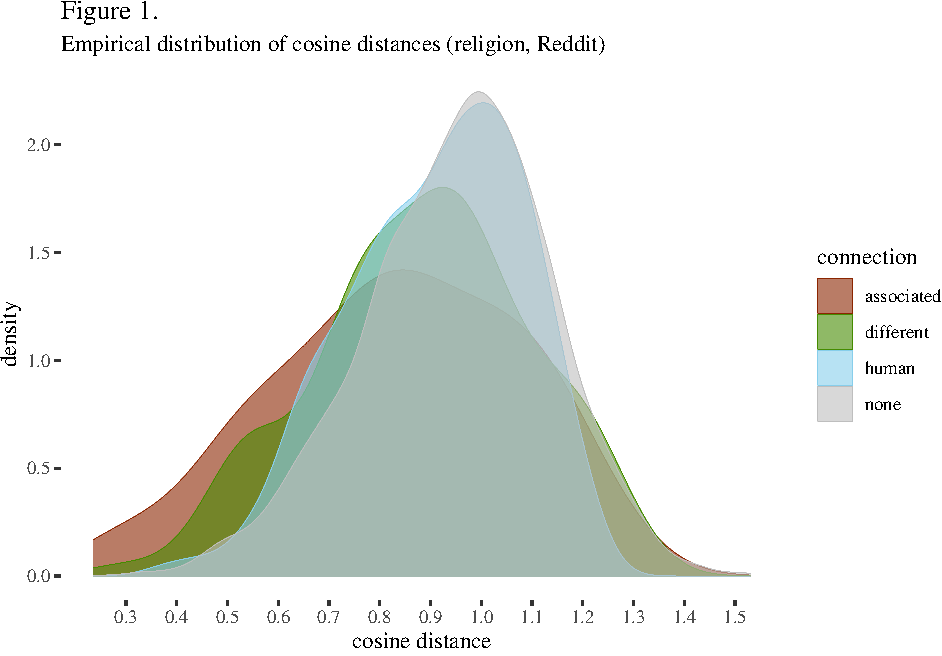
\includegraphics[width=1\linewidth]{_main_files/figure-latex/unnamed-chunk-1-1} \end{center}

\normalsize

The points in the plot above result from the calculation of the inner
product of a chosen vector for a profession word and a vector for a
gender word (she or he). Inner product of two vectors expresses
similarity between words. This assumption originates from the geometry
and properties of a vector space.

\section{Cosine distance in a multi-class bias
detection}\label{cosine-distance-in-a-multi-class-bias-detection}

Manzini et al. (\protect\hyperlink{ref-manzini2019black}{2019}) present
a different approach towards finding similarities between classes of
words. The authors claim that texts available online are full of direct
or indirect human stereotypes. As a result, word embeddings are prone to
learn and maybe amplify those biases and propagate them further into AI
models that are used for various applications. Cosine distance is used
in the article as a measure to first argue for the existence of
multi-class bias and then to show how through bias mitigation techniques
the bias may be decreased.

As the code has been provided by the authors we were able to reconstruct
their results. The main steps in the procedure are as follows. Let us go
through an example that refers to the process of hard debiasing on
religious attributes.

The example refers to the process of hard debiasing on religious
attributes.

\begin{enumerate}
\def\labelenumi{\arabic{enumi}.}
\tightlist
\item
  First we load word embeddings from
  reddit.US.txt.tok.clean.cleanedforw2v.w2v dataset
\end{enumerate}

\begin{itemize}
\tightlist
\item
  The word embeddings have only 50 dimensions
\item
  The number of individual words from the dataset is 44895
\end{itemize}

\begin{enumerate}
\def\labelenumi{\arabic{enumi}.}
\setcounter{enumi}{1}
\tightlist
\item
  The protected group the authors assume should ideally not have high
  cosine similarity to stereotypical words. The word embeddings geometry
  should not place this group close to harmful stereotypes, if it is to
  be bias-free. \newline
\end{enumerate}

For instance, let's look at the religion-related words.

Protected words by religion type:

\textbf{"jew"       : ["judaism", "jew", "synagogue", "torah", "rabbi"]}
\newline
\textbf{"christian" : ["christianity", "christian", "church", "bible", "priest"]}
\newline
\textbf{"muslim"    : ["islam", "muslim", "mosque", "quran", "imam"]}
\newline

Stereotypical words by religion type:

\textbf{"jew"       : ["greedy", "cheap", "hairy", "liberal"]} \newline
\textbf{"christian"       : ["judgemental", "conservative", "familial"]}
\newline
\textbf{"muslim"       : ["violent", "terrorist", "dirty", "uneducated"]}
\newline

We have prepared a table presenting the values of cosine distance for
each protected word with each attribute (stereotype). The part of the
results is shown below.

\footnotesize 

\begin{Shaded}
\begin{Highlighting}[]
\NormalTok{religion <-}\StringTok{ }\KeywordTok{read.csv}\NormalTok{(}\StringTok{"../datasets/religionReddit.csv"}\NormalTok{)[}\OperatorTok{-}\DecValTok{1}\NormalTok{]}
\KeywordTok{colnames}\NormalTok{(religion) <-}\StringTok{ }\KeywordTok{c}\NormalTok{(}\StringTok{"protectedWord"}\NormalTok{,}\StringTok{"wordToCompare"}\NormalTok{,}\StringTok{"wordClass"}\NormalTok{,}
                        \StringTok{"cosineDistance"}\NormalTok{,}\StringTok{"cosineSimilarity"}\NormalTok{,}\StringTok{"connection"}\NormalTok{)}
\NormalTok{religion}\OperatorTok{$}\NormalTok{wordClass <-}\StringTok{ }\KeywordTok{as.factor}\NormalTok{(religion}\OperatorTok{$}\NormalTok{wordClass)}
\KeywordTok{levels}\NormalTok{(religion}\OperatorTok{$}\NormalTok{wordClass) <-}\StringTok{ }\KeywordTok{c}\NormalTok{(}\StringTok{"christian"}\NormalTok{,}\StringTok{"human"}\NormalTok{,}\StringTok{"jewish"}\NormalTok{,}\StringTok{"muslim"}\NormalTok{,}\StringTok{"neutral"}\NormalTok{)}
\KeywordTok{head}\NormalTok{(religion)  }\OperatorTok\StringTok{  }\KeywordTok{kable}\NormalTok{(}\DataTypeTok{format =} \StringTok{"latex"}\NormalTok{,}\DataTypeTok{booktabs=}\NormalTok{T,}
                      \DataTypeTok{linesep =} \StringTok{""}\NormalTok{,  }\DataTypeTok{escape =} \OtherTok{FALSE}\NormalTok{, }
                      \DataTypeTok{caption =} \StringTok{"Head of the religion dataset."}\NormalTok{) }\OperatorTok
\StringTok{                      }\KeywordTok{kable_styling}\NormalTok{(}\DataTypeTok{latex_options=}\KeywordTok{c}\NormalTok{(}\StringTok{"scale_down"}\NormalTok{))}
\end{Highlighting}
\end{Shaded}

\begin{table}

\caption{\label{tab:religionTableHeadEarly}Head of the religion dataset.}
\centering
\resizebox{\linewidth}{!}{
\begin{tabular}[t]{lllrrl}
\toprule
protectedWord & wordToCompare & wordClass & cosineDistance & cosineSimilarity & connection\\
\midrule
judaism & violent & muslim & 0.7141939 & 0.2858061 & different\\
judaism & terrorist & muslim & 0.7461333 & 0.2538667 & different\\
judaism & dirty & muslim & 1.2002599 & -0.2002599 & different\\
judaism & uneducated & muslim & 0.7885469 & 0.2114531 & different\\
judaism & greedy & jewish & 1.0026172 & -0.0026172 & associated\\
judaism & cheap & jewish & 1.2323229 & -0.2323229 & associated\\
\bottomrule
\end{tabular}}
\end{table}

\normalsize

\pagebreak 

In the article there was no analysis of individual distances but the
general look at the data through the usage of mean. The authors
introduced a metric that tries to generalize the presence of bias
through the classification of multi-class bias in groups of words
connected with gender, religion or race. In the process they first take
the mean of cosine distances between a given protected word and
attributes assigned to each stereotype. They do not differentiate
between stereotypes associated with a word and stereotypes associated
with different words (in case of religion, stereotypes characteristic
for Christianity has also cosine distance measured with for instance,
Judaism or Islam). Then, after collecting the list of mean cosine
distances, they average the list to obtain one final value representing
the whole group, in this example religion, for which the final mean of
all mean distances is equal to 0.859.

\begin{enumerate}
\def\labelenumi{\arabic{enumi}.}
\setcounter{enumi}{2}
\tightlist
\item
  In the article the authors also try to remove previously defined
  biases from word embedding.
\end{enumerate}

First they identify the bias subspace using Principal Component Analysis
(PCA) which is a technique for dimensionality reduction. It is applied
here to choose the subspace that contains the greatest amount of
information. There can be many subspaces found in a given group, for
example in terms of religion one can identify at least a few sets that
are to grasp the concept of religion in general: \newline
\textbf{["judaism", "christianity", "islam"]} \newline
\textbf{["jew", "christian", "muslim"]} \newline
\textbf{["synagogue", "church", "mosque"]} \newline

The idea is to find a set that provides enough information to create
from it a vector representing the concept of religion among words. This
strategy is based on the idea that different dimensions of vectors
contain different types of information and in some words in vector
layers (subspaces) the information about religiousness is implicitly
conveyed. In some cases this knowledge is useful but in the case of
harmful stereotypes one does not want to have religion concept in
stereotypical words.

After finding bias subspace, they use it to modify the vector values
individually so that their cosine distances towards certain words are
changed. In the case of stereotypes the aim is to make the cosine
distances larger so that the association between protected word and
harmful stereotype is smaller.

\begin{enumerate}
\def\labelenumi{\arabic{enumi}.}
\setcounter{enumi}{3}
\tightlist
\item
  In the final step there is an evaluation of the results. The cosine
  distances are calculated again but this time using debiased
  vocabulary. After taking the mean of all distances one final value is
  obtained and then it is compared with the average value from the
  beginning. If the cosine distances are on average greater than before
  then it leads the authors to the conclusion that improvement was made.
  As the cosine distance increases it is assumed that the association
  between protected and stereotypical words decreases.
\end{enumerate}

\section{Limitations of the approach}\label{limitations-of-the-approach}

\textbf{1. Selection of attributes}

The attributes are taken from different sources, there is no principled
justification for their choice. From our analysis it will become clear
that the list is rather uneven.

There is no mention of methodology for deciding on the number of
attributes necessary to decide a hypothesis on the given size of
dataset. There are however some ways to estimate how many samples we
need to make sure that the result is significant. Our research will show
that the numbers used are rather insufficient.

\textbf{2. No control while taking the mean of cosines}

The authors use the mean average cosine similarity to check on
multi-class similarity between protected word and harmful stereotypes.
They average the results until they obtain one final value to represent
the mean cosine distance between protected word from a given class and
the attributes of that class. As there is no control of the individual
values of cosine distances, one can observe values that have cosine
distances greater than 1 which would suggest that these compare words do
not have significant similarity. However, as there is a lack of control,
even such words are taken into the account for calculations.

\textbf{3. The lack of uncertainty}

A mean hides this issue and as there are pairs having negative and small
similarities and there are those that have similarity equal to 0.5, the
resulting calculation seems to be in norm. Additionally in such method
the uncertainty is also not included which makes it even more difficult
to give reasonable interpretations of the results. We propose the use of
Bayesian method to obtain some understanding of the influence the
uncertainty has on the interpretation of final results.

\textbf{4. No word class distinction}

In the original paper words from all three religions were checked with
all of the stereotypes which means that there was no distinction on
whether the stereotype is associated with given religion or with the
other. Not all of the stereotypical words should be considered as
harmful for all of the religions. In our analysis we distinguished
between associated stereotypes, not associated (stereotype is valid but
for different religion than currently checked) and none (meaning neutral
words).

\textbf{5. Interpreting the results}

Assuming for a moment that the value of multi-class cosine distance is
correct, one may question the results' interpretation. In Manzini et al.
(\protect\hyperlink{ref-manzini2019black}{2019}) Table 2, there are
summarized the averages of cosine distance per group (gender, race,
religion). I would like to focus now on analyzing the values relating to
religious biases. Here is the fragment of table that refers to that:

\begin{longtable}[]{@{}ll@{}}
\toprule
Religion Debiasing & MAC\tabularnewline
\midrule
\endhead
Biased & 0.859\tabularnewline
Hard Debiased & 0.934\tabularnewline
Soft Debiased (\(\lambda\) = 0.2) & 0.894\tabularnewline
\bottomrule
\end{longtable}

MAC stand for mean average cosine similarity although in reality the
values of cosine distance are stored there. What may attract attention
is the fact that the value of cosine distance in ``Biased'' category is
already quite high even before ``debiasing''. High cosine distance
indicates low cosine similarity between values. One could think that
average cosine similarity equal to approximately 0.141 is not
significant enough to consider it as biased. However the authors aim to
mitigate ``biases'' in vectors with such great distance to make it even
larger. Methodologically there is a question on what basis this small
similarity is still considered as a proof of bias presence.

This is in general the problem of scale and the lack of universal
intervals that could be applied to know whether the cosine similarity is
high enough to considered given words more similar that if we chose them
on random. It seems like similar practice could be beneficial for
metrics aimed at measuring similarity between words.

\textbf{6. The curse of dimensionality}

Curse of dimensionality may take place when there is an increase in
volume of data that results in adding extra dimensions to the Euclidean
space. According to the article
``\url{https://analyticsindiamag.com/curse-of-dimensionality-and-what-beginners-should-do-to-overcome-it/}''
as the number of features increases, it may be harder and harder to
obtain useful information from the data with the usage of available
algorithms. One may notice that more data should contribute to greater
amount of information but more information also means greater risk of
noise and distractions in data. At the same time, many times modern
solutions are adapted to smaller dimensions and their results in higher
ones are not intuitive or may be prone to be mistaken.

Using cosine similarity in high dimensions in word embeddings may also
be prone to the curse of dimensionality. According to this article
``\url{https://www.researchgate.net/publication/327498046_The_Curse_of_Dimensionality_Inside_Out}''
there are reasons to consider this phenomenon when searching for word
similarities in higher dimensions.

In the article an experiment is conducted that aims at showing how the
similarity values and variation change as the number of dimensions
increases. The hypothesis made in the paper states that two things will
happen as the number of dimensions increase, the first one is that
effort required to measure cosine similarity will be greater and the
second one is that the similarity between data will blur out and have
less variation. In details, the authors generate random points with
increasing number of dimensions where each dimension of a data point is
given a value between 0 and 1. Then they pick one vector at random from
each dimension class and calculate cosine similarity between the chosen
vector and the rest of the data. Then they check how the variation of
values changes as the number of dimensions increases. It seems like the
more dimensions there are, the smaller the variance and therefore it is
less obvious how to interpret the resulting cosine similarities. Maybe
the scale should be adjusted to the number of dimensions and variance so
that it still gives us sensible information about data. According to
some researches the cosine similarity in high dimensions is not reliable
enough to trust it as it may be the case that choosing words on random
may result in getting similar values as when picking them consciously.

\begin{figure}
\centering
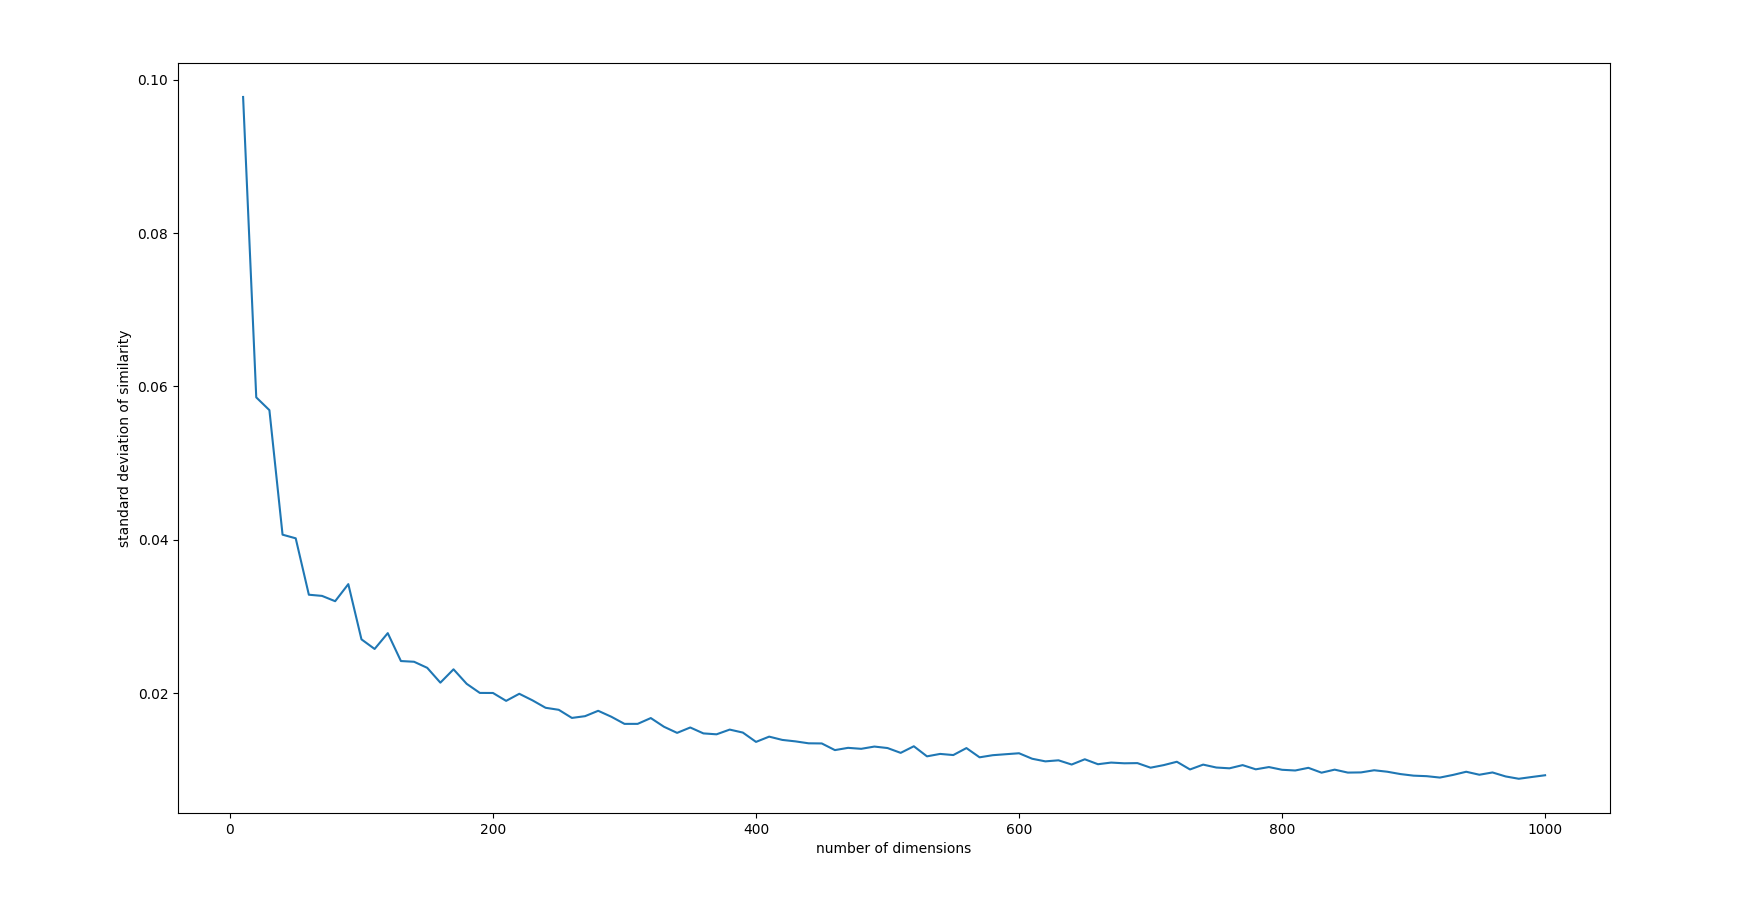
\includegraphics{../images/curseOfDimensionality.png}
\caption{curse of dimensionality, number of dimensions on the x axis,
standard deviation of similarity on the y axis}
\end{figure}

\chapter{Walkthrough with the religion
dataset}\label{walkthrough-with-the-religion-dataset}

\section{Loading and understanding the
dataset}\label{loading-and-understanding-the-dataset}

We start with loading the libraries needed for the analysis.

\footnotesize

\begin{Shaded}
\begin{Highlighting}[]
\KeywordTok{library}\NormalTok{(ggplot2)}
\KeywordTok{library}\NormalTok{(ggthemes)}
\KeywordTok{library}\NormalTok{(rethinking)}
\KeywordTok{library}\NormalTok{(tidyverse)}
\KeywordTok{library}\NormalTok{(ggpubr)}
\KeywordTok{library}\NormalTok{(kableExtra)}
\KeywordTok{library}\NormalTok{(dplyr)}
\KeywordTok{library}\NormalTok{(ggExtra)}
\KeywordTok{library}\NormalTok{(cowplot)}
\end{Highlighting}
\end{Shaded}

\normalsize 

We will use the choice of protected words and stereotypical predicates
used in REF. This is a decent point of departure, not only we want to
compare our method to that of REF, but also because this data format is
fairly general (as contrasted, say, with a set up for binary
stereotypes). Note also that the method we develop here can fairly
easily be run for different stereotypization patterns. Let's start with
explaining the method and its deployment using a dataset obtained for
the religion-related protected words.

Let's load, clean a bit and inspect the head of the religion dataset we
prepared. In order to obtain this dataset, we calculated the cosine
distance between each protected word and each word from both the
bias-related attribute groups, which were used in the original study,
and to neutral and human control attributes which we added as control
groups. For instance, for religion, the bias-related predicates (coming
from the original study in REF) include muslim bias attributes, jew bias
attributes, christian bias attributes (see a list in the APPENDIX).

We decided to add control groups in the form of two classes --- neutral
words and human-related words. Without a proper control group it is
quite hard to compare the resulting cosine distances and decide on their
significance in bias detection. We prepared approximately
300\todo{FIX later} more or less neutral words to double-check the
prima-facie neutral hypothesis that their cosine similarity to the
protected words will oscillate around 0 (that is, the distances will be
around 1). This provides us with a more reliable point of reference.
Moreover, we added human attributes that are associated with people in
general to investigate whether the smaller cosine distance between
protected words and stereotypes can result simply from the fact that the
stereotype predicates are associated with humans. For two control
groups, we have randomly drawn 300 words that do not express any
property usually attributed to humans, and human attributes.
\todo{describe once the words are selected}

\vspace{1mm} \footnotesize

\begin{Shaded}
\begin{Highlighting}[]
\NormalTok{religion <-}\StringTok{ }\KeywordTok{read.csv}\NormalTok{(}\StringTok{"../datasets/religionReddit.csv"}\NormalTok{)[}\OperatorTok{-}\DecValTok{1}\NormalTok{]}
\KeywordTok{colnames}\NormalTok{(religion) <-}\StringTok{ }\KeywordTok{c}\NormalTok{(}\StringTok{"protectedWord"}\NormalTok{,}\StringTok{"wordToCompare"}\NormalTok{,}\StringTok{"wordClass"}\NormalTok{,}
                        \StringTok{"cosineDistance"}\NormalTok{,}\StringTok{"cosineSimilarity"}\NormalTok{,}\StringTok{"connection"}\NormalTok{)}
\CommentTok{#head(religion)}
\CommentTok{#library(plyr)}
\NormalTok{religion}\OperatorTok{$}\NormalTok{wordClass <-}\StringTok{ }\KeywordTok{as.factor}\NormalTok{(religion}\OperatorTok{$}\NormalTok{wordClass)}
\CommentTok{#levels(religion$wordClass)}
\CommentTok{#religion$wordClass <- mapvalues(religion$wordClass, }
\CommentTok{#                          from = levels(religion$wordClass),}
\CommentTok{#                          to = c("christian","human","jewish","muslim","neutral"))}
\KeywordTok{levels}\NormalTok{(religion}\OperatorTok{$}\NormalTok{wordClass) <-}\StringTok{ }\KeywordTok{c}\NormalTok{(}\StringTok{"christian"}\NormalTok{,}\StringTok{"human"}\NormalTok{,}\StringTok{"jewish"}\NormalTok{,}\StringTok{"muslim"}\NormalTok{,}\StringTok{"neutral"}\NormalTok{)}
\KeywordTok{head}\NormalTok{(religion)  }\OperatorTok\StringTok{  }\KeywordTok{kable}\NormalTok{(}\DataTypeTok{format =} \StringTok{"latex"}\NormalTok{,}\DataTypeTok{booktabs=}\NormalTok{T,}
                      \DataTypeTok{linesep =} \StringTok{""}\NormalTok{,  }\DataTypeTok{escape =} \OtherTok{FALSE}\NormalTok{, }
                      \DataTypeTok{caption =} \StringTok{"Head of the religion dataset."}\NormalTok{) }\OperatorTok\StringTok{      }\KeywordTok{kable_styling}\NormalTok{(}\DataTypeTok{latex_options=}\KeywordTok{c}\NormalTok{(}\StringTok{"scale_down"}\NormalTok{))}
\end{Highlighting}
\end{Shaded}

\begin{table}

\caption{\label{tab:religionTableHead}Head of the religion dataset.}
\centering
\resizebox{\linewidth}{!}{
\begin{tabular}[t]{lllrrl}
\toprule
protectedWord & wordToCompare & wordClass & cosineDistance & cosineSimilarity & connection\\
\midrule
judaism & violent & muslim & 0.7141939 & 0.2858061 & different\\
judaism & terrorist & muslim & 0.7461333 & 0.2538667 & different\\
judaism & dirty & muslim & 1.2002599 & -0.2002599 & different\\
judaism & uneducated & muslim & 0.7885469 & 0.2114531 & different\\
judaism & greedy & jewish & 1.0026172 & -0.0026172 & associated\\
judaism & cheap & jewish & 1.2323229 & -0.2323229 & associated\\
\bottomrule
\end{tabular}}
\end{table}

\normalsize

The \texttt{protectedWord} column contains words from a protected class
that (in a perfect world according to the assumptions of the orignal
study) should not be associated with harmful stereotypes.
\texttt{wordToCompare} contains attributes, including stereotypes and
control group words. For each row we compute the cosine distances
between a given protected word and a given attribute word.
\texttt{wordClass} tells us which class an attribute is supposed to be
stereotypically associated with, that is, whether the word from
\texttt{wordToCompare} is associated stereotypically with jews,
christians or muslims, or whether it belongs to a control group.
\texttt{cosineDistance} is simply a calculation of the cosine distance
between protected word and atrribute. \texttt{cosineSimilarity} contains
the result of substracting cosine distance from 1. \texttt{connection}
contains information about the relation type between a protected word
and an attribute. If the attribute is e.g.~a harmful jewish stereotype
and the protected word is also from the judaism group, the connection
has value \texttt{associated}. If the attribute is still stereotypically
jewish, but the protected word comes from another religion, the
connection is labelled as \texttt{different}. If the attribute belongs
to a neutral group then the connection is labelled as \texttt{none} and
if an attribute belongs to the \texttt{human} class, then the connection
is labelled as \texttt{human}.

\section{First look at the empirical
distributions}\label{first-look-at-the-empirical-distributions}

First let's take a look at the empirical distribution of distances by
the connection type, initially ignoring the human control class for now.

\vspace{1mm} \footnotesize

\begin{center}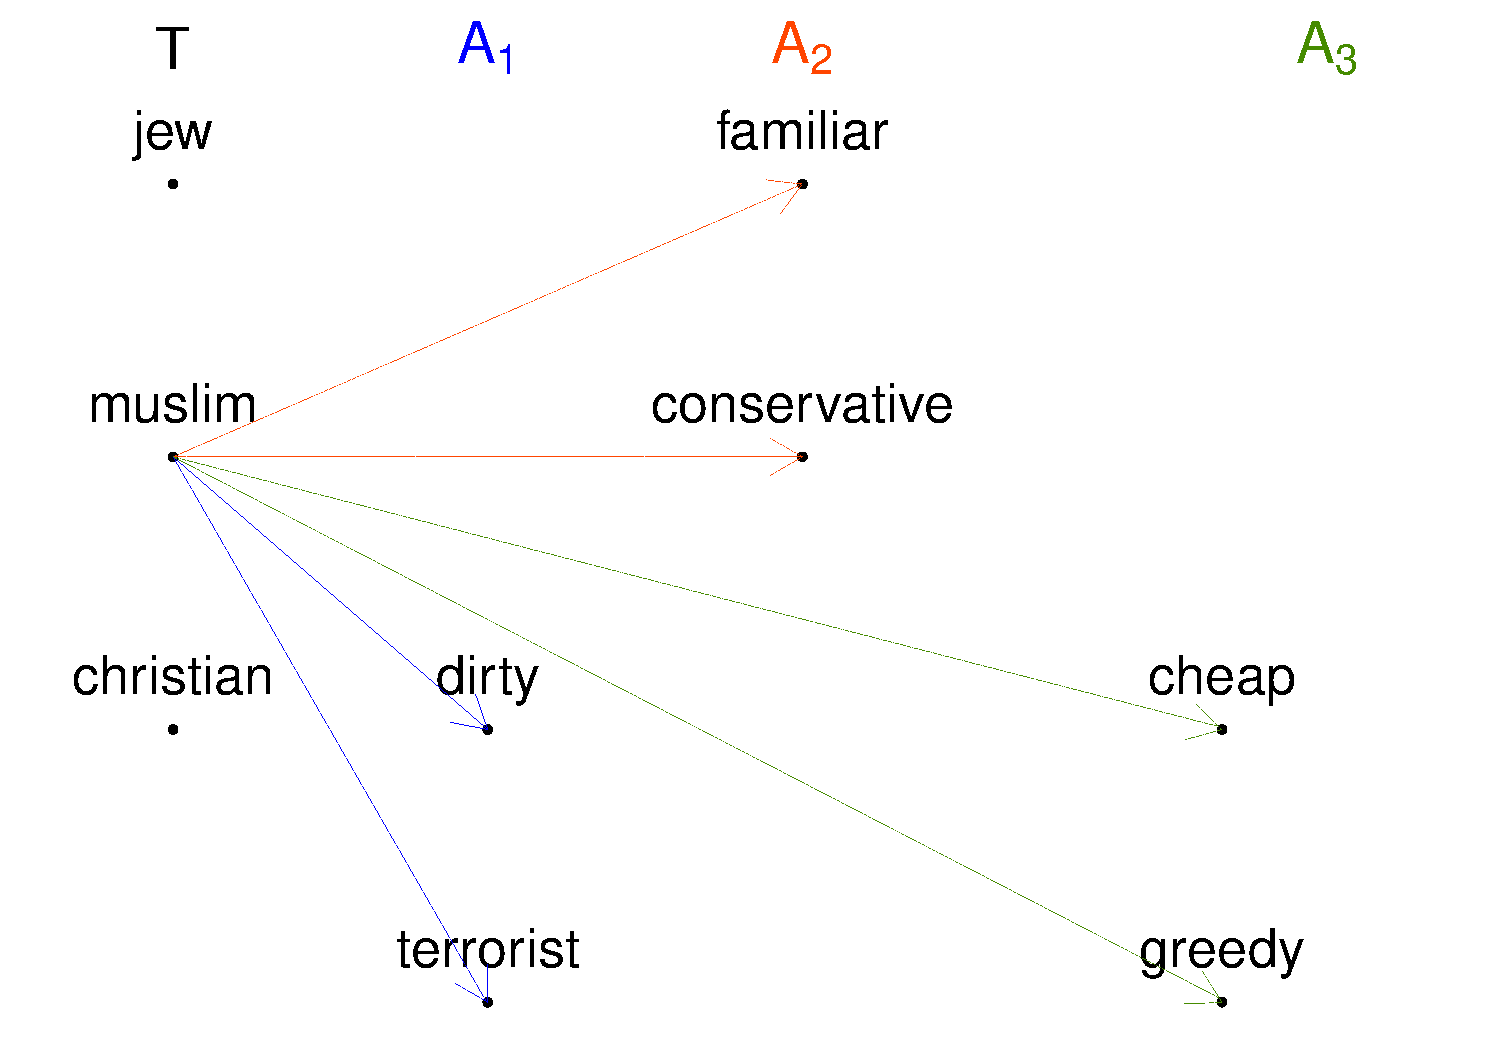
\includegraphics[width=1\linewidth]{_main_files/figure-latex/unnamed-chunk-3-1} \end{center}

\normalsize

The first impression is that while there is a shift for associated words
towards smaller cosine distances as compared to the neutral words,
slightly surprisingly a slightly weaker shift in the same direction is
visible for attributes associated with different stereotypes. Moreover,
the empirical distributions overlap to alarge extent and the means
grouped by connection type do not seem too far from each other. In fact,
as there is a lot of variety in the consine distances (as we will soon
see), abd we need to gauge the uncertaintly involved, and to look more
carefully at individual protected words to get a better idea of how the
cosine distance distribution changes for different attribute groups and
different protected classes. Now, let's add the human attributes to the
picture:

\vspace{1mm} \footnotesize

\begin{center}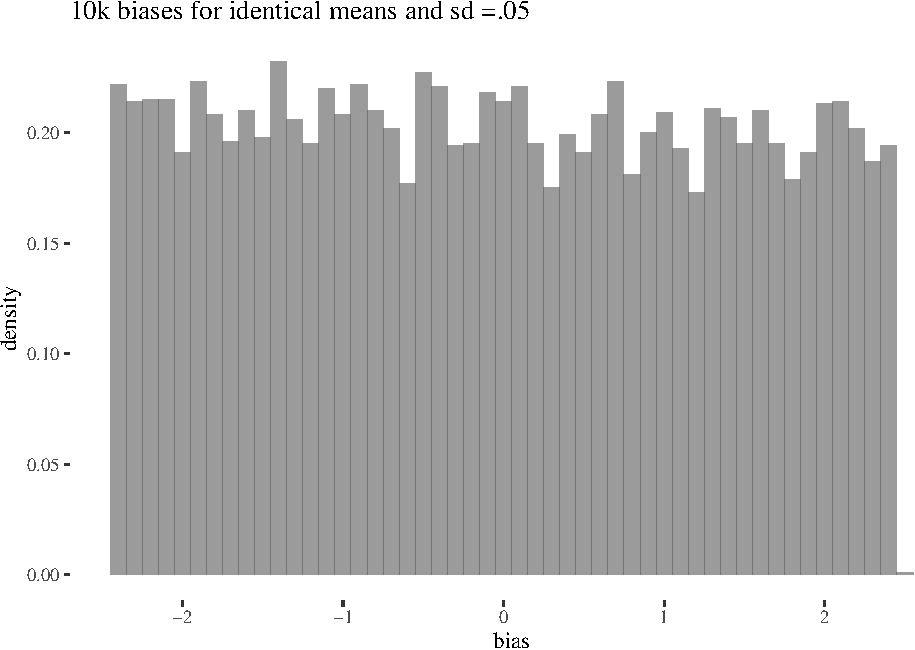
\includegraphics[width=1\linewidth]{_main_files/figure-latex/unnamed-chunk-4-1} \end{center}

\normalsize

\noindent Notice that the distribution for \texttt{human} (even though
we did our best not to include in it any stereotype-related atributes)
is left-skewed, with much overlap with \texttt{associated} and
\texttt{different}, which illustrates the need to take being associated
with humans as an important predictor.

Our focus lies in \texttt{connection} as a predictor. Morever, later on
we'll be interested in looking at the protected words separately, and at
protected words split by connection. For technical reasons it is useful
to represent these factors as integer vectors.

\vspace{1mm} \footnotesize

\begin{Shaded}
\begin{Highlighting}[]
\NormalTok{religion}\OperatorTok{$}\NormalTok{con <-}\StringTok{ }\KeywordTok{as.integer}\NormalTok{(religion}\OperatorTok{$}\NormalTok{connection)}
\NormalTok{religion}\OperatorTok{$}\NormalTok{pw <-}\StringTok{ }\KeywordTok{as.integer}\NormalTok{(religion}\OperatorTok{$}\NormalTok{protectedWord)}
\NormalTok{religion}\OperatorTok{$}\NormalTok{pwFactor <-}\StringTok{ }\KeywordTok{factor}\NormalTok{(}\KeywordTok{paste0}\NormalTok{(religion}\OperatorTok{$}\NormalTok{protectedWord, religion}\OperatorTok{$}\NormalTok{connection))}
\NormalTok{religion}\OperatorTok{$}\NormalTok{pwIndex <-}\StringTok{ }\KeywordTok{as.integer}\NormalTok{(religion}\OperatorTok{$}\NormalTok{pwFactor)}
\end{Highlighting}
\end{Shaded}

\normalsize

A short script, \texttt{cleanDataset} to make this faster, so
equivalently:

\vspace{1mm} \footnotesize

\begin{Shaded}
\begin{Highlighting}[]
\KeywordTok{source}\NormalTok{(}\StringTok{"../functions/cleanDataset.R"}\NormalTok{)}
\NormalTok{religion <-}\StringTok{ }\KeywordTok{read.csv}\NormalTok{(}\StringTok{"../datasets/religionReddit.csv"}\NormalTok{)[}\OperatorTok{-}\DecValTok{1}\NormalTok{]}
\NormalTok{religion <-}\StringTok{ }\KeywordTok{cleanDataset}\NormalTok{(religion,}\KeywordTok{c}\NormalTok{(}\StringTok{"christian"}\NormalTok{,}\StringTok{"human"}\NormalTok{,}\StringTok{"jewish"}\NormalTok{,}\StringTok{"muslim"}\NormalTok{,}\StringTok{"neutral"}\NormalTok{))}
\end{Highlighting}
\end{Shaded}

\normalsize

\section{Looking at the islam-related
words}\label{looking-at-the-islam-related-words}

For now, let's focus on five protected words related to islam (``imam'',
``islam'', ``mosque'', ``muslim'', and ``quran''). The word list
associates with islam four stereotypical attributes (``violent'',
``terrorist'', ``uneducated'' and ``dirty''). First, we select and plot
the empirical distributions for these protected words.

\vspace{1mm} \footnotesize

\begin{Shaded}
\begin{Highlighting}[]
\KeywordTok{library}\NormalTok{(tidyverse)}
\NormalTok{muslimWords <-}\StringTok{ }\KeywordTok{c}\NormalTok{(}\StringTok{"imam"}\NormalTok{,}\StringTok{"islam"}\NormalTok{,}\StringTok{"mosque"}\NormalTok{,}\StringTok{"muslim"}\NormalTok{,}\StringTok{"quran"}\NormalTok{)}
\NormalTok{muslim <-}\StringTok{ }\NormalTok{religion }\OperatorTok\StringTok{ }\KeywordTok{filter}\NormalTok{(protectedWord }\OperatorTok\StringTok{ }\NormalTok{muslimWords)}
\KeywordTok{ggplot}\NormalTok{(muslim, }\KeywordTok{aes}\NormalTok{(}\DataTypeTok{x =}\NormalTok{  cosineDistance, }\DataTypeTok{fill =}\NormalTok{ connection, }\DataTypeTok{color =}\NormalTok{ connection))}\OperatorTok{+}
\StringTok{  }\KeywordTok{geom_density}\NormalTok{(}\DataTypeTok{alpha=}\FloatTok{0.6}\NormalTok{,}\DataTypeTok{size =} \FloatTok{.2}\NormalTok{)}\OperatorTok{+}\StringTok{ }
\StringTok{  }\KeywordTok{scale_fill_manual}\NormalTok{(}\DataTypeTok{values =} \KeywordTok{c}\NormalTok{(}\StringTok{"orangered4"}\NormalTok{,}\StringTok{"chartreuse4"}\NormalTok{, }\StringTok{"skyblue"}\NormalTok{, }\StringTok{"gray"}\NormalTok{))}\OperatorTok{+}
\StringTok{  }\KeywordTok{scale_x_continuous}\NormalTok{(}\DataTypeTok{breaks =} \KeywordTok{seq}\NormalTok{(}\FloatTok{0.3}\NormalTok{,}\FloatTok{1.5}\NormalTok{, }\DataTypeTok{by =} \FloatTok{0.1}\NormalTok{))}\OperatorTok{+}\KeywordTok{xlab}\NormalTok{(}\StringTok{"cosine distance"}\NormalTok{)}\OperatorTok{+}
\StringTok{  }\KeywordTok{scale_color_manual}\NormalTok{(}\DataTypeTok{values =} \KeywordTok{c}\NormalTok{(}\StringTok{"orangered4"}\NormalTok{,}\StringTok{"chartreuse4"}\NormalTok{,}\StringTok{"skyblue"}\NormalTok{,}\StringTok{"gray"}\NormalTok{))}\OperatorTok{+}
\StringTok{  }\KeywordTok{theme_tufte}\NormalTok{()}\OperatorTok{+}\KeywordTok{ggtitle}\NormalTok{(}\StringTok{"Empirical distribution of distances (muslim)"}\NormalTok{)}
\end{Highlighting}
\end{Shaded}

\begin{center}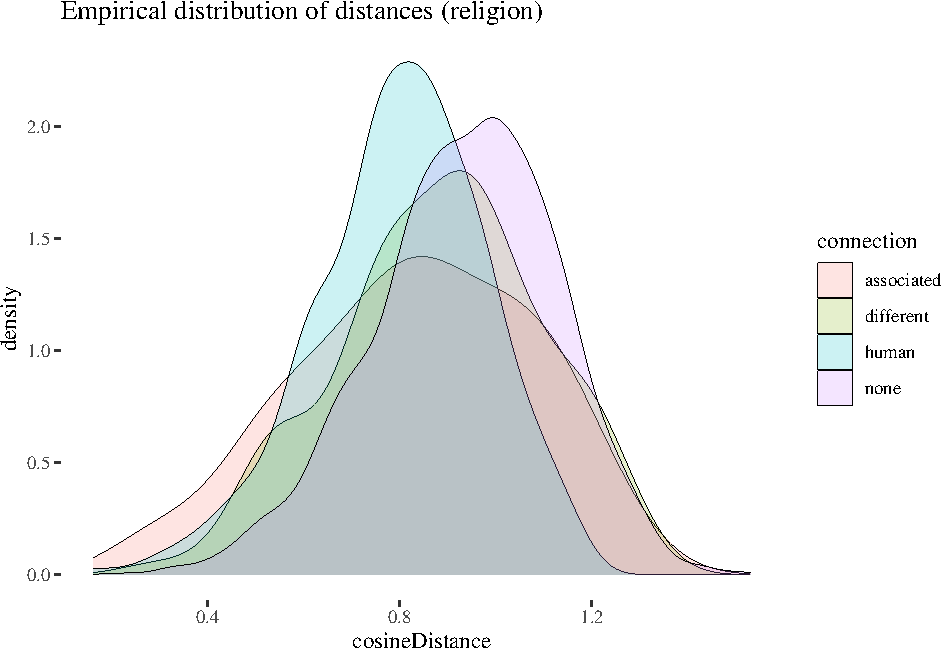
\includegraphics[width=1\linewidth]{_main_files/figure-latex/unnamed-chunk-7-1} \end{center}

\normalsize

\noindent Once we focus on words related to islam, the associated bias
seems to be stronger than in the whole dataset. This is a step towards
illustrating that the distribution of bias is uneven.

Now, say we want to look at a single protected word. Since the dataset
also contains comparison multiple control neutral and human attributes,
we randomly select only 5 from \texttt{none} and 5 from \texttt{human}
control groups of those for the visualisation purposes.

\vspace{1mm} \footnotesize

\begin{Shaded}
\begin{Highlighting}[]
\KeywordTok{library}\NormalTok{(tidyverse)}
\NormalTok{muslimClass <-}\StringTok{ }\NormalTok{muslim }\OperatorTok\StringTok{ }\KeywordTok{filter}\NormalTok{(protectedWord }\OperatorTok{==}\StringTok{ "muslim"}\NormalTok{)}
\NormalTok{neutralSample <-}\StringTok{ }\KeywordTok{sample_n}\NormalTok{(}\KeywordTok{filter}\NormalTok{(muslimClass,connection }\OperatorTok{==}\StringTok{ "none"}\NormalTok{), }\DecValTok{5}\NormalTok{)}
\NormalTok{humanSample <-}\StringTok{ }\KeywordTok{sample_n}\NormalTok{(}\KeywordTok{filter}\NormalTok{(muslimClass,connection }\OperatorTok{==}\StringTok{ "human"}\NormalTok{), }\DecValTok{5}\NormalTok{)}
\NormalTok{muslimVis <-}\StringTok{ }\NormalTok{muslimClass }\OperatorTok\StringTok{ }\KeywordTok{filter}\NormalTok{(connection }\OperatorTok{!=}\StringTok{ "none"} \OperatorTok{&}\StringTok{ }\NormalTok{connection }\OperatorTok{!=}\StringTok{"human"}\NormalTok{)}
\NormalTok{muslimVis <-}\StringTok{ }\KeywordTok{rbind}\NormalTok{(muslimVis,neutralSample,humanSample)}

\CommentTok{#we plug in our visualisation script}
\KeywordTok{source}\NormalTok{(}\StringTok{"../functions/visualisationTools.R"}\NormalTok{)}
\CommentTok{#two arguments: dataset and protected word}
\KeywordTok{visualiseProtected}\NormalTok{(muslimVis,}\StringTok{"muslim"}\NormalTok{)}
\end{Highlighting}
\end{Shaded}

\begin{center}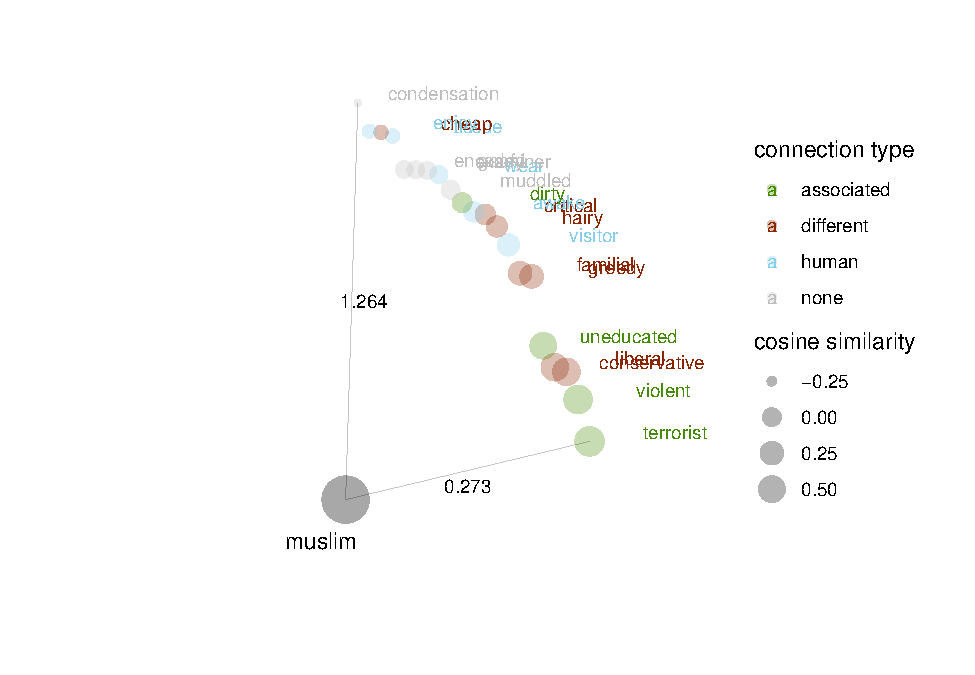
\includegraphics[width=1\linewidth]{_main_files/figure-latex/tableMuslimActive-1} \end{center}

\normalsize

Note that the distance between the grey point and the other points is
proportional to cosine distance, the non-grey point size is proportional
to cosine similarity to the protected word, and color groups by the
connection type. So for \texttt{muslim} it seems that the stereotypes
coming from the word list are fairly well visible. To give you some
taste of how uneven the dataset is, compare this to what happens with
\texttt{priest}.

\vspace{1mm} \footnotesize

\begin{Shaded}
\begin{Highlighting}[]
\KeywordTok{library}\NormalTok{(tidyverse)}
\NormalTok{priestClass <-}\StringTok{ }\NormalTok{religion }\OperatorTok\StringTok{ }\KeywordTok{filter}\NormalTok{(protectedWord }\OperatorTok{==}\StringTok{ "priest"}\NormalTok{)}
\NormalTok{neutralSample <-}\StringTok{ }\KeywordTok{sample_n}\NormalTok{(}\KeywordTok{filter}\NormalTok{(priestClass,connection }\OperatorTok{==}\StringTok{ "none"}\NormalTok{), }\DecValTok{5}\NormalTok{)}
\NormalTok{humanSample <-}\StringTok{ }\KeywordTok{sample_n}\NormalTok{(}\KeywordTok{filter}\NormalTok{(priestClass,connection }\OperatorTok{==}\StringTok{ "human"}\NormalTok{), }\DecValTok{5}\NormalTok{)}
\NormalTok{priestVis <-}\StringTok{ }\NormalTok{priestClass }\OperatorTok\StringTok{ }\KeywordTok{filter}\NormalTok{(connection }\OperatorTok{!=}\StringTok{ "none"} \OperatorTok{&}\StringTok{ }\NormalTok{connection }\OperatorTok{!=}\StringTok{"human"}\NormalTok{)}
\NormalTok{priestVis <-}\StringTok{ }\KeywordTok{rbind}\NormalTok{(priestVis,neutralSample,humanSample)}

\CommentTok{#we plug in our visualisation script}
\KeywordTok{source}\NormalTok{(}\StringTok{"../functions/visualisationTools.R"}\NormalTok{)}
\CommentTok{#two arguments: dataset and protected word}
\KeywordTok{visualiseProtected}\NormalTok{(priestVis,}\StringTok{"priest"}\NormalTok{)}
\end{Highlighting}
\end{Shaded}

\begin{center}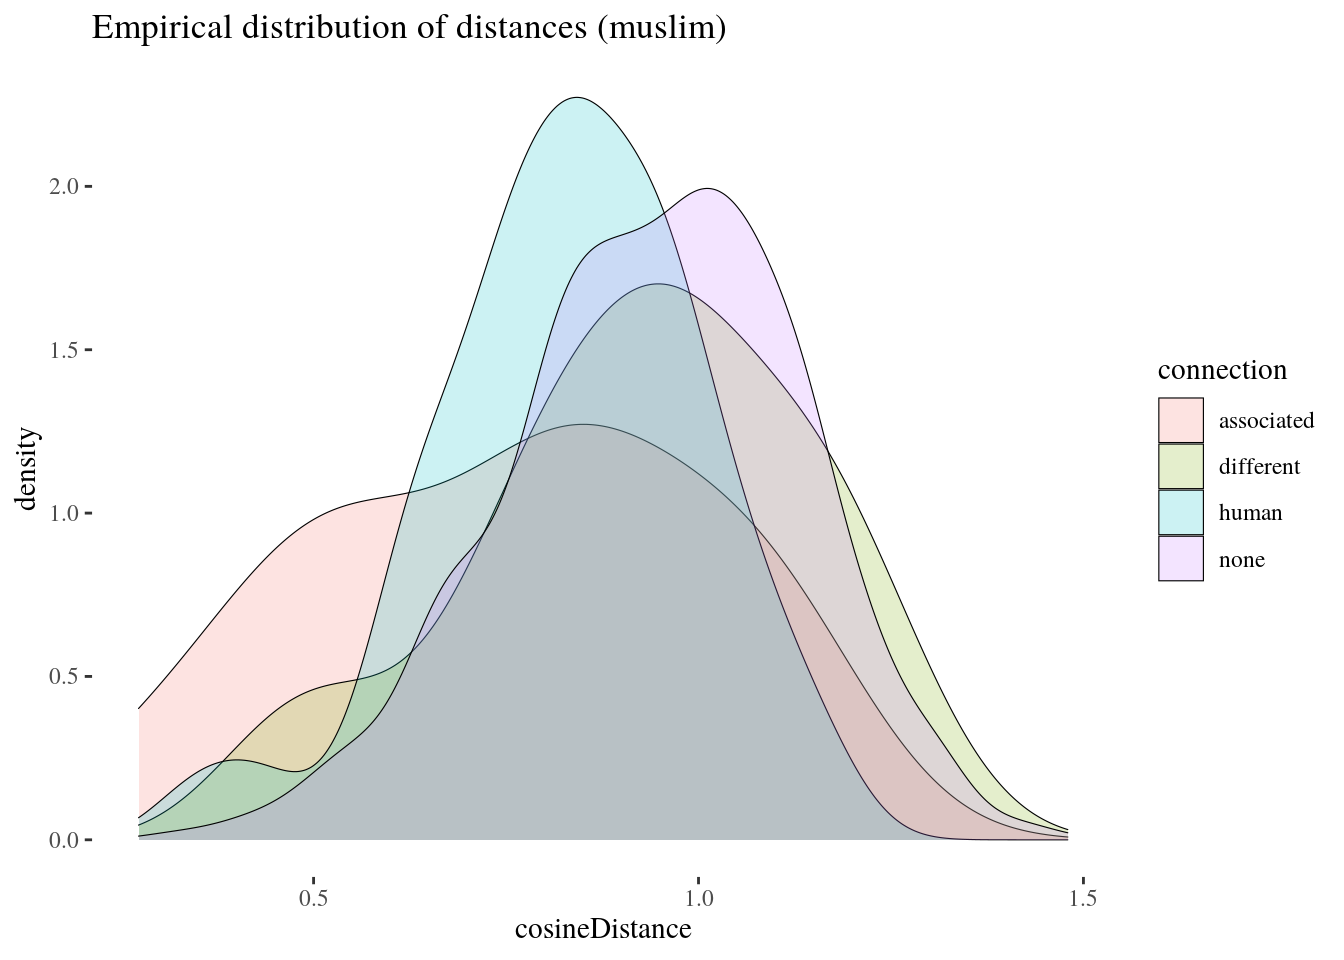
\includegraphics[width=1\linewidth]{_main_files/figure-latex/unnamed-chunk-8-1} \end{center}

\normalsize

\noindent Here you can see that some human attributes are closer than
stereotype attributes, and that there is no clear reason to claim that
\texttt{associated} attributes are closer than \texttt{different} or
\texttt{human} attributes. This, again, illustrates the need of
case-by-case analysis with control groups.

The general idea now is that the word lists provided in different pieces
of research are just samples of attributes associates with various
stereotypes and should be treated as such: the uncertaintly involved and
the sample sizes should have clear impact on our estimates.

\section{Bayesian model structure and
assumptions}\label{bayesian-model-structure-and-assumptions}

We will now think of cosine distance as the output variable, and will
build a few bayesian models to compare. First, we just build a baseline
model which estimates cosine distance to the attributes separately for
each protected word. The underlying idea is that different protected
words migh in general have different relations to all the attributes and
this relations should be our point of departure.

Here is the intution behind the mathematical Bayesian model involved.
Our outcome variable is \texttt{cosine\ difference}, which we take to me
normally distributed around the predicted mean for a given protected
word (that is, we assume the residuals are normally distributed). The
simplest model specification is:

\begin{align}
cosineDistance_i  & \sim dnorm(\mu_i, \sigma) \\
\mu_i & = m_{pw} \\
m_{pw} & ~ dnorm(1,.5) \\
\sigma &\sim  dcauchy(0,1)
\end{align}

That is, we assume the estimated means might be different for diferent
protected words and our prior for the mean and the overal standard
deviation are normal with mean 1 and sd=.5 and half-cauchy with
parameters \texttt{0,1}. Further on we'll also estimate additional
impact the connection type may have. For this impact we take a slightly
skeptical prior centered around 0 distributed normally with sd = 1.
These are fairly weak and slightly skeptical regularizing priors, which
can be illustrated as follows:

\vspace{2mm}

\begin{center}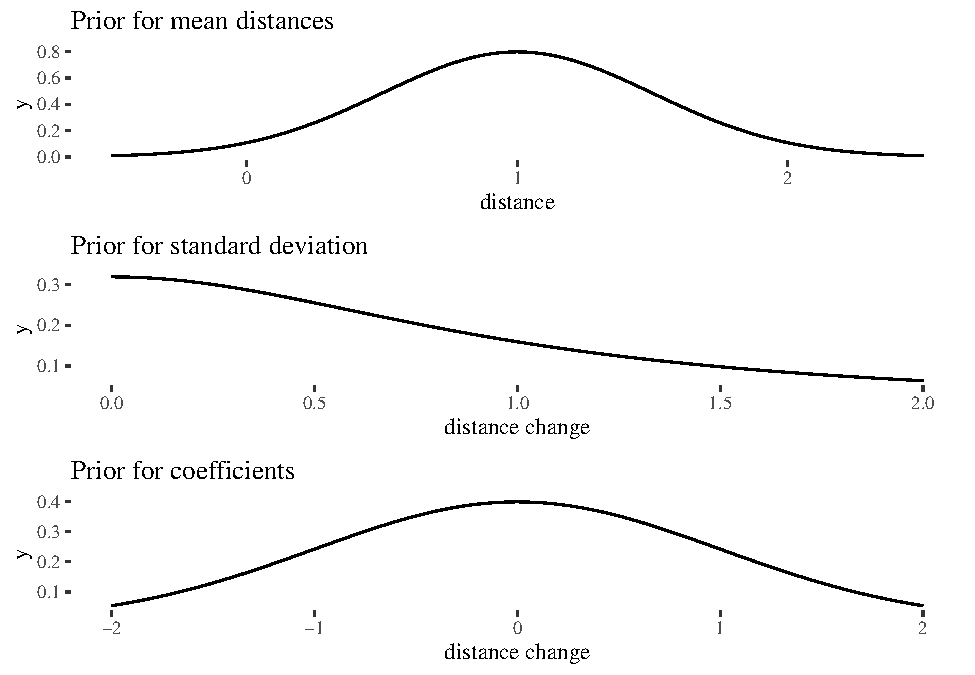
\includegraphics[width=1\linewidth]{_main_files/figure-latex/priorsVis-1} \end{center}

\section{Choosing predictors}\label{choosing-predictors}

Now we can define and compile the baseline model. Its parameters will
have a posterior distribution obtained using either Hamiltionian Monte
Carlo methods (STAN) available through the \texttt{rethinking} package.

\vspace{1mm} \footnotesize

\begin{Shaded}
\begin{Highlighting}[]
\KeywordTok{library}\NormalTok{(rethinking)}
\KeywordTok{options}\NormalTok{(}\DataTypeTok{buildtools.check =} \ControlFlowTok{function}\NormalTok{(action) }\OtherTok{TRUE}\NormalTok{ )}
\NormalTok{religionBaseline <-}\StringTok{ }\KeywordTok{ulam}\NormalTok{(}
  \KeywordTok{alist}\NormalTok{(}
\NormalTok{    cosineDistance }\OperatorTok{~}\StringTok{ }\KeywordTok{dnorm}\NormalTok{(mu,sigma),}
\NormalTok{    mu <-}\StringTok{ }\NormalTok{m[pw],}
\NormalTok{    m[pw] }\OperatorTok{~}\StringTok{ }\KeywordTok{dnorm}\NormalTok{(}\DecValTok{1}\NormalTok{,.}\DecValTok{5}\NormalTok{),}
\NormalTok{    sigma }\OperatorTok{~}\StringTok{ }\KeywordTok{dcauchy}\NormalTok{(}\DecValTok{0}\NormalTok{,}\DecValTok{1}\NormalTok{)}
\NormalTok{  ),}
  \DataTypeTok{data =}\NormalTok{ religion,}
  \DataTypeTok{chains=}\DecValTok{2}\NormalTok{ , }\DataTypeTok{iter=}\DecValTok{4000}\NormalTok{ , }\DataTypeTok{warmup=}\DecValTok{1000}\NormalTok{,}
  \DataTypeTok{start=} \KeywordTok{list}\NormalTok{(}\DataTypeTok{mu =} \DecValTok{1}\NormalTok{, }\DataTypeTok{co =} \DecValTok{0}\NormalTok{, }\DataTypeTok{sigma=} \FloatTok{.3}\NormalTok{),}
  \DataTypeTok{log_lik =} \OtherTok{TRUE}\NormalTok{, }\DataTypeTok{cores=}\DecValTok{4}
\NormalTok{)}
\CommentTok{#saving}
\CommentTok{#saveRDS(religionBaseline, }
\CommentTok{#file = "cosineAnalysis/models/religionBaseline.rds")}
\end{Highlighting}
\end{Shaded}

The only reason we need it is the evaluation of connection as a
predictor. Does including it in o the model improve the situation? To
investigate this, let's now build a model according to the following
specification:

\begin{align}
cosineDistance_i  & \sim dnorm(\mu_i, \sigma) \\
\mu_i & = m_{pw} + co_{con}\\
m_{pw} & ~ dnorm(1,.5) \\
co_{con} & ~ dnorm(0,1) \\
\sigma &\sim  dcauchy(0,1)
\end{align}

\noindent The idea now is that each connection type comes with its own
coefficient \(co\) that has impact on mean distances for protected words
taken separately.

\vspace{1mm} \footnotesize

\begin{Shaded}
\begin{Highlighting}[]
\KeywordTok{library}\NormalTok{(rethinking)}
\KeywordTok{options}\NormalTok{(}\DataTypeTok{buildtools.check =} \ControlFlowTok{function}\NormalTok{(action) }\OtherTok{TRUE}\NormalTok{ )}
\NormalTok{religionCoefs <-}\StringTok{ }\KeywordTok{ulam}\NormalTok{(}
  \KeywordTok{alist}\NormalTok{(}
\NormalTok{    cosineDistance }\OperatorTok{~}\StringTok{ }\KeywordTok{dnorm}\NormalTok{(mu,sigma),}
\NormalTok{    mu <-}\StringTok{ }\NormalTok{m[pw] }\OperatorTok{+}\StringTok{ }\NormalTok{co[con],}
\NormalTok{    m[pw] }\OperatorTok{~}\StringTok{ }\KeywordTok{dnorm}\NormalTok{(}\DecValTok{1}\NormalTok{,.}\DecValTok{5}\NormalTok{),}
\NormalTok{    co[con] }\OperatorTok{~}\KeywordTok{dnorm}\NormalTok{(}\DecValTok{0}\NormalTok{,.}\DecValTok{5}\NormalTok{),}
\NormalTok{    sigma }\OperatorTok{~}\StringTok{ }\KeywordTok{dcauchy}\NormalTok{(}\DecValTok{0}\NormalTok{,}\DecValTok{1}\NormalTok{)}
\NormalTok{  ),}
  \DataTypeTok{data =}\NormalTok{ religion,}
  \DataTypeTok{chains=}\DecValTok{2}\NormalTok{ , }\DataTypeTok{iter=}\DecValTok{8000}\NormalTok{ , }\DataTypeTok{warmup=}\DecValTok{1000}\NormalTok{, }
  \DataTypeTok{log_lik =} \OtherTok{TRUE}
\NormalTok{)}
\end{Highlighting}
\end{Shaded}

\normalsize

\noindent First, let's see if this model is really better in terms of
the Widely Acceptable Information Criterion (WAIC):

\vspace{1mm} \footnotesize

\begin{verbatim}
##                   WAIC SE dWAIC dSE pWAIC weight
## religionCoefs    -2328 93     0  NA    20      1
## religionBaseline -2283 95    45  17    16      0
\end{verbatim}

\normalsize

Clearly, it should be given weight 1 as compared to the baseline model.
So far, we've learned that the connection type actually has predictive
value. Let's take a look at the coefficient estimates:

\vspace{1mm} \footnotesize

\begin{verbatim}
##              mean        sd       5.5%      94.5%    n_eff    Rhat4
## co[1] -0.14956420 0.1151675 -0.3261650 0.03741930 294.2033 1.001449
## co[2] -0.09880543 0.1145024 -0.2736985 0.08813271 291.5044 1.001564
## co[3] -0.07282752 0.1133894 -0.2447778 0.11158986 287.7820 1.001627
## co[4] -0.03103179 0.1131420 -0.2034442 0.15268770 286.8283 1.001606
\end{verbatim}

\normalsize

\section{Dataset-level coefficients}\label{dataset-level-coefficients}

\noindent Let's plot them together with their highest posterior density
invervals, for the three topic groups.

\begin{center}
\begin{figure}[!htb]\centering
   \begin{minipage}{0.55\textwidth}
  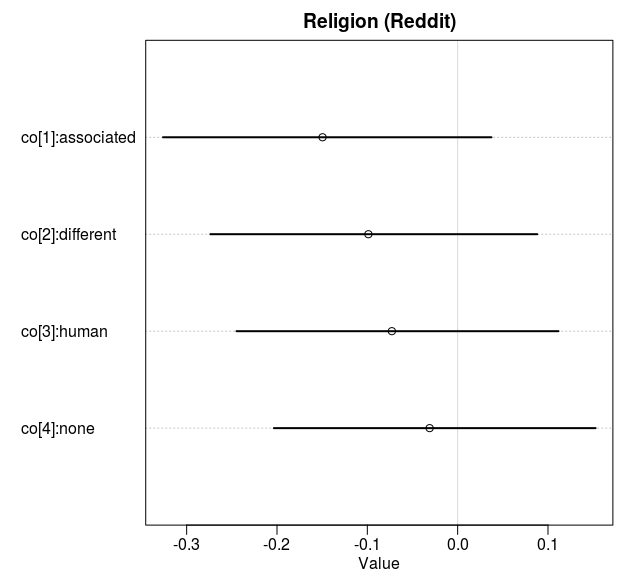
\includegraphics[width=7cm]{../images/religionCoeffs.jpeg}
   \end{minipage}
   \begin {minipage}{0.43\textwidth}
    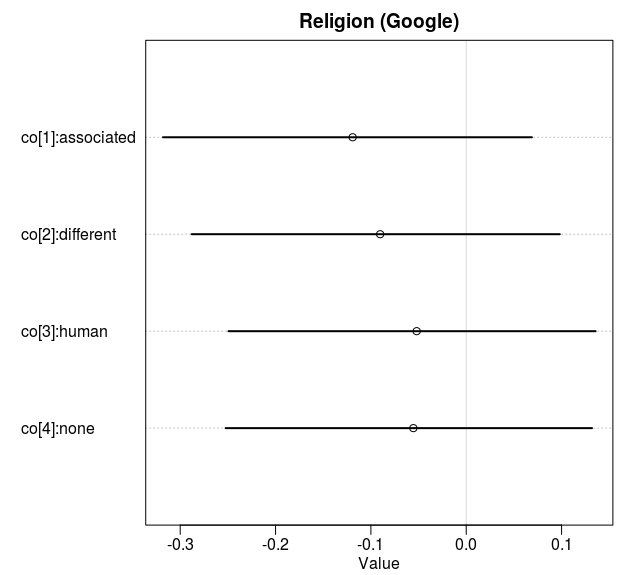
\includegraphics[width=7cm]{../images/religionGoogleCoeffs.jpeg}
   \end{minipage}
   
   
  \begin{minipage}{0.55\textwidth}
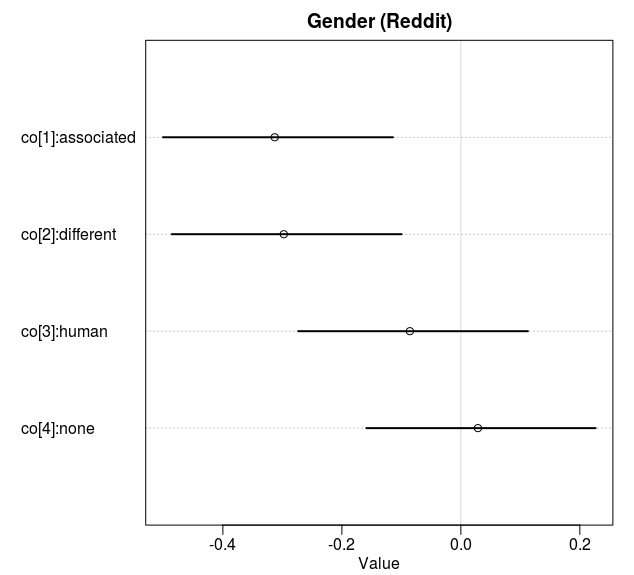
\includegraphics[width=7cm]{../images/genderCoeffs.jpeg}
\end{minipage}
   \begin {minipage}{0.43\textwidth}
    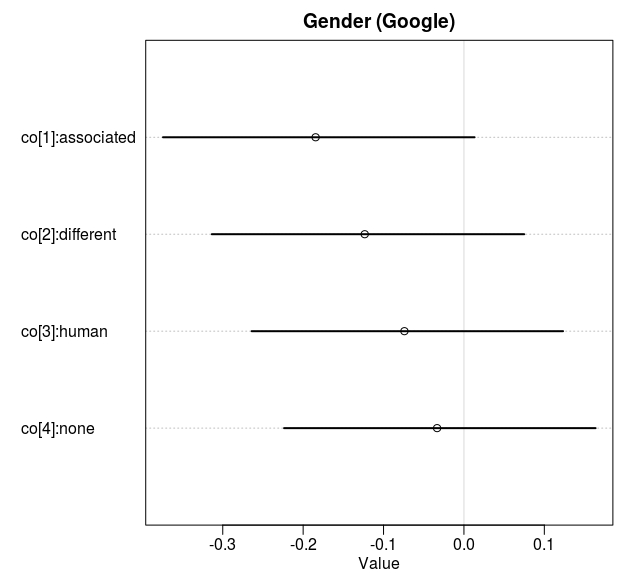
\includegraphics[width=7cm]{../images/genderGoogleCoeffs.jpeg}
   \end{minipage}
   
   
   
   
  \begin{minipage}{0.55\textwidth}
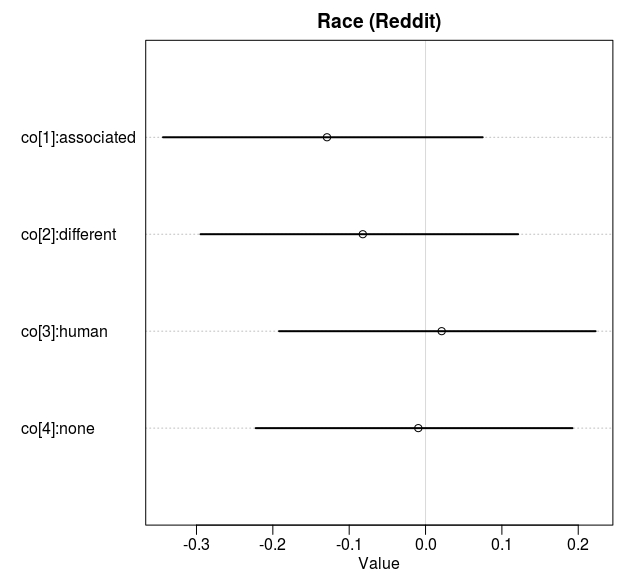
\includegraphics[width=7cm]{../images/raceCoeffs.jpeg}
\end{minipage}
   \begin {minipage}{0.43\textwidth}
    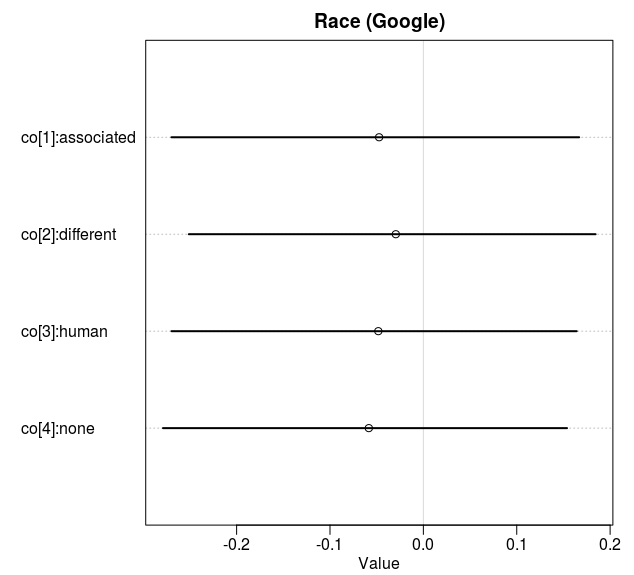
\includegraphics[width=7cm]{../images/raceGoogleCoeffs.jpeg}
   \end{minipage}
\end{figure}


\end{center}

\noindent What should strike us is that while the mean estimates of the
coefficients indeed do differ a bit, usually the highest posterior
density invervals all include zero, and so we do not have strong reasons
to say that, say, as far as the whole religion dataset is involved,
being associated indeed is connected with lower cosine distance. A
second striking observation is that the estimated impact for associated
stereotypes is quite often not too different from the estimated impact
of attributes associated with different stereotypes, and both are
sometimes not too far from the estimated impact for simply human
attributes. In general, once the uncertainty involved is taken seriously
by using control groups and statistical uncertainty estimation that does
not dispose of pointwise data, the picture which focuses only on
differences between means of means is too simplistic.

But this doesn't mean important differences for some protected words are
not there. For one thing, if you start with a word list that is very
uneven, the actually not so bad status of some of the protected words
might mask a pretty bad situation in which some other protected words
are. For comparison, let's see what a model focused on words related to
islam tells us.

\vspace{1mm} \footnotesize

\begin{Shaded}
\begin{Highlighting}[]
\CommentTok{#this is how we build the model}
\NormalTok{religion <-}\StringTok{ }\KeywordTok{read.csv}\NormalTok{(}\StringTok{"cosineAnalysis/datasets/religionReddit.csv"}\NormalTok{)[}\OperatorTok{-}\DecValTok{1}\NormalTok{]}
\KeywordTok{colnames}\NormalTok{(religion) <-}\StringTok{ }\KeywordTok{c}\NormalTok{(}\StringTok{"protectedWord"}\NormalTok{,}\StringTok{"wordToCompare"}\NormalTok{,}\StringTok{"wordClass"}\NormalTok{,}
                        \StringTok{"cosineDistance"}\NormalTok{,}\StringTok{"cosineSimilarity"}\NormalTok{,}\StringTok{"connection"}\NormalTok{)}
\KeywordTok{levels}\NormalTok{(religion}\OperatorTok{$}\NormalTok{wordClass) <-}\StringTok{ }\KeywordTok{c}\NormalTok{(}\StringTok{"christian"}\NormalTok{,}\StringTok{"human"}\NormalTok{,}\StringTok{"jewish"}\NormalTok{,}\StringTok{"muslim"}\NormalTok{,}\StringTok{"neutral"}\NormalTok{)}
\NormalTok{muslimWords <-}\StringTok{ }\KeywordTok{c}\NormalTok{(}\StringTok{"imam"}\NormalTok{,}\StringTok{"islam"}\NormalTok{,}\StringTok{"mosque"}\NormalTok{,}\StringTok{"muslim"}\NormalTok{,}\StringTok{"quran"}\NormalTok{)}
\NormalTok{muslim <-}\StringTok{ }\NormalTok{religion }\OperatorTok\StringTok{ }\KeywordTok{filter}\NormalTok{(protectedWord }\OperatorTok\StringTok{ }\NormalTok{muslimWords)}
\NormalTok{muslim}\OperatorTok{$}\NormalTok{protectedWord <-}\StringTok{ }\KeywordTok{droplevels}\NormalTok{(muslim}\OperatorTok{$}\NormalTok{protectedWord)}
\NormalTok{muslim}\OperatorTok{$}\NormalTok{pw <-}\StringTok{ }\KeywordTok{as.integer}\NormalTok{(muslim}\OperatorTok{$}\NormalTok{protectedWord)}
\NormalTok{muslim}\OperatorTok{$}\NormalTok{con <-}\StringTok{ }\KeywordTok{as.integer}\NormalTok{(muslim}\OperatorTok{$}\NormalTok{connection)}
\NormalTok{muslim}\OperatorTok{$}\NormalTok{pwFactor <-}\StringTok{ }\KeywordTok{factor}\NormalTok{(}\KeywordTok{paste0}\NormalTok{(muslim}\OperatorTok{$}\NormalTok{protectedWord, muslim}\OperatorTok{$}\NormalTok{connection))}
\NormalTok{muslim}\OperatorTok{$}\NormalTok{pwIndex <-}\StringTok{ }\KeywordTok{as.integer}\NormalTok{(muslim}\OperatorTok{$}\NormalTok{pwFactor)}

\NormalTok{islamCoefs <-}\StringTok{ }\KeywordTok{ulam}\NormalTok{(}
  \KeywordTok{alist}\NormalTok{(}
\NormalTok{    cosineDistance }\OperatorTok{~}\StringTok{ }\KeywordTok{dnorm}\NormalTok{(mu,sigma),}
\NormalTok{    mu <-}\StringTok{ }\NormalTok{m[pw] }\OperatorTok{+}\StringTok{ }\NormalTok{co[con],}
\NormalTok{    m[pw] }\OperatorTok{~}\StringTok{ }\KeywordTok{dnorm}\NormalTok{(}\DecValTok{1}\NormalTok{,.}\DecValTok{5}\NormalTok{),}
\NormalTok{    co[con] }\OperatorTok{~}\KeywordTok{dnorm}\NormalTok{(}\DecValTok{0}\NormalTok{,.}\DecValTok{5}\NormalTok{),}
\NormalTok{    sigma }\OperatorTok{~}\StringTok{ }\KeywordTok{dcauchy}\NormalTok{(}\DecValTok{0}\NormalTok{,}\DecValTok{1}\NormalTok{)}
\NormalTok{  ),}
  \DataTypeTok{data =}\NormalTok{ muslim,}
  \DataTypeTok{chains=}\DecValTok{2}\NormalTok{ , }\DataTypeTok{iter=}\DecValTok{10000}\NormalTok{ , }\DataTypeTok{warmup=}\DecValTok{1000}\NormalTok{, }\DataTypeTok{cores =} \DecValTok{4}\NormalTok{,}
  \DataTypeTok{log_lik =} \OtherTok{TRUE}
\NormalTok{)}
\end{Highlighting}
\end{Shaded}

\normalsize

Let's take a look at the coefficients:

\vspace{1mm} \footnotesize

\begin{verbatim}
##                mean        sd       5.5%      94.5%    n_eff    Rhat4
## co[1] -0.1979930035 0.1708785 -0.4682696 0.07634977 1789.894 1.003445
## co[2] -0.0334215769 0.1687587 -0.3021954 0.23720938 1738.720 1.003575
## co[3] -0.0192492753 0.1675754 -0.2840596 0.24860974 1732.907 1.003755
## co[4] -0.0003911363 0.1670610 -0.2661047 0.26815172 1723.758 1.003837
\end{verbatim}

\normalsize

\begin{center}
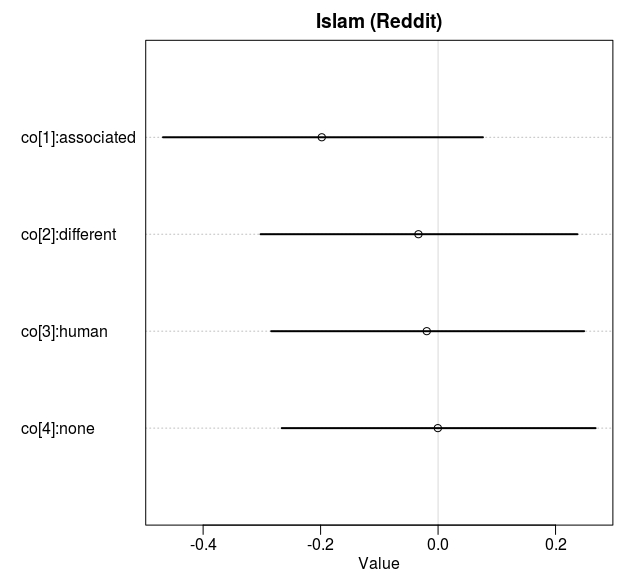
\includegraphics[width=8cm]{../images/islamCoeffs.jpeg}
\end{center}

\normalsize

While muslim words were unusual in the sense that the disparity between
associated attributes and others is stronger, the evidence is still not
conclusive. This is because the variation even within islam-related
words is large enough (and sample sizes sufficiently small) for all the
highest posterior density invervals to still include zeros.

So, it seems, taking a closer look does seem to make a difference. The
question is, what happens if we do take a close look at the level of
protected words?

\chapter{Protected-word level
analysis}\label{protected-word-level-analysis}

\section{Model structure and
assumptions}\label{model-structure-and-assumptions}

Let's turn then to data analysis that takes a look at protected words
separately. This time for each combination of a protected word and a
connection status we will have a separate mean cosine distance estimate,
each coming with its own highest posterior density interval. This means
we will use indices that are result from all such combinations (and then
we will split them up in the model precis to build visualisation, feel
free to look at the \texttt{visualiseStats.R} script for details).

\vspace{1mm} \footnotesize

\begin{Shaded}
\begin{Highlighting}[]
\KeywordTok{options}\NormalTok{(}\DataTypeTok{buildtools.check =} \ControlFlowTok{function}\NormalTok{(action) }\OtherTok{TRUE}\NormalTok{ ) }\CommentTok{#removes install pop-up request}
\NormalTok{religion}\OperatorTok{$}\NormalTok{pwFactor <-}\StringTok{ }\KeywordTok{factor}\NormalTok{(}\KeywordTok{paste0}\NormalTok{(religion}\OperatorTok{$}\NormalTok{protectedWord, }\StringTok{"-"}\NormalTok{, religion}\OperatorTok{$}\NormalTok{connection))}
\NormalTok{religion}\OperatorTok{$}\NormalTok{pwIndex <-}\StringTok{ }\KeywordTok{as.integer}\NormalTok{(religion}\OperatorTok{$}\NormalTok{pwFactor)}

\NormalTok{religionSeparate <-}\StringTok{ }\KeywordTok{ulam}\NormalTok{(}
  \KeywordTok{alist}\NormalTok{(}
\NormalTok{    cosineDistance }\OperatorTok{~}\StringTok{ }\KeywordTok{dnorm}\NormalTok{(mu,sigma),}
\NormalTok{    mu <-}\StringTok{ }\NormalTok{c[pwIndex],}
\NormalTok{    c[pwIndex] }\OperatorTok{~}\StringTok{ }\KeywordTok{dnorm}\NormalTok{(}\DecValTok{1}\NormalTok{,.}\DecValTok{5}\NormalTok{),}
\NormalTok{    sigma }\OperatorTok{~}\StringTok{ }\KeywordTok{dcauchy}\NormalTok{(}\DecValTok{0}\NormalTok{,}\DecValTok{1}\NormalTok{)}
\NormalTok{  ),}
  \DataTypeTok{data =}\NormalTok{ religion,}
  \DataTypeTok{chains=}\DecValTok{2}\NormalTok{ , }\DataTypeTok{iter=}\DecValTok{10000}\NormalTok{ , }\DataTypeTok{warmup=}\DecValTok{1000}\NormalTok{,}
  \DataTypeTok{start=}\KeywordTok{list}\NormalTok{(}\DataTypeTok{no =} \DecValTok{1}\NormalTok{, }\DataTypeTok{a =} \DecValTok{0}\NormalTok{, }\DataTypeTok{d =} \DecValTok{0}\NormalTok{, }\DataTypeTok{sigma=} \FloatTok{.3}\NormalTok{), }\DataTypeTok{log_lik =}  \OtherTok{TRUE}
\NormalTok{)}
\end{Highlighting}
\end{Shaded}

\normalsize

\noindent Let's see if the individualized model does better than the
previous models in light of WAIC which does add penalty for the number
of parameters.

\vspace{1mm} \footnotesize

\begin{Shaded}
\begin{Highlighting}[]
\NormalTok{compareBaselineCoefsSeparate<-}\StringTok{ }\KeywordTok{readRDS}\NormalTok{(}\StringTok{"../datasets/compareBaselineCoefsSeparate.rds"}\NormalTok{)}
\NormalTok{compareBaselineCoefsSeparate}
\end{Highlighting}
\end{Shaded}

\begin{verbatim}
##                   WAIC SE dWAIC dSE pWAIC weight
## religionSeparate -2400 93     0  NA    60      1
## religionCoefs    -2328 93    72  29    20      0
## religionBaseline -2283 95   117  37    16      0
\end{verbatim}

\normalsize

\section{Protected classes in Reddit and Google
embeddings}\label{protected-classes-in-reddit-and-google-embeddings}

It seems that we do want to prefer this model, despite its relative
complication. Now, what does it tell us about the protected words? Let's
visualise the predicted means together with 89\% highest posterior
density intervals.

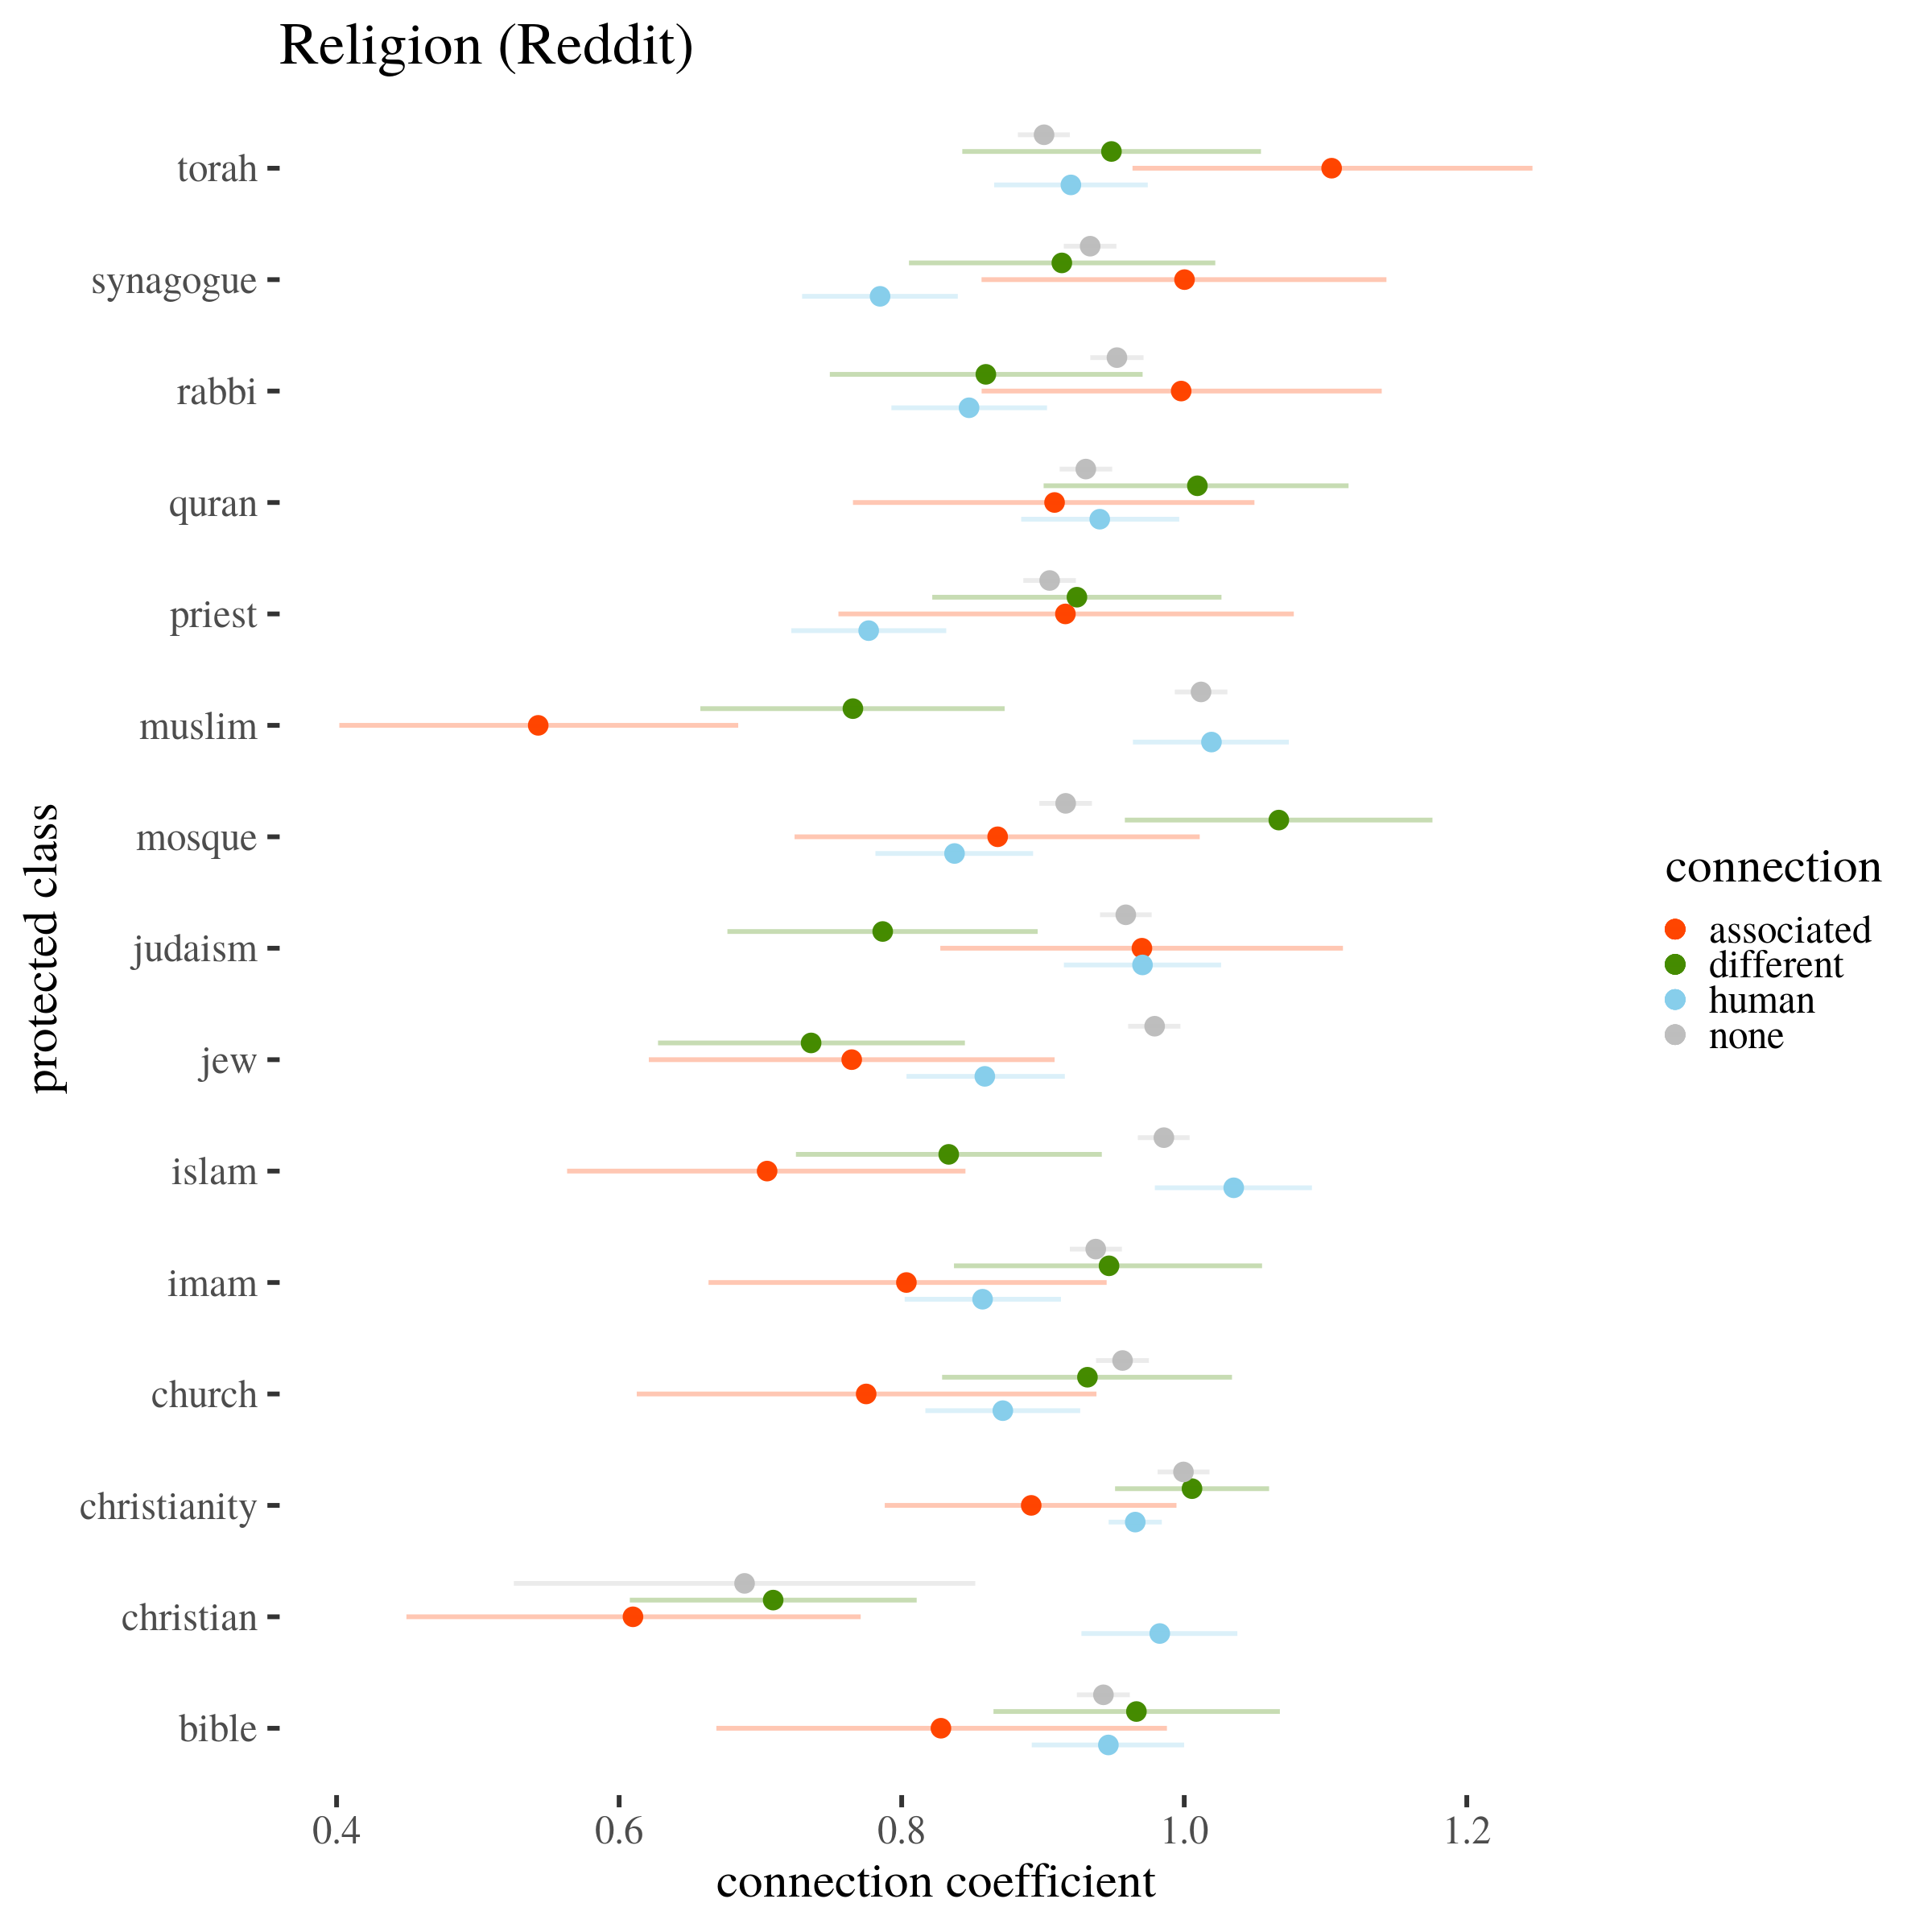
\includegraphics[width=14cm]{../images/visReligionReddit.png}

Before we move on, let's perform analogous analyses for the remaining
types of supposed bias: gender and race (the model building is
analogous).

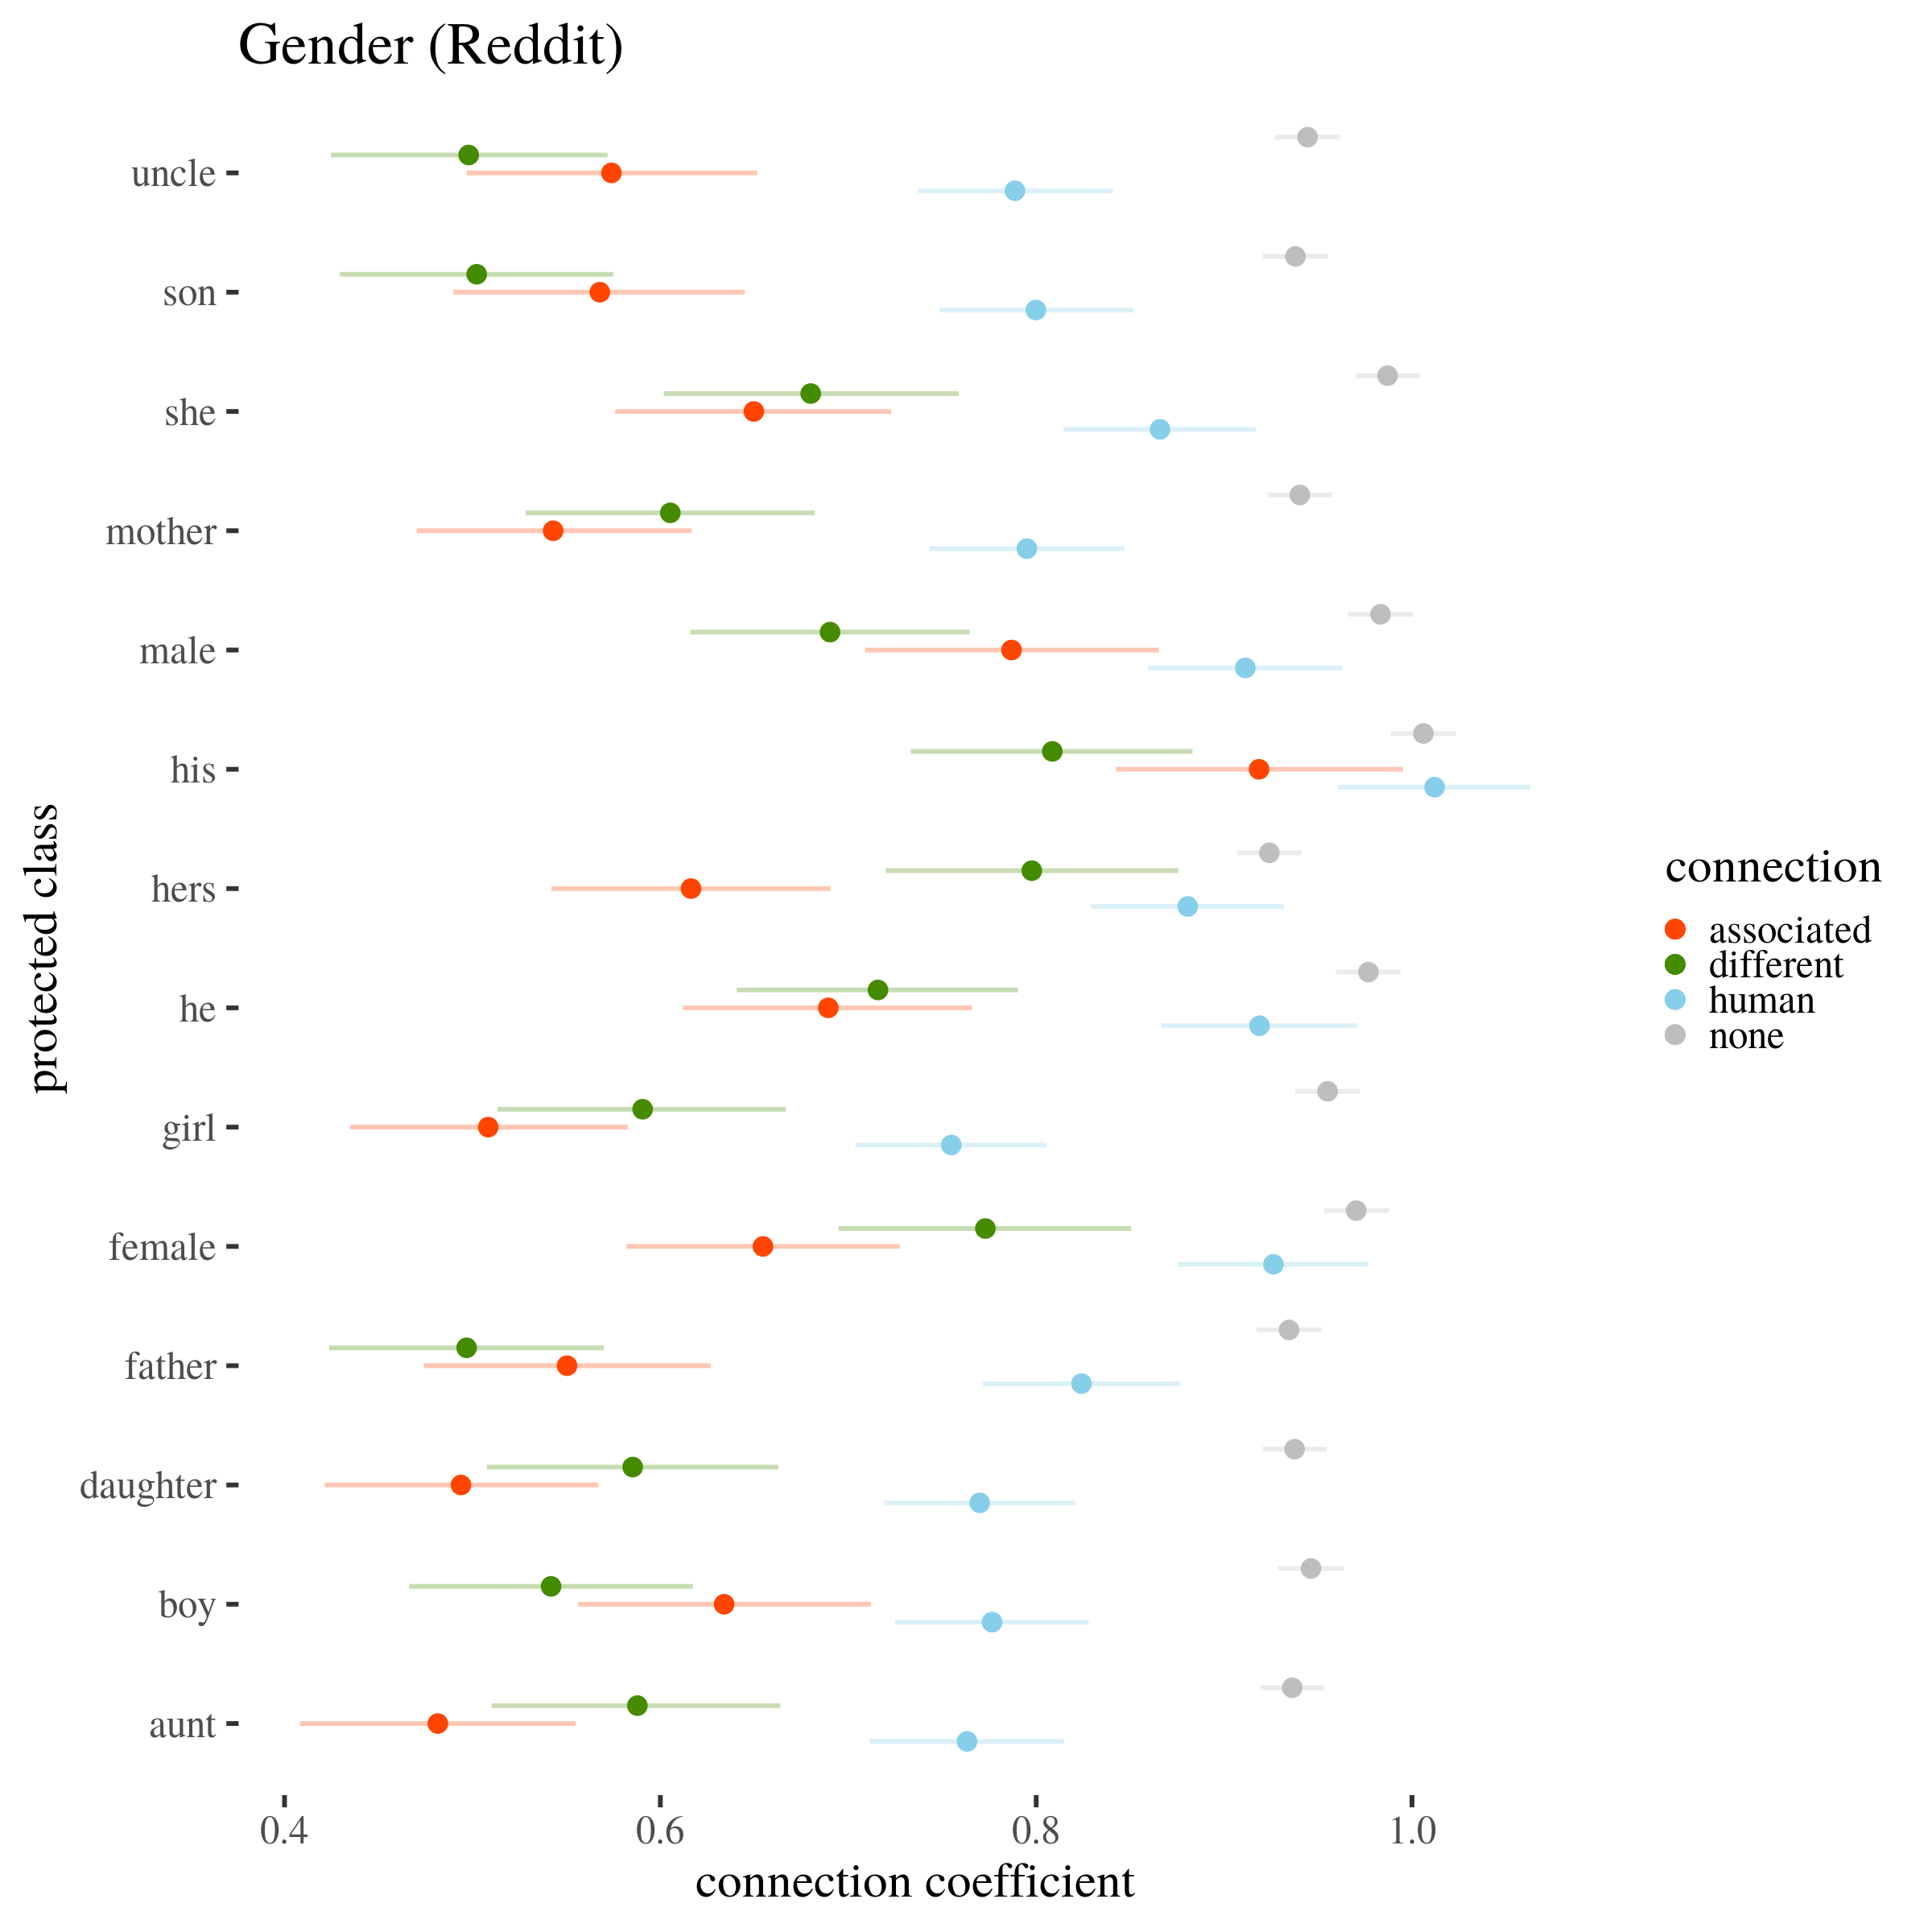
\includegraphics[width=14cm]{../images/visGenderReddit.png}

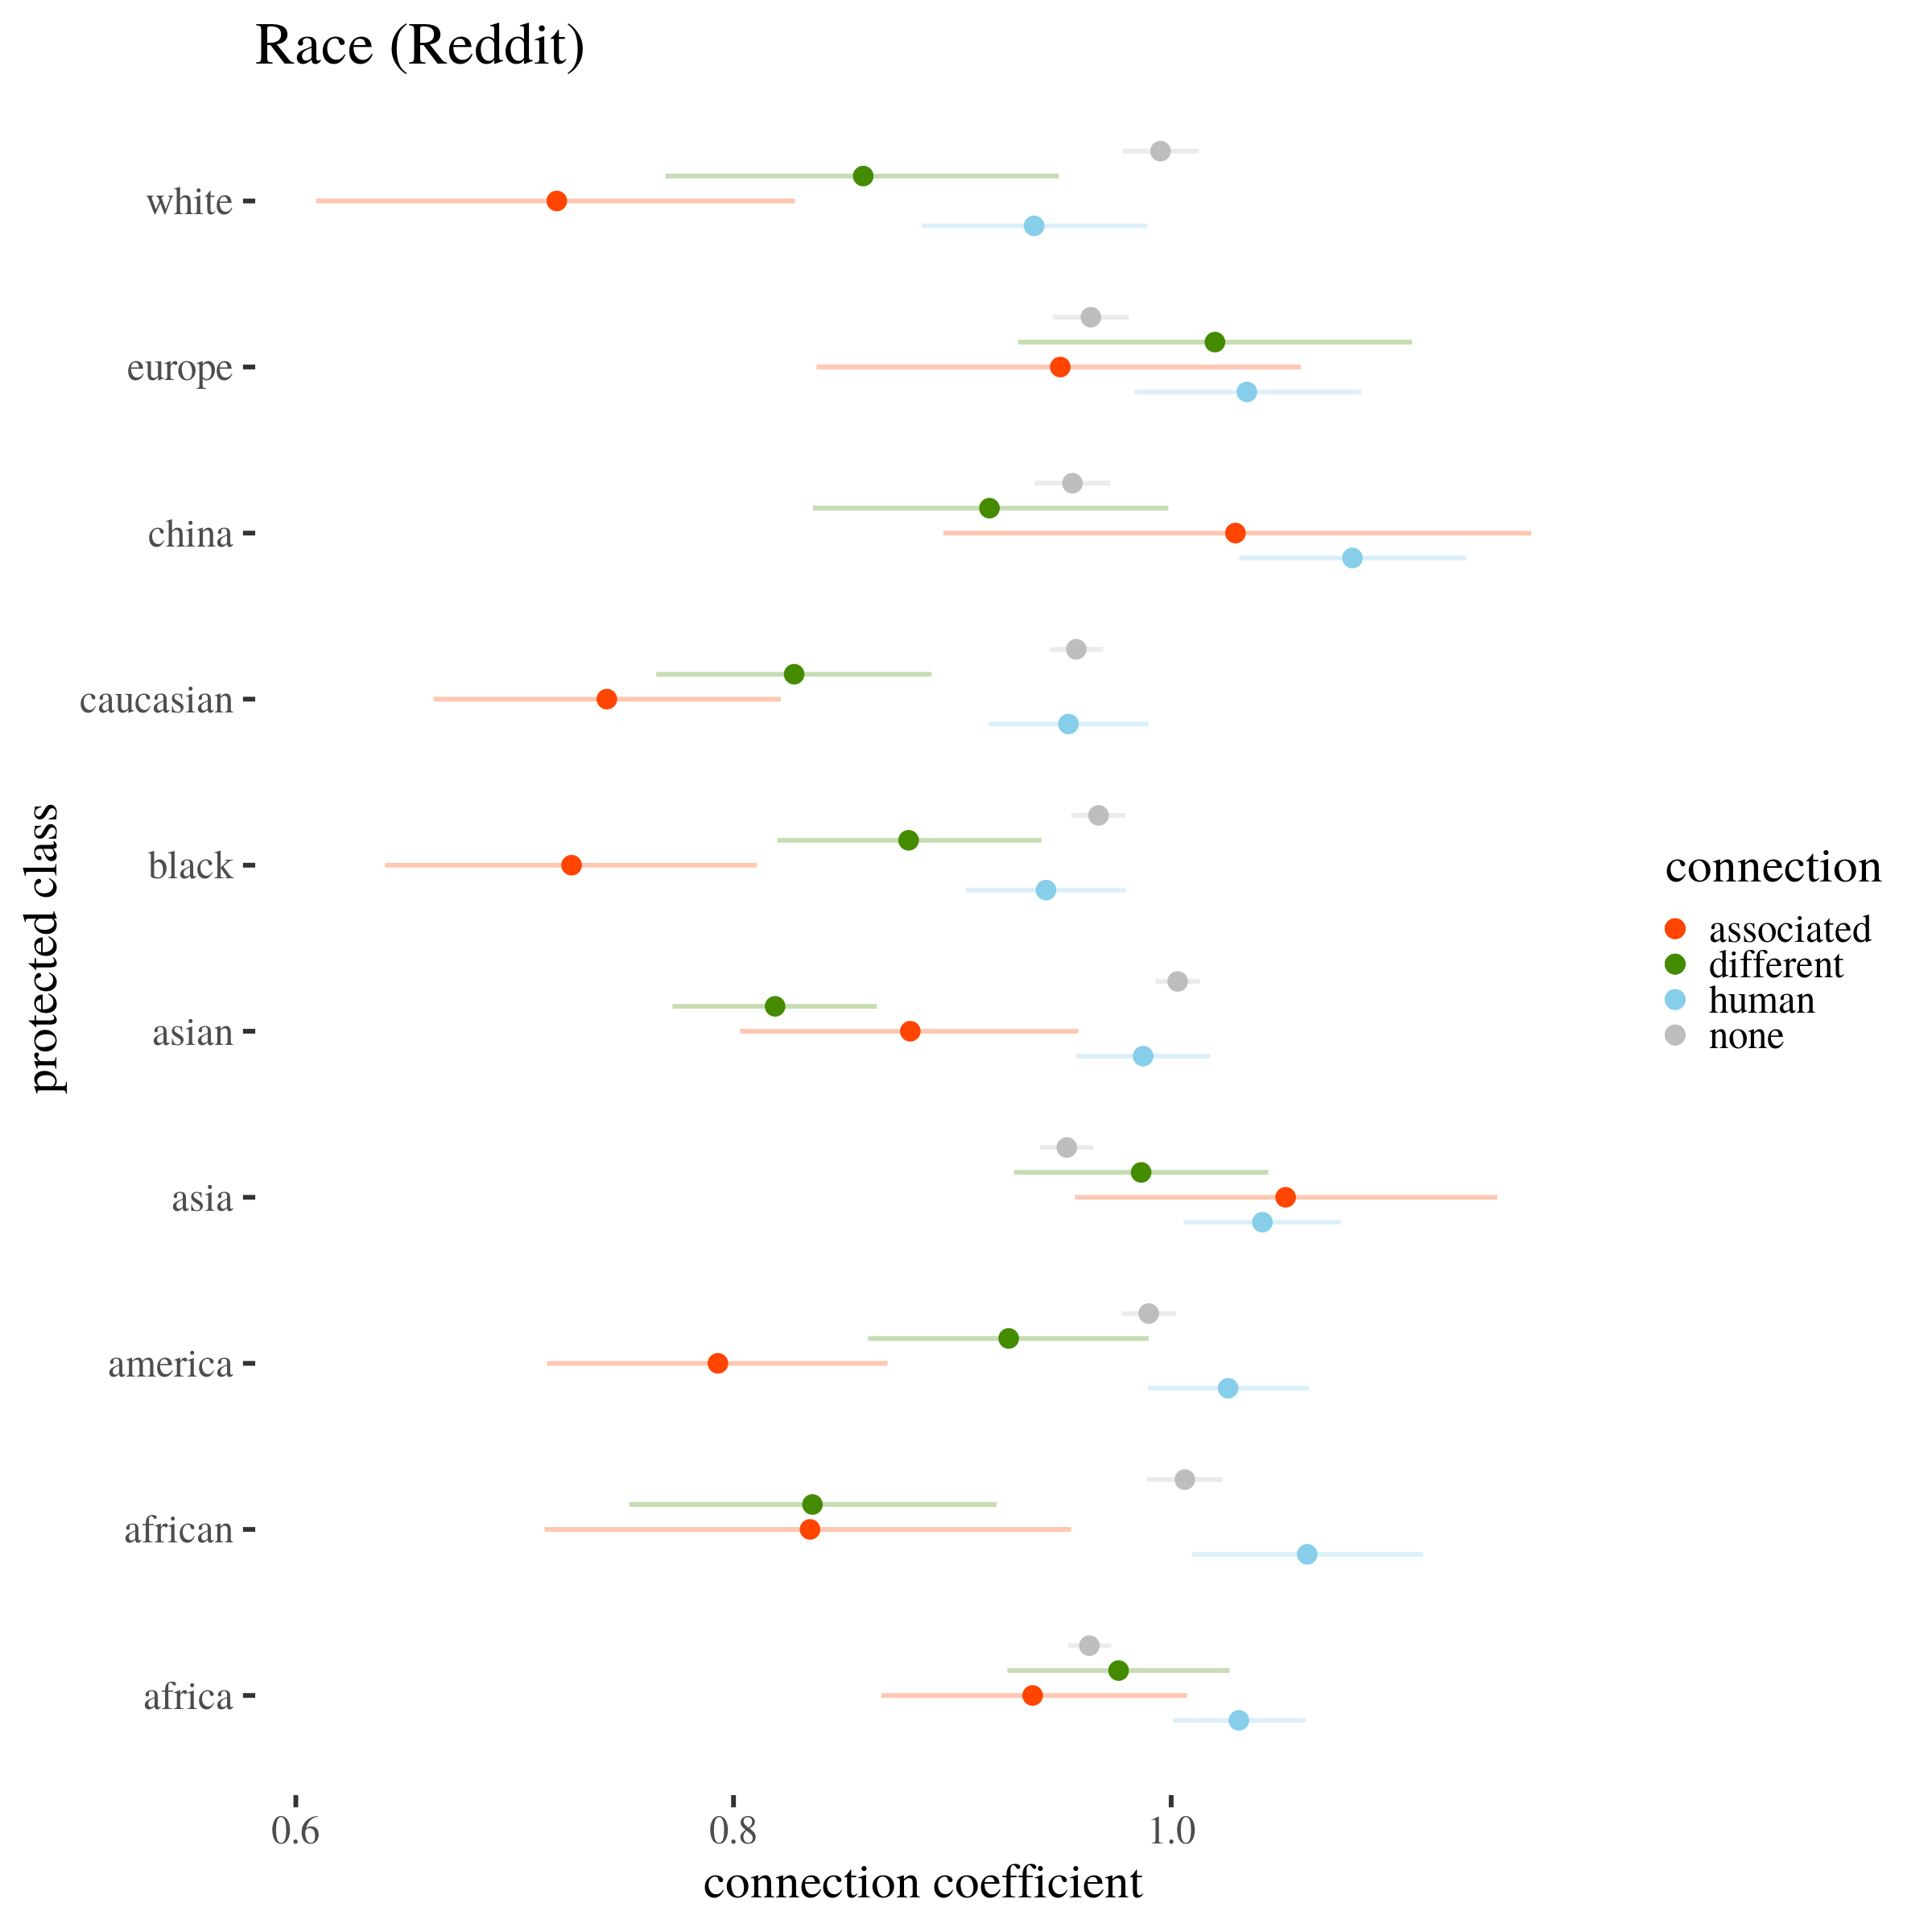
\includegraphics[width=14cm]{../images/visRaceReddit.png}

\todo{Explain where you took the embedding from, cite publications first announcing it.}

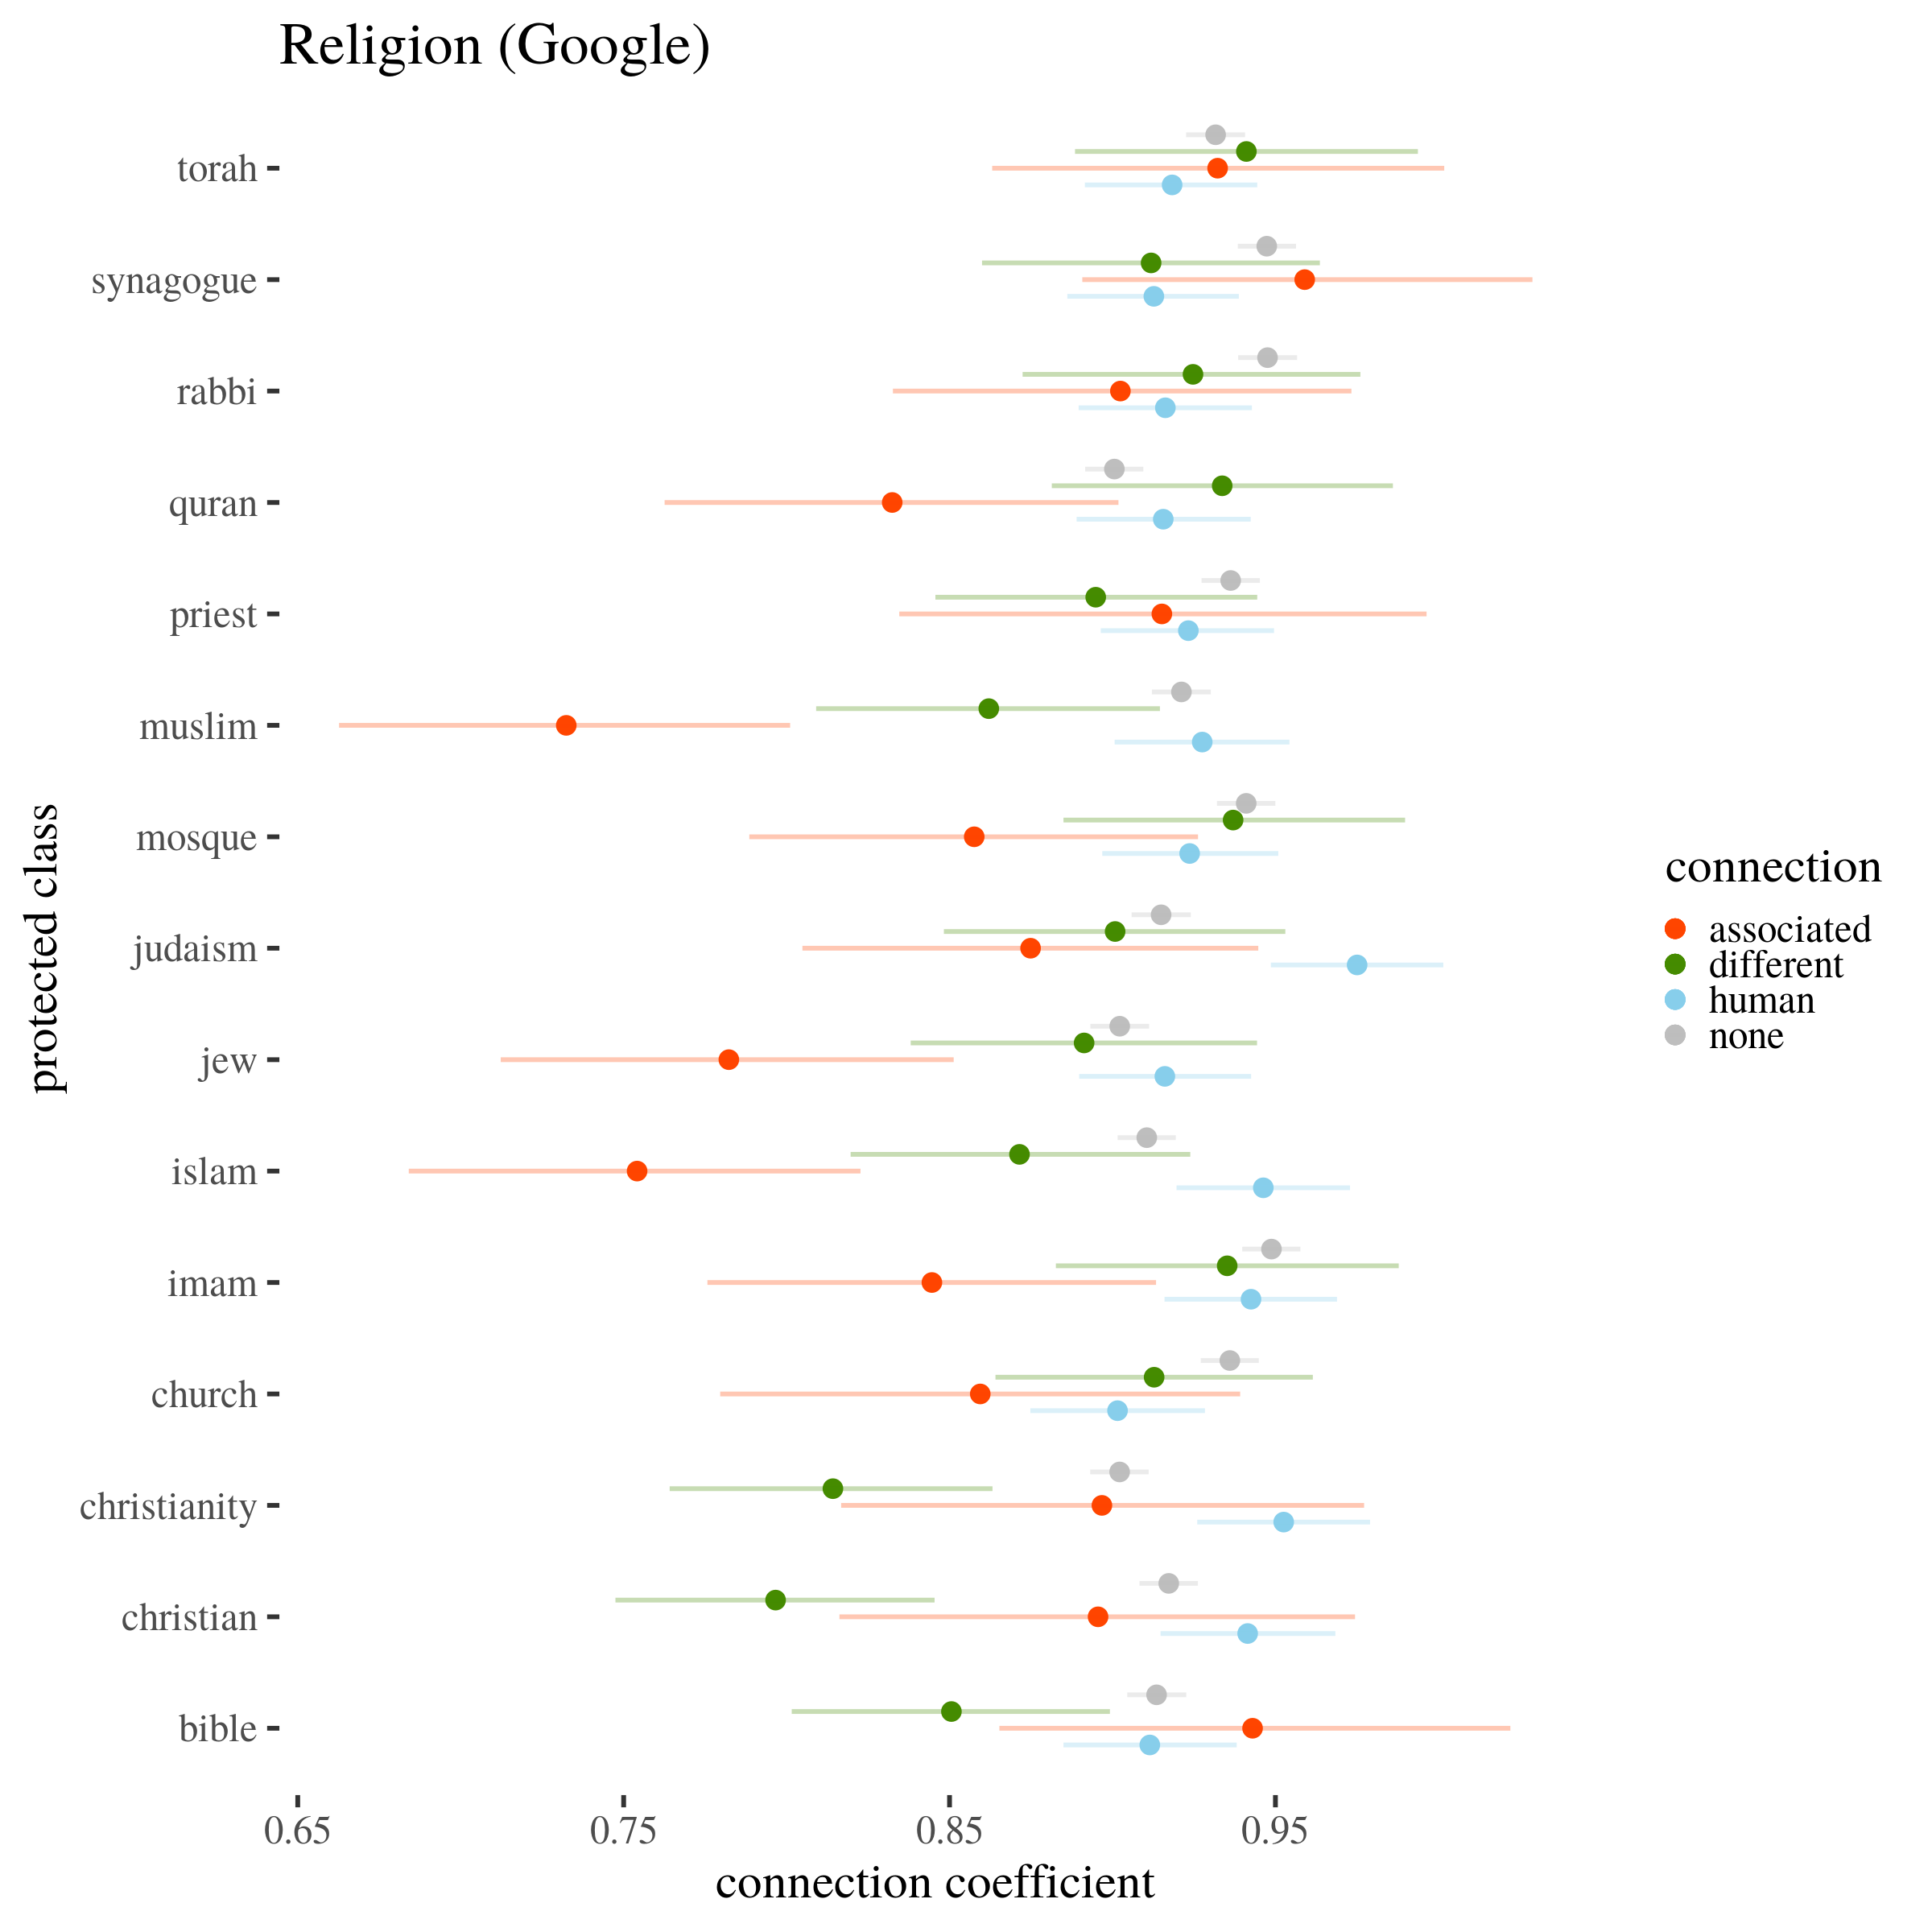
\includegraphics[width=14cm]{../images/visReligionGoogle.png}

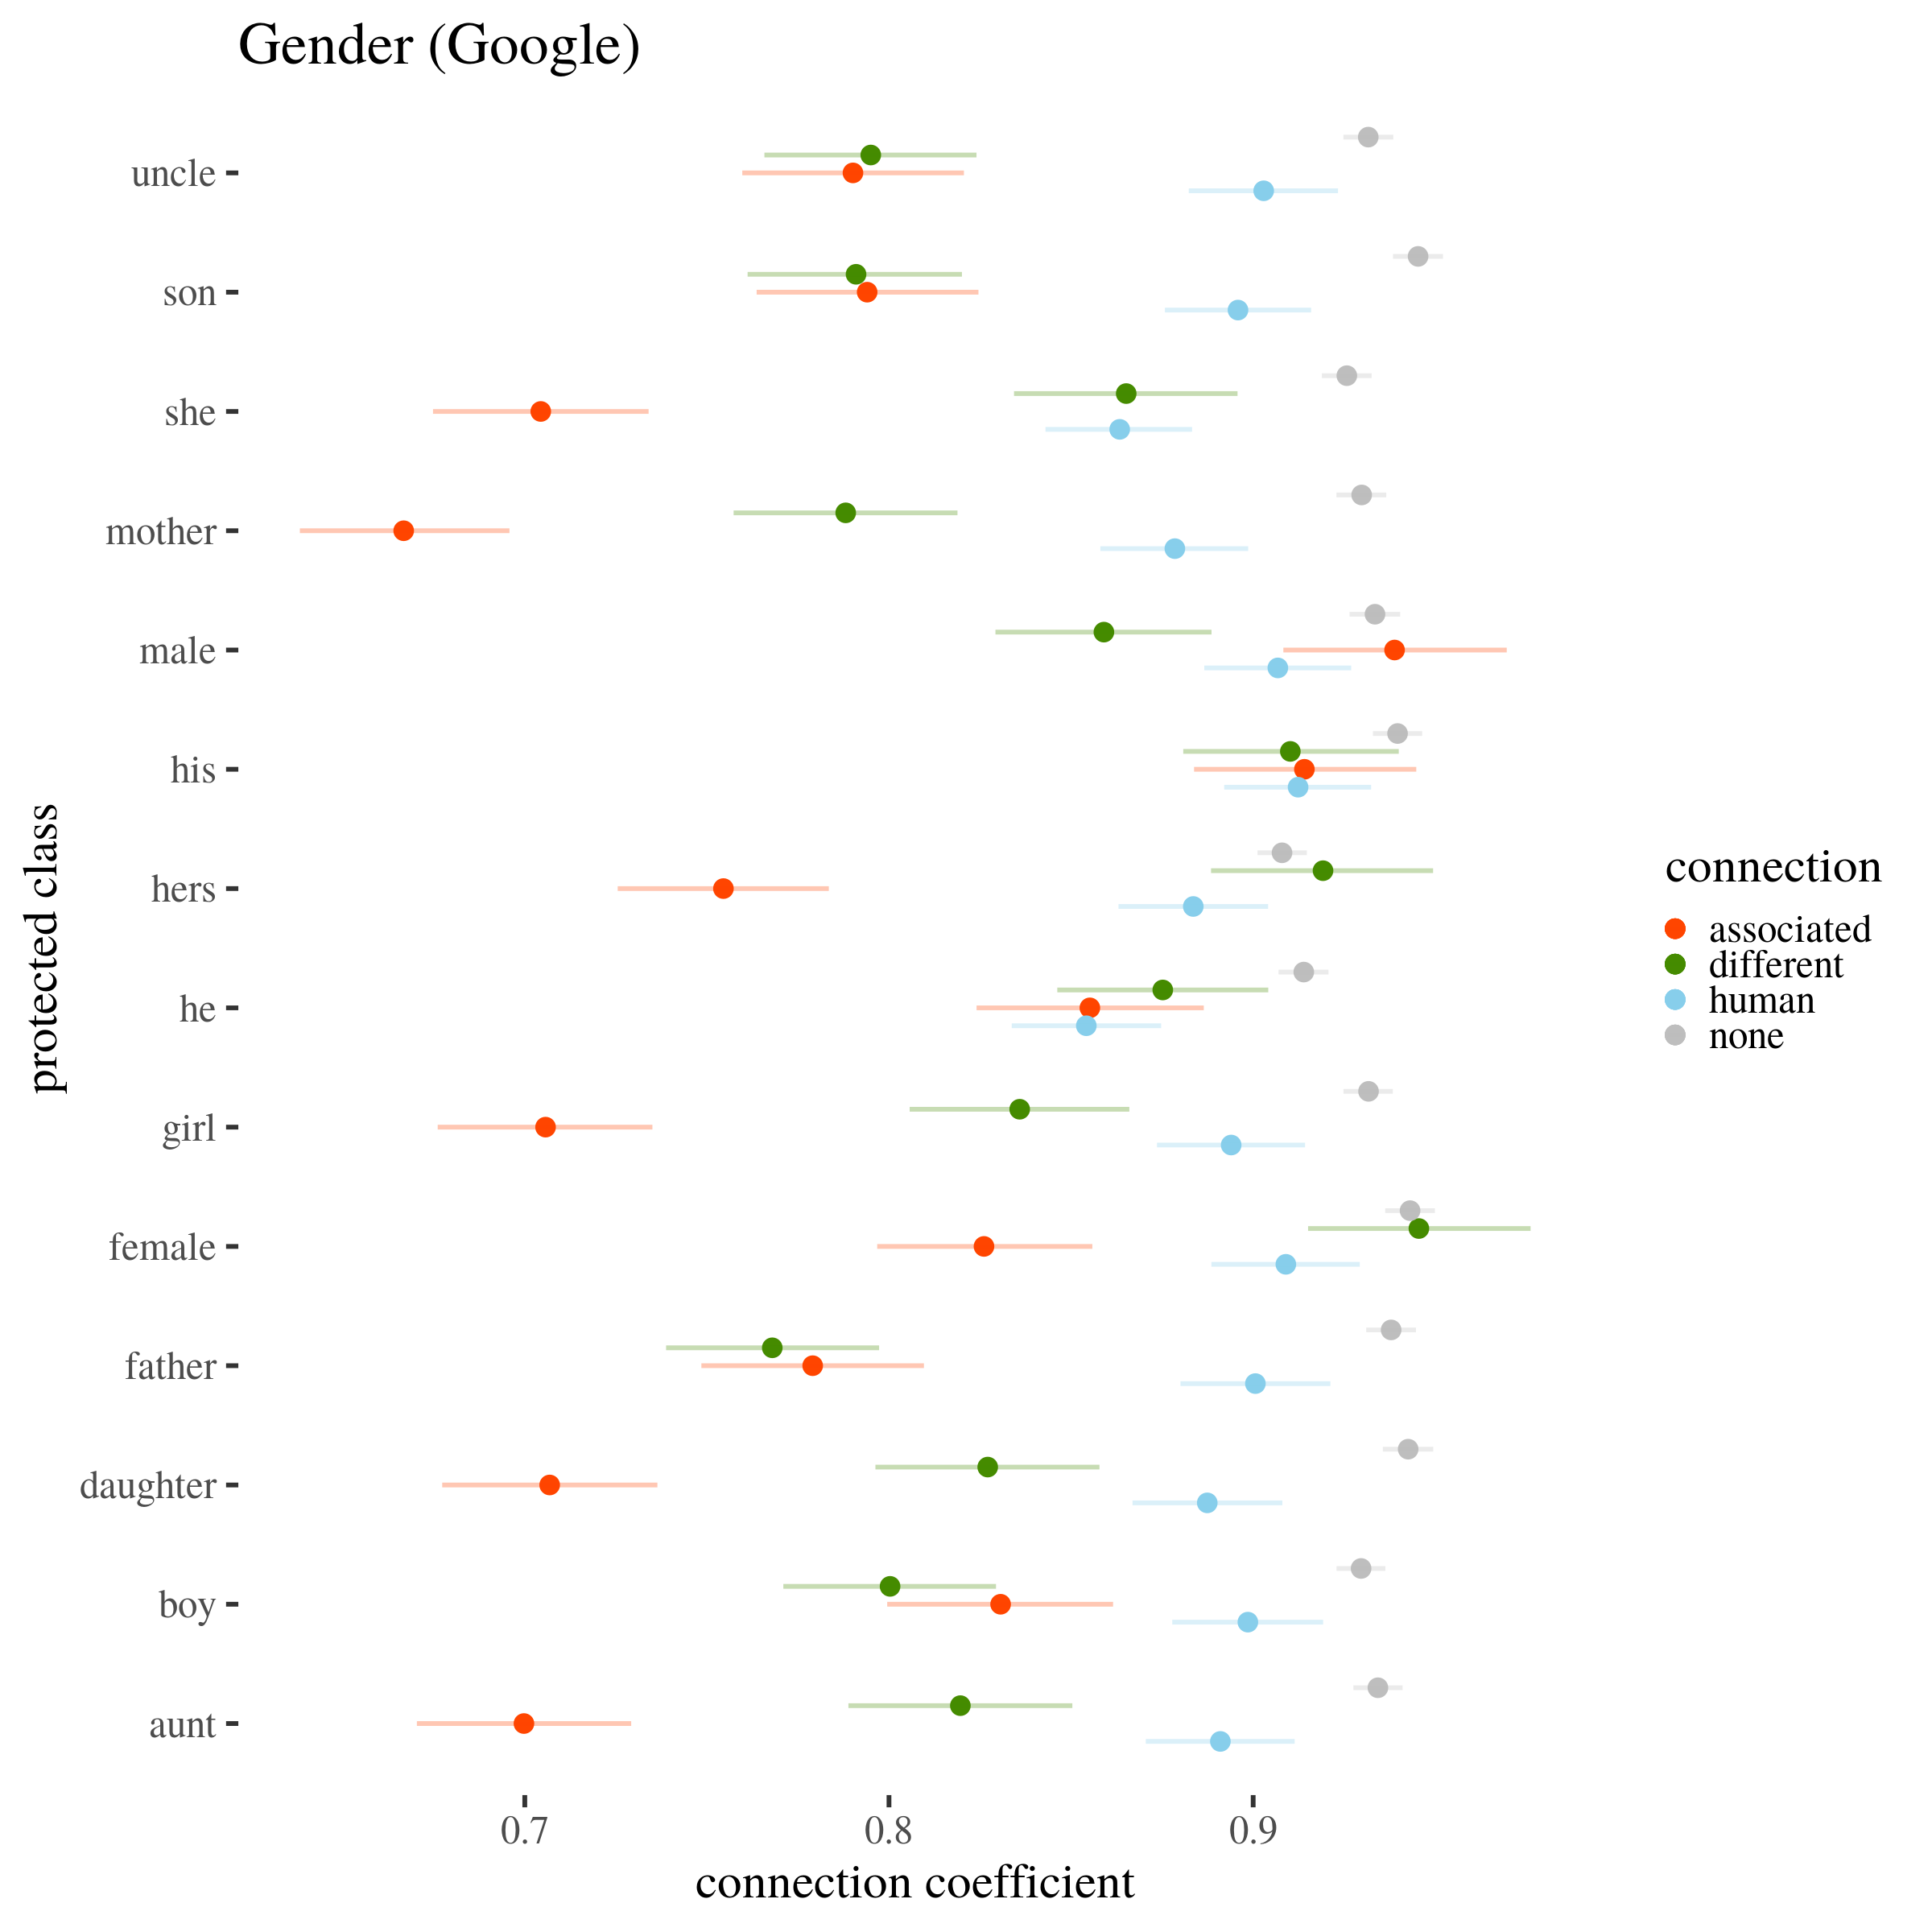
\includegraphics[width=14cm]{../images/visGenderGoogle.png}

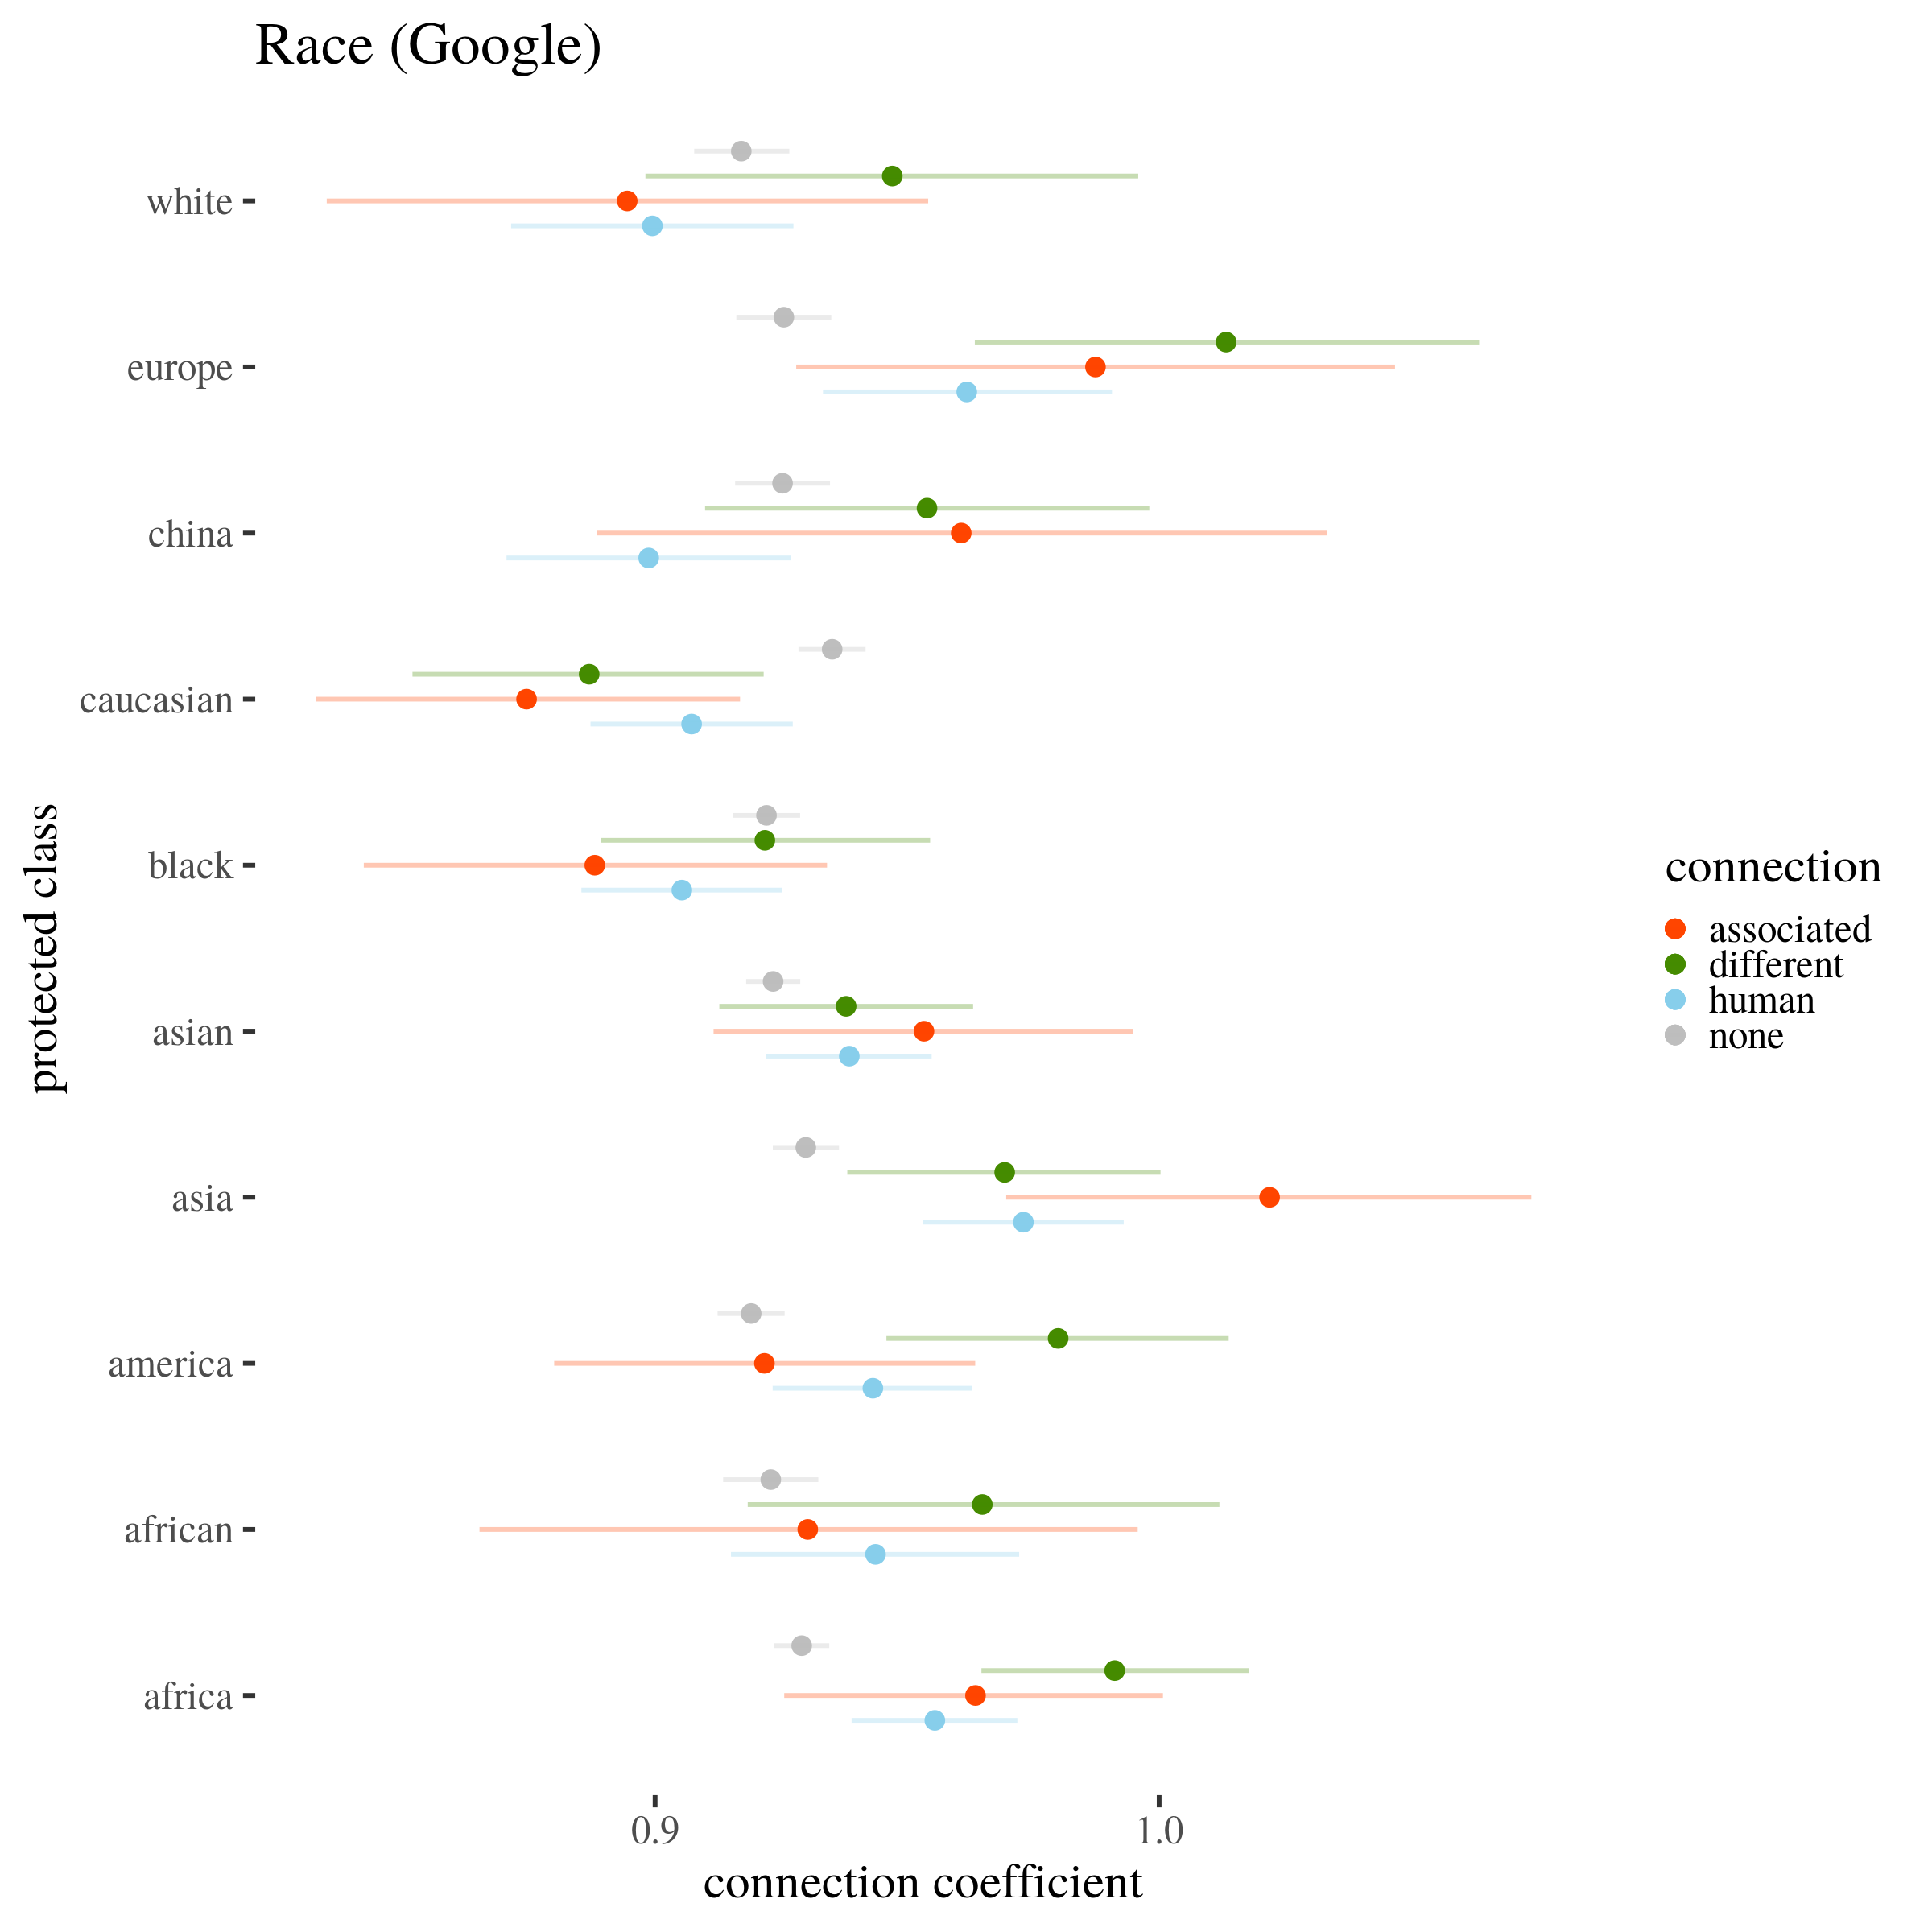
\includegraphics[width=14cm]{../images/visRaceGoogle.png}

\chapter{The role of debiasing}\label{the-role-of-debiasing}

\todo{describe which debiasing you used and how it was advertised in the paper}

\section{Dataset-level coefficients after
debiasing}\label{dataset-level-coefficients-after-debiasing}

First, let's look at coefficient estimated for the whole datasets, as
compared to their estimation prior to debiasing:

\begin{center}
\begin{figure}[!htb]\centering
   \begin{minipage}{0.55\textwidth}
  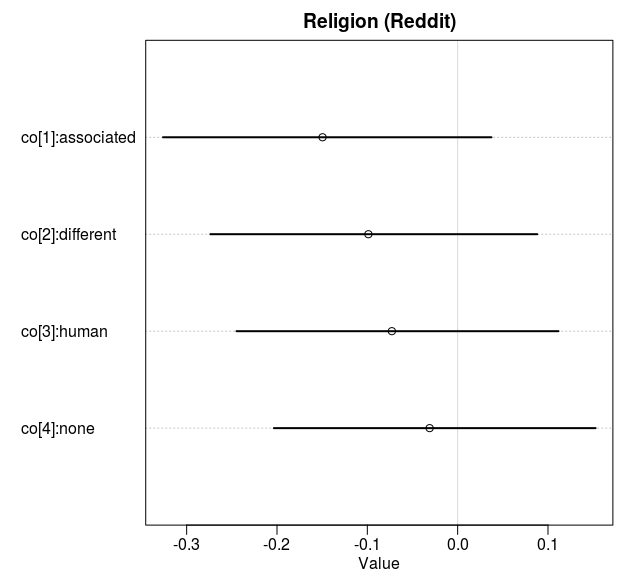
\includegraphics[width=7cm]{../images/religionCoeffs.jpeg}
   \end{minipage}
   \begin {minipage}{0.43\textwidth}
    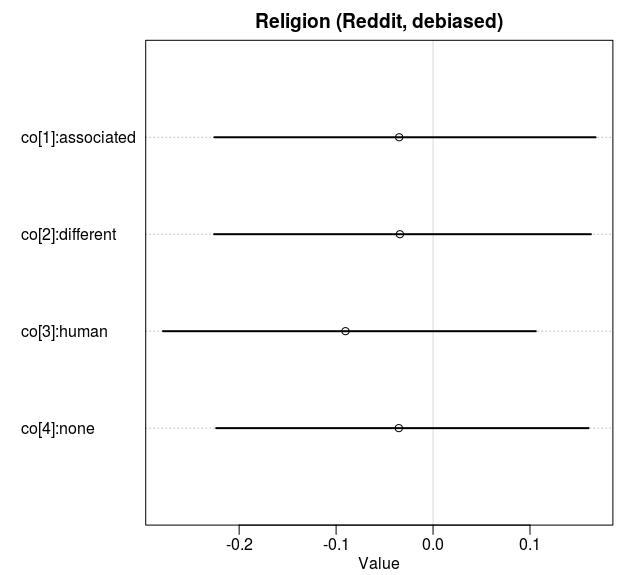
\includegraphics[width=7cm]{../images/debiasedReligionRedditCoeffs.jpeg}
   \end{minipage}
   
   
  \begin{minipage}{0.55\textwidth}
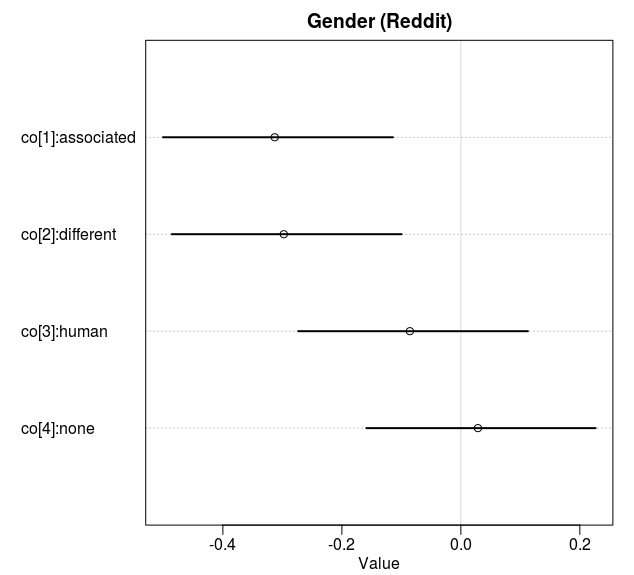
\includegraphics[width=7cm]{../images/genderCoeffs.jpeg}
\end{minipage}
   \begin {minipage}{0.43\textwidth}
    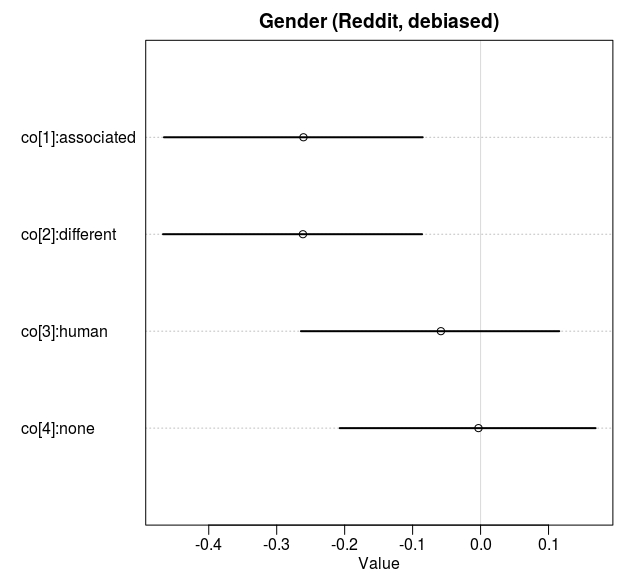
\includegraphics[width=7cm]{../images/debiasedGenderRedditCoeffs.jpeg}
   \end{minipage}
   
   
   
   
  \begin{minipage}{0.55\textwidth}
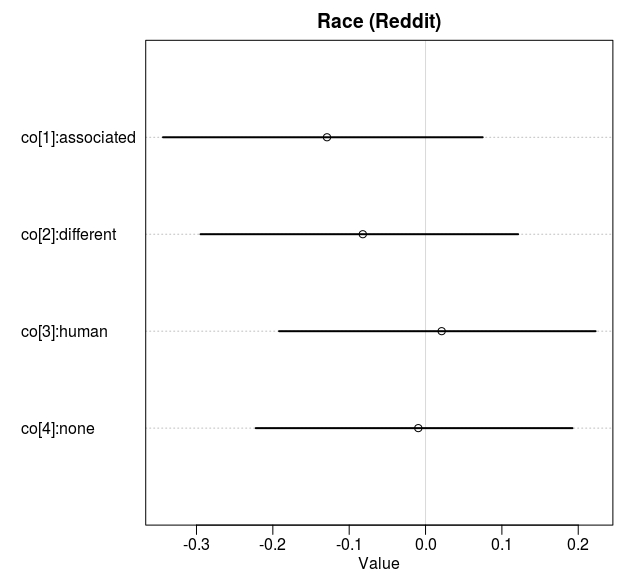
\includegraphics[width=7cm]{../images/raceCoeffs.jpeg}
\end{minipage}
   \begin {minipage}{0.43\textwidth}
    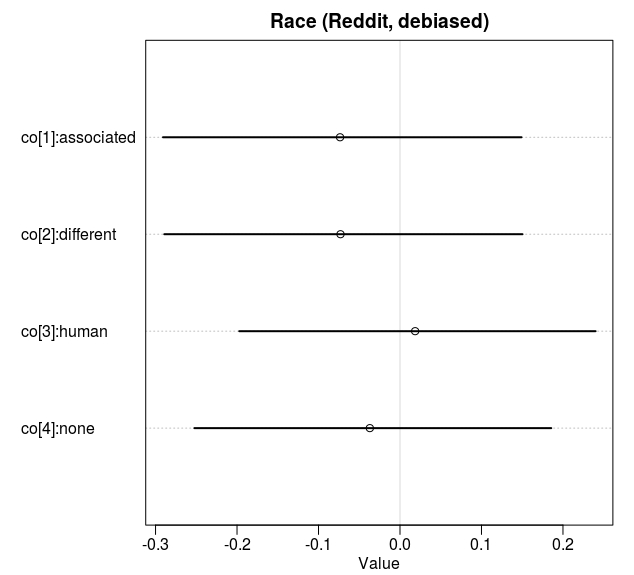
\includegraphics[width=7cm]{../images/debiasedRaceRedditCoeffs.jpeg}
   \end{minipage}
\end{figure}

\end{center}

\todo{comment on this}

Some points to discuss:

\begin{itemize}
\item
  humans in religion got closer (should they?)
\item
  change in Gender is really minor, still zero out of HPDI range, note
  how different is very similar
\item
  small improvement in race, at the price of moving neutral terms closer
\end{itemize}

\section{Protected classes after
debiasing}\label{protected-classes-after-debiasing}

Now, perhaps, the effects of debiasing will be better appreciated if we
look at the level of protected words. After all, the hope is, the
situation of extremely ill-positioned protected words have improved?

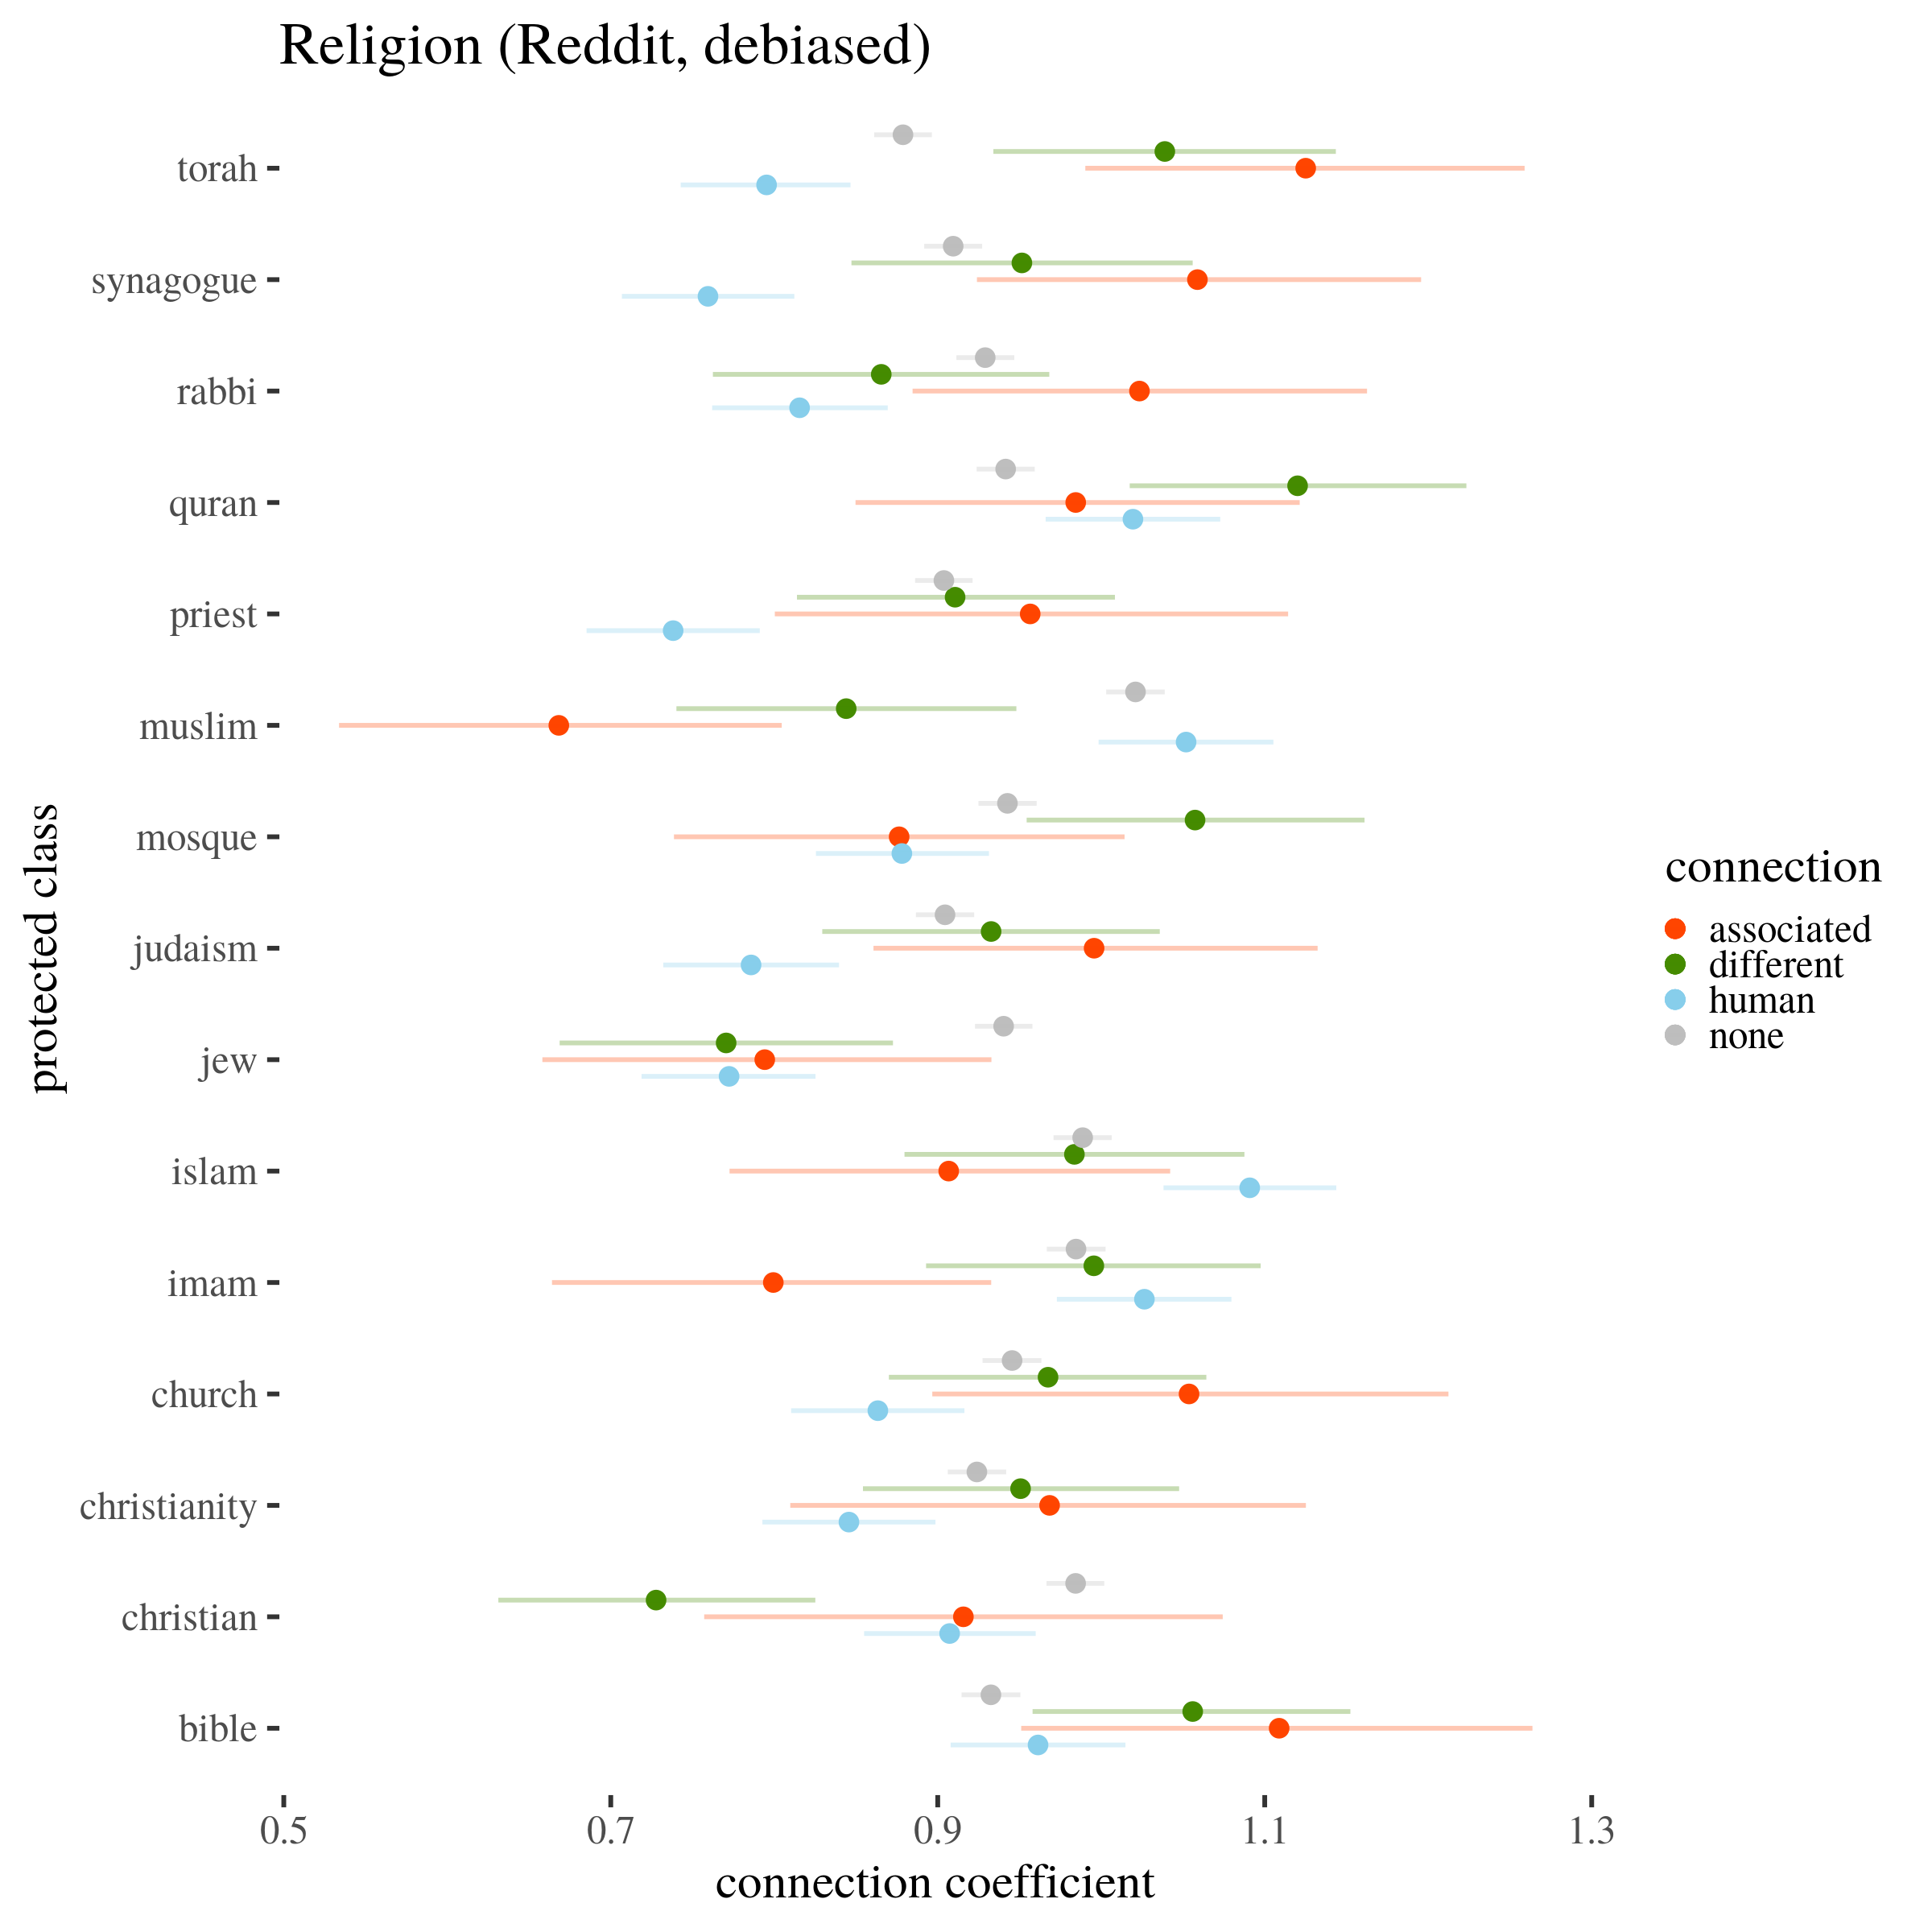
\includegraphics[width=14cm]{../images/visDebReligionReddit.png}

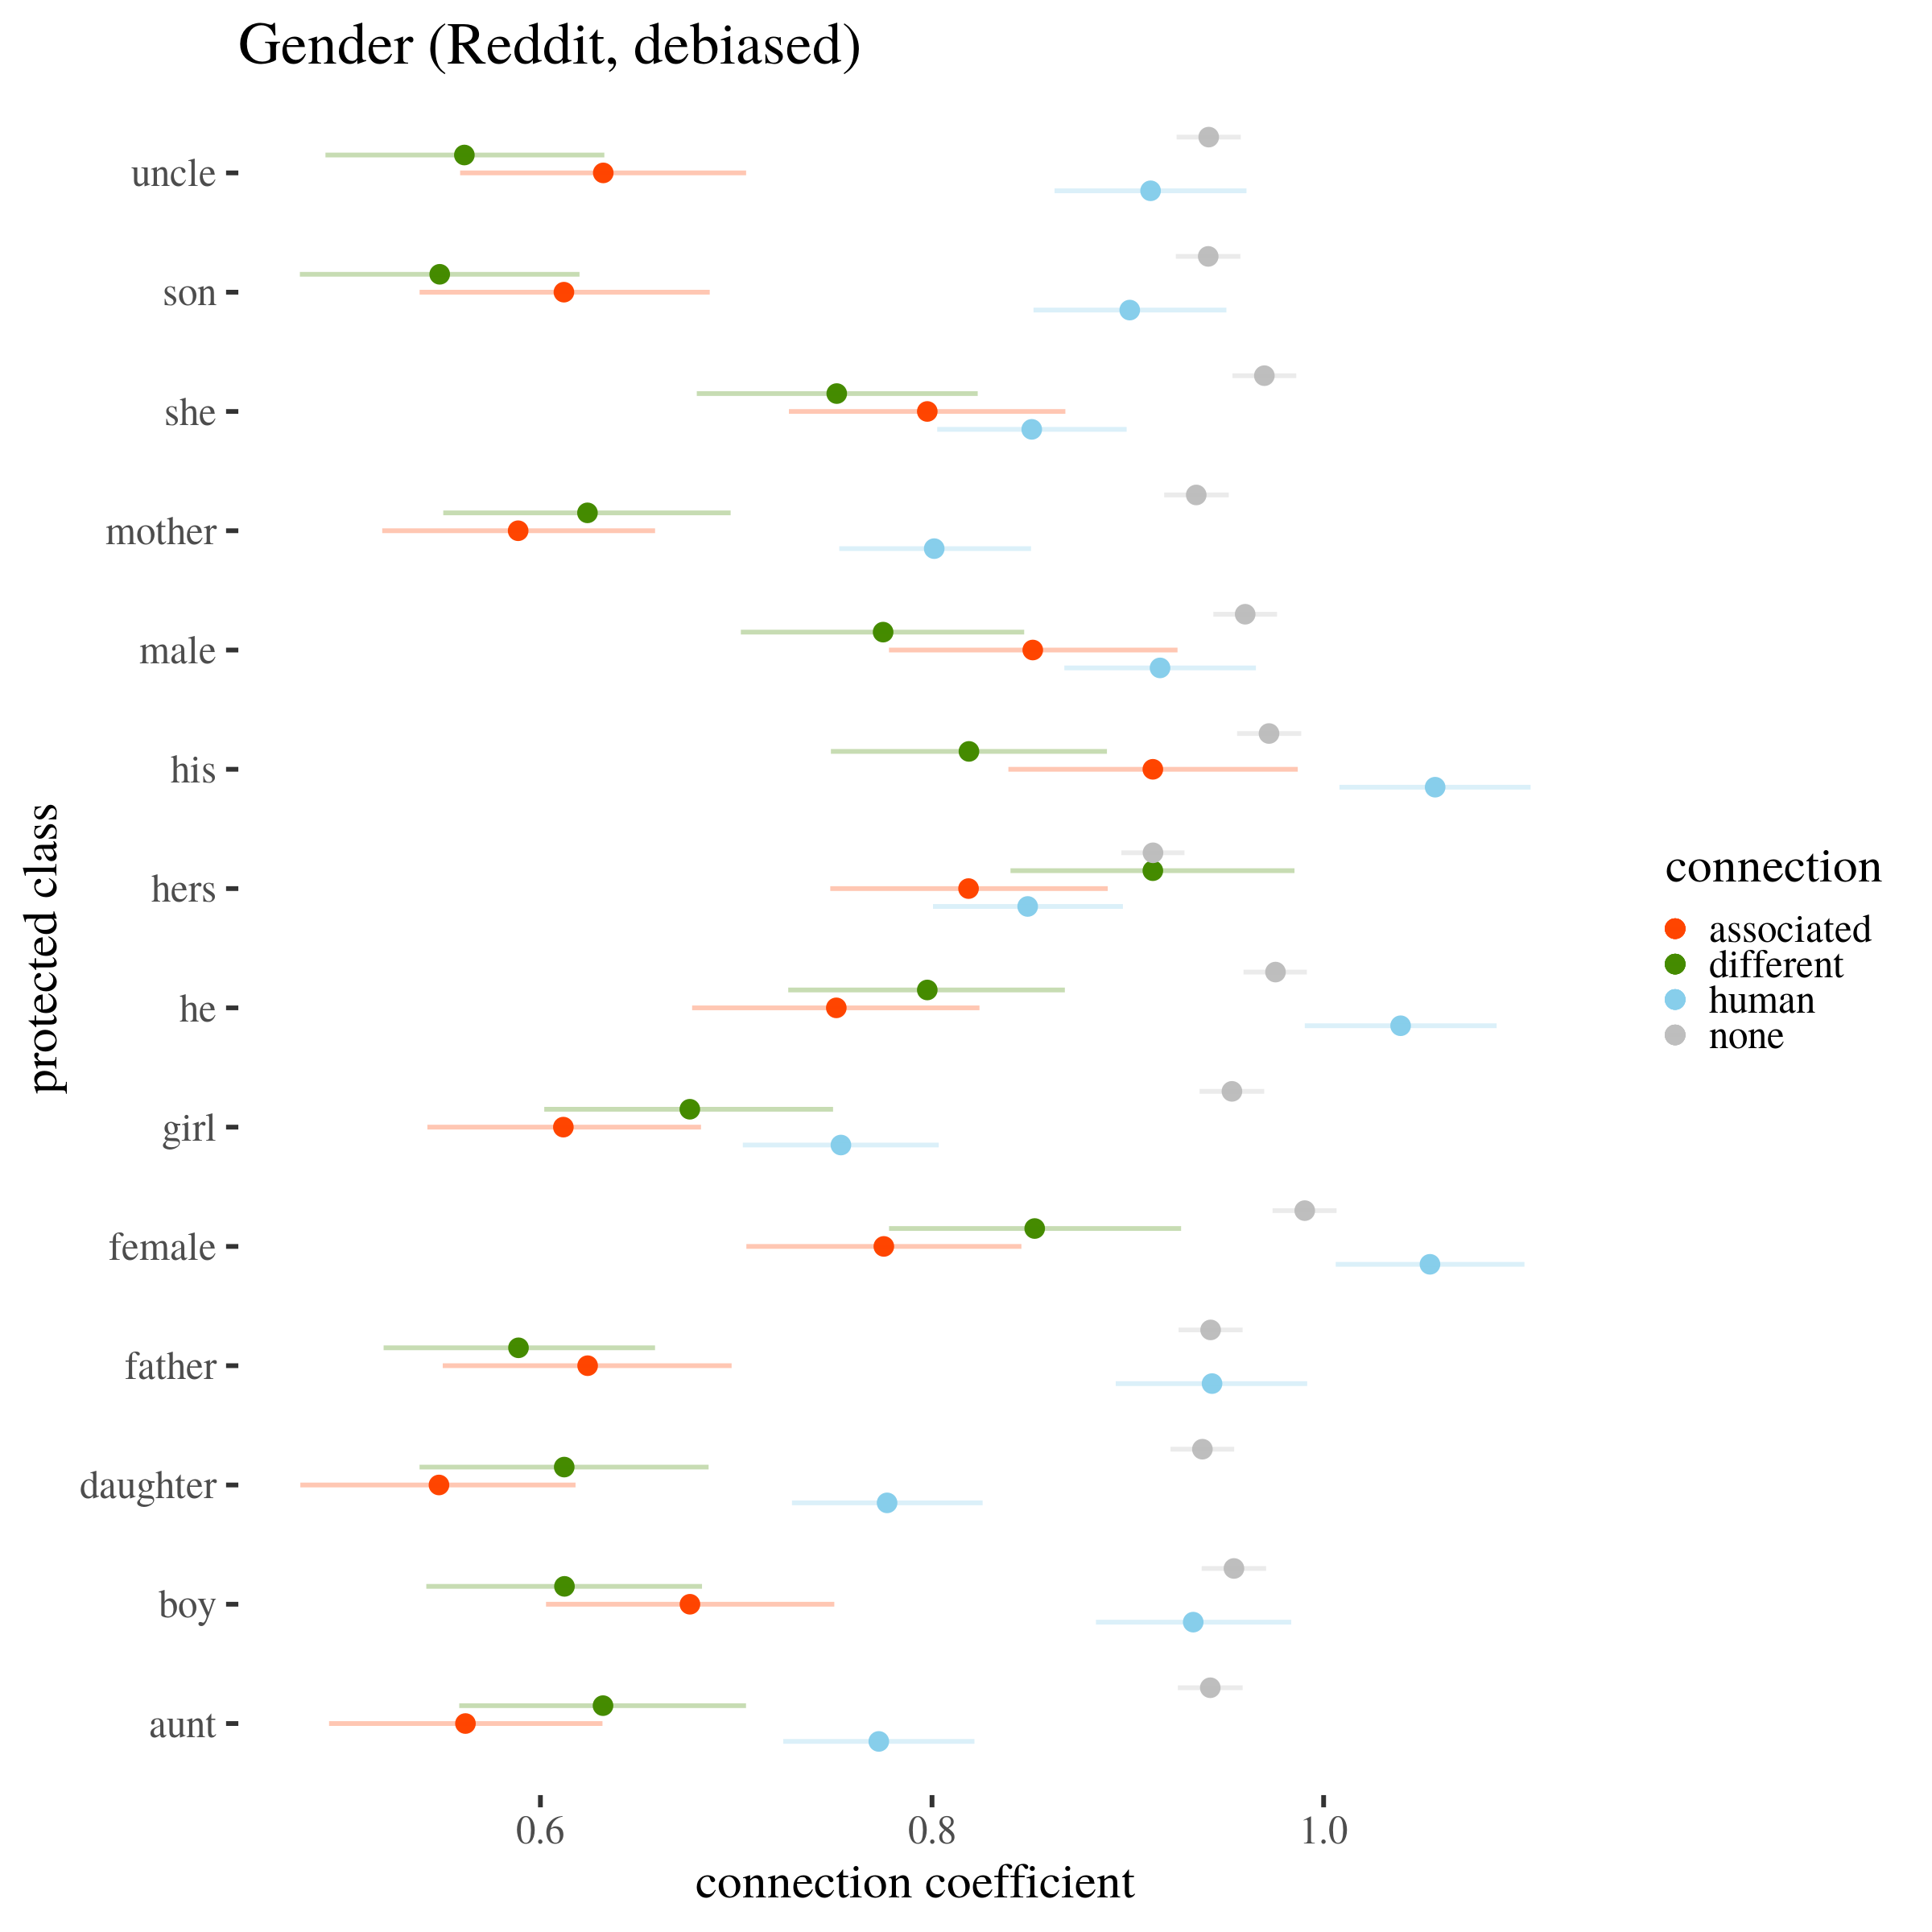
\includegraphics[width=14cm]{../images/visDebGenderReddit.png}

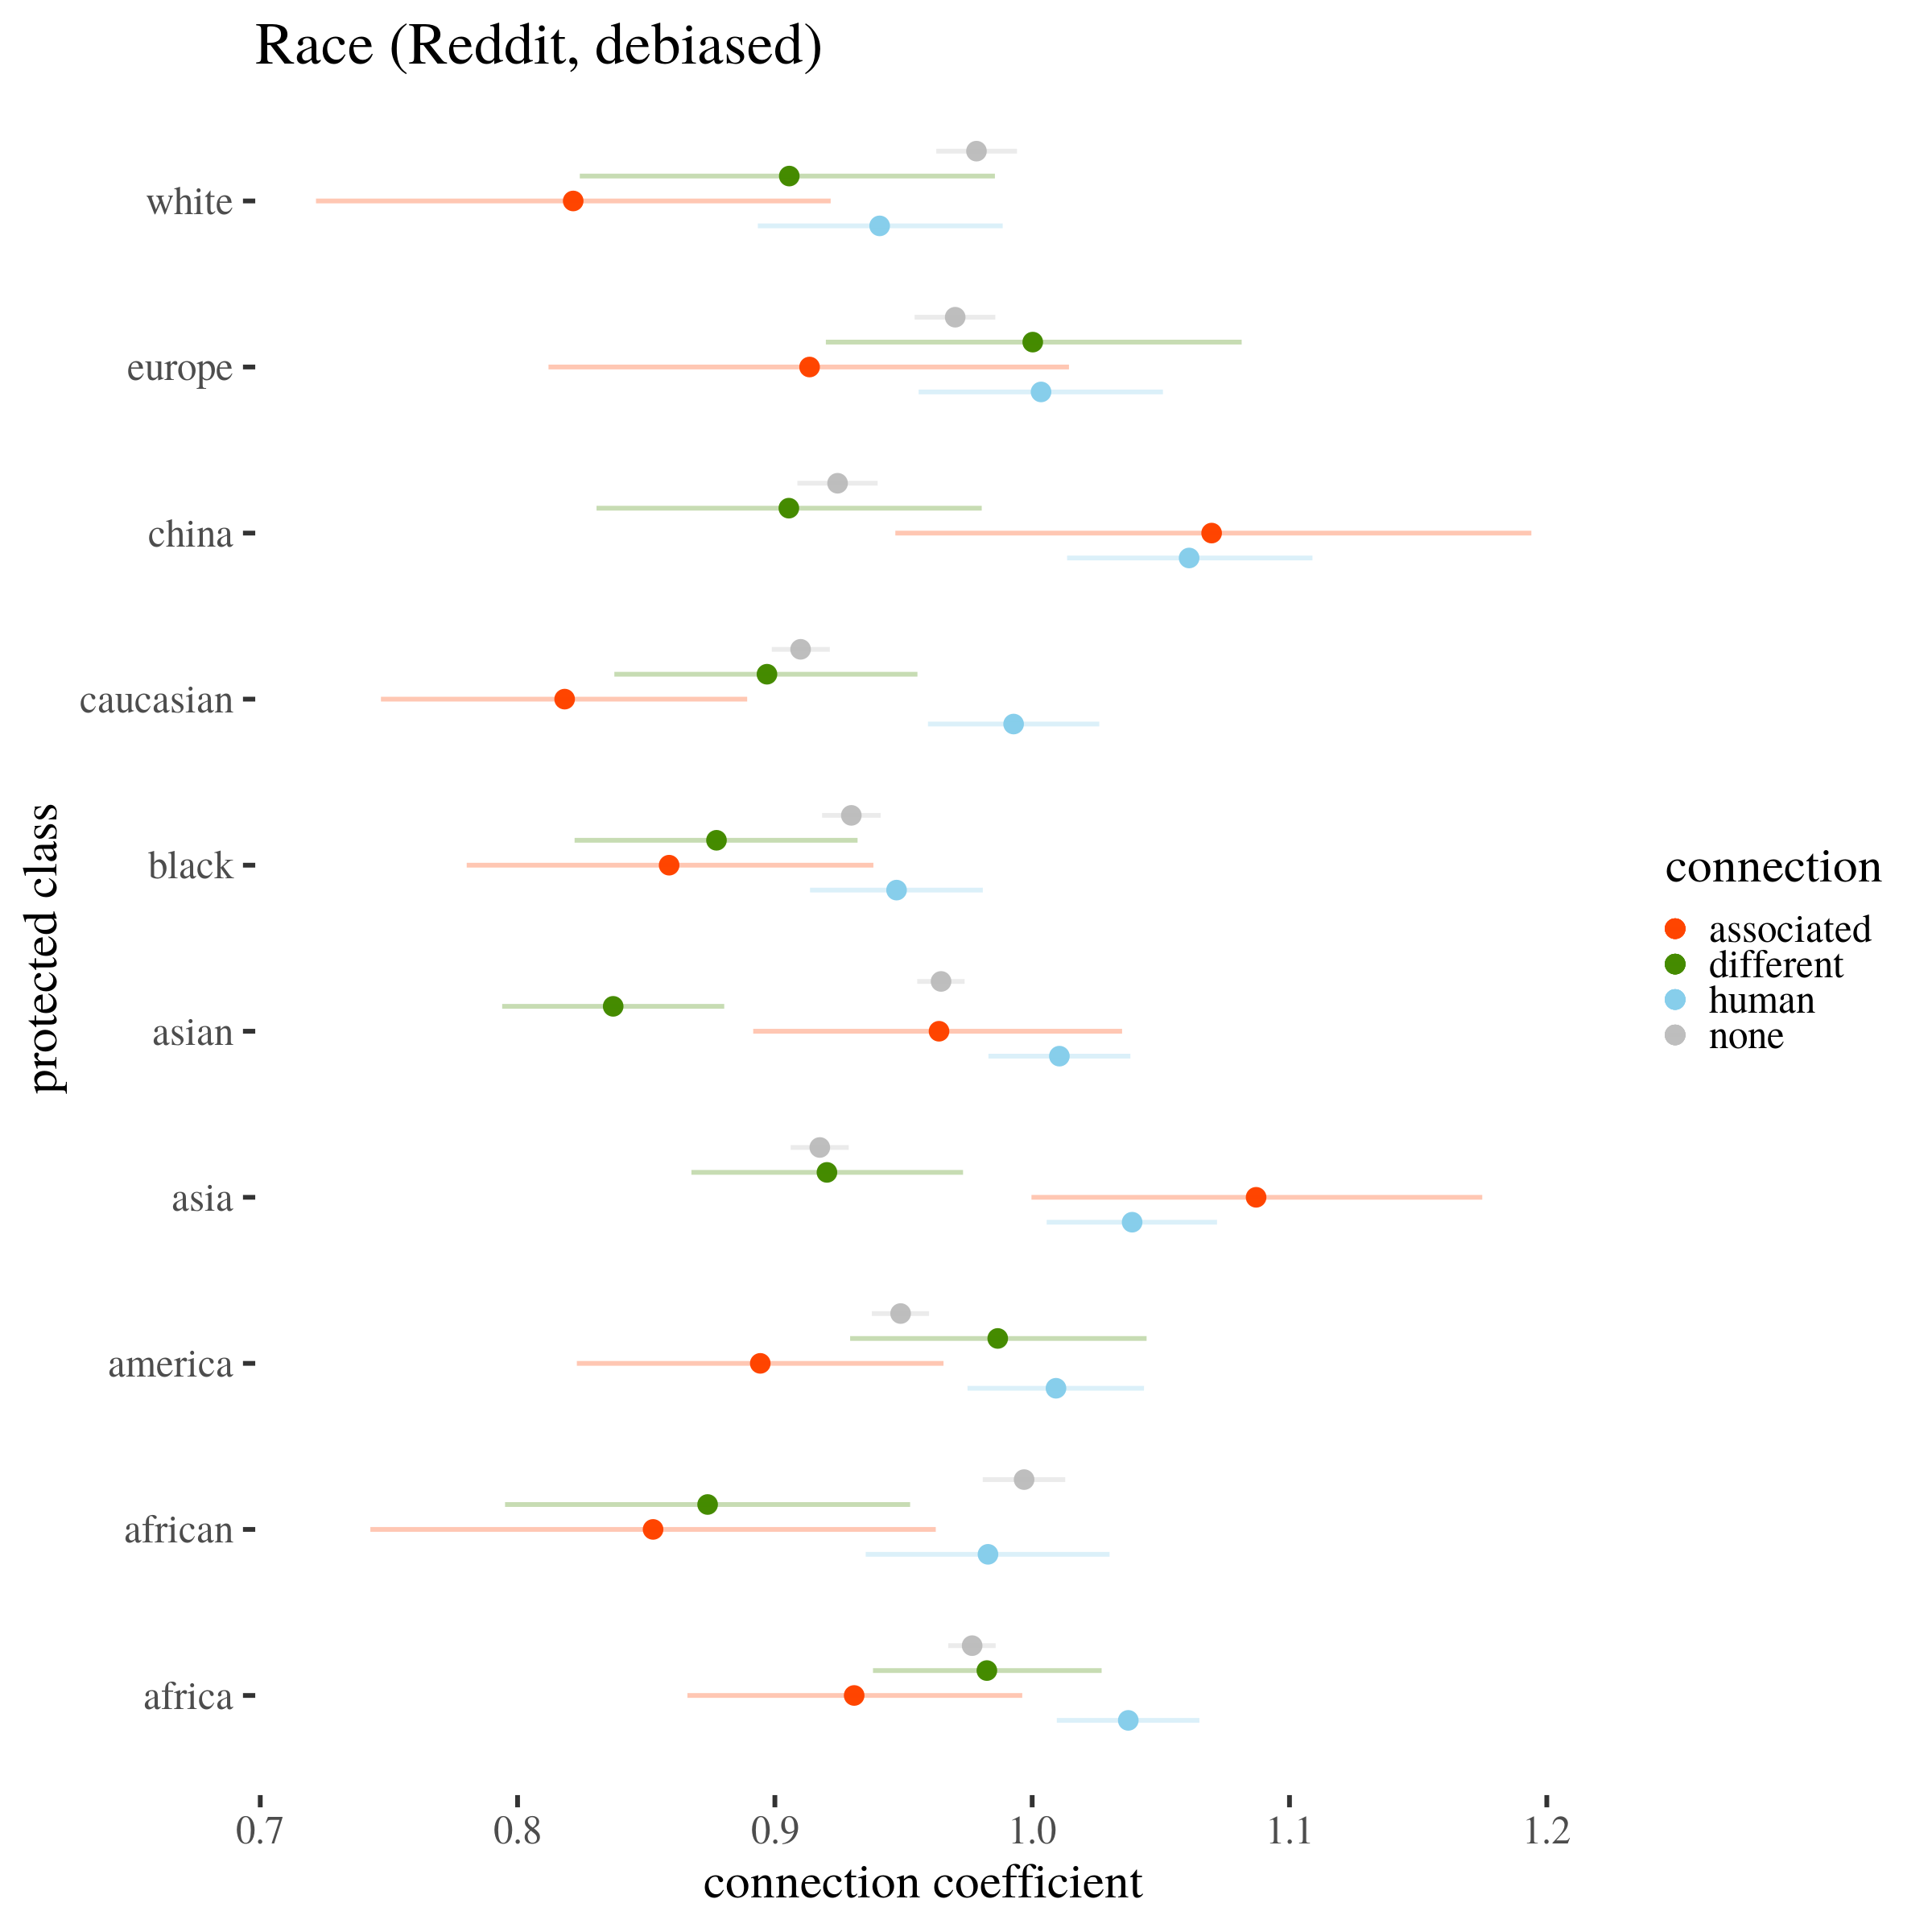
\includegraphics[width=14cm]{../images/visDebRaceReddit.png}

\chapter{Discussion}\label{discussion}

\hypertarget{refs}{}
\hypertarget{ref-Bolukbasi2016Man}{}
Bolukbasi, T., Chang, K., Zou, J. Y., Saligrama, V., \& Kalai, A.
(2016). Man is to computer programmer as woman is to homemaker?
Debiasing word embeddings. \emph{CoRR}, \emph{abs/1607.06520}. Retrieved
from \url{http://arxiv.org/abs/1607.06520}

\hypertarget{ref-Caliskan2017Semantics}{}
Islam, A. C., Bryson, J. J., \& Narayanan, A. (2016). Semantics derived
automatically from language corpora necessarily contain human biases.
\emph{CoRR}, \emph{abs/1608.07187}. Retrieved from
\url{http://arxiv.org/abs/1608.07187}

\hypertarget{ref-manzini2019black}{}
Manzini, T., Lim, Y. C., Tsvetkov, Y., \& Black, A. W. (2019). Black is
to criminal as caucasian is to police: Detecting and removing multiclass
bias in word embeddings.

\hypertarget{ref-Mehrabi2019Survey}{}
Mehrabi, N., Morstatter, F., Saxena, N., Lerman, K., \& Galstyan, A.
(2019). A survey on bias and fairness in machine learning. \emph{CoRR},
\emph{abs/1908.09635}. Retrieved from
\url{http://arxiv.org/abs/1908.09635}

\hypertarget{ref-Nissim2019Fair}{}
Nissim, M., Noord, R. van, \& Goot, R. van der. (2019). Fair is better
than sensational: Man is to doctor as woman is to doctor. \emph{CoRR},
\emph{abs/1905.09866}. Retrieved from
\url{http://arxiv.org/abs/1905.09866}

\end{document}
